\documentclass{template}
\usepackage{array}
\usepackage{graphicx}
\usepackage{float}
\usepackage{csquotes}
\usepackage[automake,acronym, toc=false]{glossaries-extra}

\hypersetup{
    pdftitle={Designing InterMind -- Entwicklung eines feministisch-digitalen Forschungsdesigns zur raumbezogenen Erfassung intersektional situierten (Un-)Wohlbefindens},
    pdfauthor={Lukas Batschelet},
    pdfsubject={Bachelorarbeit},
    pdfkeywords={Intersektionalität, Wohlbefinden, App, Erhebung, Geographie} 
}




\makeglossaries
%TC:ignore

\newacronym{esm}{ESM}{Experience Sampling Method}
\newacronym{ema}{EMA}{Ecological Momentary Assessment}
\newacronym{gema}{GEMA}{Geographically Explicit Ecological Momentary Assessment}
\newacronym{drm}{DRM}{Day Reconstruction Method}
\newacronym{panas}{PANAS}{The Positive \& Negative Affect Schedule}
\newacronym{maihda}{MAIHDA}{Multilevel Analysis of Individual Heterogeneity and Discriminatory Accuracy}
\newacronym[description={Intersectional MAIHDA -- siehe \gls[noindex]{maihda}}]{i-maihda}{I-MAIHDA}{Intersectional \gls[noindex]{maihda}}
\newacronym{cart}{CART}{Classification and Regression Trees}
\newacronym{json}{JSON}{JavaScript Object Notation}
\newacronym{dsg}{DSG}{Schweizer Datenschutzgesetz}
\newacronym{dsgvo}{DSGVO}{EuropäischeDatenschutz-Grundverordnung}
\newacronym{peqi}{PEQI}{Perceived Environmental Quality Indices}
\newacronym{news}{NEWS}{Neighborhood Environment Walkability Scale}
\newacronym{health}{HEALTH}{The Healthy Environments and Active Living for Translational Health Platform}
\newacronym{mvp}{MVP}{Minimum Viable Product}
\newacronym{cicd}{CI/CD}{Continuous Integration/Continuous Delivery}
\newacronym{esec}{ESec}{European Socio-economic Classification}
\newacronym{egp}{EGP}{Erikson–Goldthorpe–Portocarero-Klassenschema}
\newacronym{wemwbs}{WEMWBS}{Warwick-Edinburgh Mental Wellbeing Scale}
\newacronym{icc}{ICC}{Intra-Class Correlation}
\newacronym{pev}{PEV}{Proportional Explained Variance}





\newacronym{vgl}{vgl.}{vergleiche}
\newacronym{bspw}{bspw.}{beispielsweise}
\newacronym{gps}{GPS}{Global Positioning System}
\newacronym{zb}{z.\,B.}{zum Beispiel}
\newacronym{ua}{u.\,a.}{unter anderem}
\newacronym{etc}{etc.}{et cetera}
\newacronym{eng}{engl.}{englisch}
\newacronym{bzw}{bzw.}{beziehungsweise}


\newglossaryentry{race}{
    name={\textit{race}},
    description={Eine im englischsprachigen Raum etablierte, gesellschaftlich konstruierte Kategorie, die rassifizierende Zugehörigkeiten beschreibt. In dieser Arbeit kursiv gesetzt, um ihre soziokulturelle Bedeutung zu betonen und sie deutlich vom biologistischen Begriff \enquote{Rasse} abzugrenzen. Der Begriff verweist auf machtvolle Prozesse sozialer Differenzierung, Zugehörigkeit und Ausschluss, die historisch gewachsen sind und bis heute wirksam bleiben. Die Übertragung des Konzepts in europäische Kontexte ist umstritten: Aus Angst vor biologisierenden Implikationen und im Schatten nationaler Gewaltgeschichte (\gls{zb} Nationalsozialismus) wird \textit{race} oft durch vage Begriffe wie \enquote{Ethnizität} ersetzt oder gänzlich vermieden, was zur epistemischen Unsichtbarmachung rassifizierter Erfahrungen führen kann \parencite{bartelsPostcolonialFeminismIntersectionality2019}.},
    sort=race
}


\newglossaryentry{gender}{
    name={\textit{gender}},
    description={Eine gesellschaftlich konstruierte Kategorie, die auf soziale, kulturelle und politische Vorstellungen von Geschlecht verweist. \textit{gender} beschreibt normative Erwartungen an Geschlechtsidentität und Geschlechtsausdruck, die in spezifischen historischen und kulturellen Kontexten entstehen und sich verändern können. In dieser Arbeit kursiv gesetzt, um den Unterschied zum biologisierenden Begriff \enquote{sex} (\gls{eng}) \gls{bzw} \enquote{biologisches Geschlecht} hervorzuheben. Die Verwendung im Deutschen ist uneinheitlich: Während \textit{gender} in wissenschaftlichen Diskursen etabliert ist, wird es im Alltagsgebrauch häufig unscharf verwendet oder mit \enquote{Geschlecht} gleichgesetzt, was die soziale Konstruiertheit verwischt \parencite{butlerGenderTroubleFeminism1990}.},
    sort=gender
}

\newglossaryentry{schwarz}{
    name={Schwarz},
    description={Politische Selbstbezeichnung von Menschen, die im Kontext rassistischer Machtverhältnisse positioniert werden. Grossgeschrieben zur Abgrenzung von farblichen Zuschreibungen und um die Konstruktion von \enquote{Schwarzsein} als soziale Position zu betonen, nicht als biologische Eigenschaft. Die Schreibweise folgt postkolonialen und kritischen rassismustheoretischen Ansätzen, die die Erfahrung von Diskriminierung, Widerstand und Zugehörigkeit in den Vordergrund stellen \parencite{oguntoyeFarbeBekennenAfrodeutsche1986}.},
    sort=schwarz
}

\newglossaryentry{intersektionalitaet}{
    name={Intersektionalität},
    description={Analytisches Konzept zur Untersuchung sich überschneidender und wechselseitig verstärkender Machtverhältnisse wie Rassismus, Sexismus oder Klassismus. Entwickelt von Kimberlé Crenshaw zur Beschreibung der spezifischen Diskriminierungserfahrungen Schwarzer Frauen, die weder durch feministische noch durch antirassistische Theorien allein erfasst wurden. Der Ansatz betont, dass soziale Kategorien nicht additiv wirken, sondern in ihren Verflechtungen eigenständige Formen von Ungleichheit erzeugen. Heute wird er in einer Vielzahl disziplinärer und methodischer Kontexte angewandt, ist jedoch in seiner theoretischen Radikalität nicht unumstritten \parencite{crenshawMappingMarginsIntersectionality1991, collinsBlackFeministThought2002}.},
    sort=intersektionalitaet
}

\newglossaryentry{class}{
    name={\textit{class}},
    description={Eine gesellschaftlich konstruierte Kategorie, die ökonomische, kulturelle und symbolische Ungleichheiten beschreibt. \textit{class} verweist auf soziale Hierarchien, die sich aus Eigentum, Einkommen, Bildung, Beruf und anderen Ressourcen ergeben und historisch durch kapitalistische Strukturen geformt wurden. In dieser Arbeit kursiv gesetzt, um die soziale Konstruiertheit und die Differenz zum alltagssprachlichen Begriff \enquote{soziale Schicht} zu betonen. Die Übersetzung ins Deutsche ist umstritten, da Begriffe wie \enquote{Klasse} oder \enquote{Schicht} jeweils eigene theoretische Traditionen und politische Konnotationen mitbringen.},
    sort=class
}


\newglossaryentry{reactnative}{
  name={React Native},
  description={Ein Framework zur plattformübergreifenden Entwicklung mobiler Apps. Es erlaubt die Programmierung mit \gls[noindex]{javascript} oder \gls[noindex]{typescript}, wobei der Code nativ auf Android- und iOS-Geräten ausgeführt wird. \href{https://reactnative.dev/}{reactnative.dev}}
}

\newglossaryentry{expo}{
  name={Expo},
  description={Ein Toolchain und Dienst, der die Entwicklung mit \gls[noindex]{reactnative} vereinfacht. Expo stellt Werkzeuge zum Testen, Debuggen und Veröffentlichen von Apps bereit -- ohne dass native Programmierkenntnisse erforderlich sind. \href{https://expo.dev/}{expo.dev}}
}

\newglossaryentry{supabase}{
  name={Supabase},
  description={Ein Open-Source-Backend, das als Alternative zu Firebase dient. Es basiert auf einer \gls[noindex]{datenbank} (PostgreSQL) und bietet Funktionen wie Authentifizierung, Datei-Hosting und \gls[noindex]{rls}. \href{https://supabase.com/}{supabase.com}}
}

\newglossaryentry{javascript}{
  name={JavaScript},
  description={Eine weit verbreitete Programmiersprache für Webentwicklung, die auch in mobilen Frameworks wie \gls[noindex]{reactnative} verwendet wird. Sie ist dynamisch und flexibel, aber nicht typensicher.}
}

\newglossaryentry{typescript}{
  name={TypeScript},
  description={Eine von Microsoft entwickelte Programmiersprache, die auf \gls[noindex]{javascript} basiert, aber zusätzliche statische Typisierung bietet. Sie erhöht die Wartbarkeit und Fehlervermeidung in grösseren Softwareprojekten.}
}

\newglossaryentry{python}{
  name={Python},
  description={Eine interpretierte, einfach lesbare Programmiersprache, die häufig in Wissenschaft, Datenanalyse und Automatisierung eingesetzt wird. Sie wurde auch zur Auswertung der App-Daten verwendet.}
}

\newglossaryentry{uuid}{
  name={UUID},
  description={Abkürzung für Universally Unique Identifier. Eine \textit{UUID} ist eine zufällig generierte Zeichenkette, die zur eindeutigen Identifikation eines Geräts oder Datensatzes dient, ohne personenbezogene Daten zu erfassen.},
  first={Universally Unique Identifier (\glsentrytext{uuid})}
}

\newglossaryentry{opensource}{
  name={Open-Source},
  description={Bezeichnet Software, deren Quellcode öffentlich einsehbar, veränderbar und frei verwendbar ist. \gls[noindex]{supabase} und viele Komponenten von \gls[noindex]{reactnative} und \gls[noindex]{expo} sind Open-Source.}
}

\newglossaryentry{datenbank}{
  name={Datenbank},
  description={Ein digitales System zur strukturierten Speicherung, Abfrage und Verwaltung von Daten. In der App kommt eine relationale Datenbank zum Einsatz, die durch \gls[noindex]{supabase} bereitgestellt wird.}
}

\newglossaryentry{rls}{
  name={RLS},
  description={Ein feingranulares Zugriffsmodell in einer \gls[noindex]{datenbank}, das sicherstellt, dass Nutzer:innen nur jene Datenzeilen sehen oder ändern können, für die sie berechtigt sind. \gls[noindex]{supabase} unterstützt RLS standardmässig.},
  first={Row-Level Security (\glsentrytext{rls})}
}

\newglossaryentry{github}{
  name={GitHub},
  description={Eine webbasierte Plattform zur Versionsverwaltung und Zusammenarbeit an Softwareprojekten. Sie basiert auf \gls[noindex]{git} und wird häufig zur Entwicklung und Veröffentlichung von \gls[noindex]{opensource}-Software verwendet}
}

\newglossaryentry{git}{
  name={Git},
  description={Ein verteiltes Versionskontrollsystem zur Nachverfolgung von Änderungen im Quellcode. Git ermöglicht es, Entwicklungsschritte lokal oder kollaborativ zu verwalten und ist Grundlage vieler Plattformen wie \gls[noindex]{github}}
}

\newglossaryentry{frontend}{
  name={Frontend},
  description={Der Teil einer Software, der für Nutzer:innen sichtbar und direkt bedienbar ist -- etwa die Benutzeroberfläche einer App. Wird meist in Kombination mit dem \gls[noindex]{backend} verwendet.}
}

\newglossaryentry{backend}{
  name={Backend},
  description={Der Teil einer Software, der im Hintergrund läuft und Daten verarbeitet, speichert oder bereitstellt. In dieser Arbeit wird dafür \gls[noindex]{supabase} verwendet.}
}

\newglossaryentry{framework}{
  name={Framework},
  description={Ein vorgefertigtes Gerüst für die Softwareentwicklung, das häufig genutzte Funktionen bereitstellt. \gls[noindex]{reactnative} ist ein Beispiel für ein solches Framework.},
  plural={Frameworks}
}

\newglossaryentry{pushnotification}{
  name={Push-Benachrichtigung},
  description={Eine Mitteilung, die von einer App aktiv an das Gerät gesendet wird -- auch wenn die App im Hintergrund läuft. In dieser Studie werden so die Teilnehmenden zur Beantwortung der Fragen aufgefordert.},
  plural={Push-Benachrichtigungen}
}

\newglossaryentry{ui}{
  name={UI},
  description={Die Benutzeroberfläche einer App, die für Nutzer:innen sichtbar und direkt bedienbar ist. In dieser Arbeit wird die Benutzeroberfläche der App als \gls[noindex]{ui} bezeichnet.},
  first={User Interface (\glsentrytext{ui})}
}

\newglossaryentry{postgresql}{
  name={PostgreSQL},
  description={Eine relationale \gls[noindex]{datenbank}, die als \gls[noindex]{backend} für \gls[noindex]{supabase} verwendet wird.}
}

\newglossaryentry{urbanmind}{
  name={\textit{Urban Mind}},
  description={Eine mobile App zur Echtzeit-Erhebung subjektiven Wohlbefindens mittels \gls[noindex]{gema}. Die App erfasst affektive Zustände mehrfach täglich und verknüpft sie mit räumlichen Kontexten wie Naturerleben. \glslink[noindex]{intersektionalitaet}{Intersektionale} Perspektiven werden nicht systematisch berücksichtigt. Siehe \href{https://www.urbanmind.info/}{urbanmind.info}},
  first={Urban Mind},
  sort=urbanmind
}

\newglossaryentry{reliefmaps}{
  name={\textit{Relief Maps+}},
  description={Ein webbasiertes Tool zur retrospektiven und \glslink[noindex]{intersektionalitaet}{intersektionalen} Reflexion subjektiver Raumerfahrungen. Nutzer\genderstern innen verorten emotionale Bewertungen entlang von \glspl{identitaetsachse} auf einer Karte. Siehe \href{https://reliefmaps.upf.edu/}{reliefmaps.upf.edu}},
  first={Relief Maps+},
  sort=reliefmaps
}

\newglossaryentry{intermind}{
  name={\textit{InterMind}},
  description={Eine in dieser Arbeit entwickelte \gls[noindex]{opensource}-App zur \gls[noindex]{gema}-basierten Erhebung situativer Erfahrungen. Die Entwicklung wird in \cref{sec:entwicklung_app} beschrieben. Siehe \href{https://intermind.ch/}{intermind.ch}},
  sort=intermind
}

\newglossaryentry{identitaetsachse}{
  name={Identitätsachse},
  plural={Identitätsachsen},
  description={Begriff aus der \glslink[noindex]{intersektionalitaet}{intersektionalen} Theorie, der eine einzelne soziale Kategorie wie \gls[noindex]{gender}, \gls[noindex]{race}, \gls[noindex]{class}, sexuelle Orientierung, (Dis-)Ability oder Alter bezeichnet. Solche Achsen strukturieren gesellschaftliche Positionierungen und prägen Erfahrungen von Privilegierung oder Diskriminierung.}
}

\newglossaryentry{ios}{
  name={iOS},
  description={Eine mobile Betriebssystem-Plattform, die von Apple entwickelt wird. Sie wird hauptsächlich auf Geräten des iPhone- und iPad-Produktlinien verwendet.}
}

\newglossaryentry{android}{
  name={Android},
  description={Eine mobile Betriebssystem-Plattform, die von Google entwickelt wird. Sie wird hauptsächlich auf Geräten des Android-Produktlinien verwendet.}
}

\newglossaryentry{authentifizierung}{
  name={Authentifizierung},
  description={Vorgang zur Überprüfung der Identität eines Nutzers oder Geräts, typischerweise durch die Eingabe eines Passworts, Tokens oder durch kryptografische Verfahren. In der App erfolgt die Authentifizierung gerätebasiert mittels UUID, ohne Eingabe persönlicher Informationen}
}

\newglossaryentry{autorisierung}{
  name={Autorisierung},
  description={Festlegung von Zugriffsrechten auf bestimmte Ressourcen oder Daten nach erfolgreicher Authentifizierung. In diesem Projekt bedeutet dies, dass nur das eigene Gerät auf die jeweils verknüpften Datensätze zugreifen kann (Row-Level Security)}
}

\newglossaryentry{solid}{
  name={SOLID},
  description={Akronym für fünf grundlegende Prinzipien guter objektorientierter Softwarearchitektur: \textit{Single Responsibility, Open/Closed, Liskov Substitution, Interface Segregation, Dependency Inversion}. Die Prinzipien sollen verständliche, wartbare und erweiterbare Softwaresysteme ermöglichen \parencite{martinCleanArchitectureCraftsmans2018}}
}

\newglossaryentry{emulator}{
  name={Emulator},
  plural={Emulatoren},
  description={Softwareumgebung, die ein bestimmtes Betriebssystem oder Gerät auf einem anderen System simuliert, um Programme wie auf einem echten Gerät auszuführen. In der App-Entwicklung dienen Emulatoren insbesondere dem Testen von Anwendungen auf unterschiedlichen Bildschirmgrössen, Betriebssystemversionen und Gerätearchitekturen, ohne dass reale Geräte erforderlich sind}
}

\newglossaryentry{googleplayconsole}{
  name={Google Play Console},
  description={Plattform von \gls[noindex]{google} zur Verwaltung und Verteilung von \gls[noindex]{android}-Anwendungen. Sie ermöglicht die Veröffentlichung, das Testing und das Monitoring von Apps auf Geräten mit dem Betriebssystem \gls[noindex]{android}}
}

\newglossaryentry{testflight}{
  name={TestFlight},
  description={Offizielle Plattform von Apple zur Bereitstellung von \gls[noindex]{ios}-Apps für Betatests. Entwickler\genderstern innen können damit Vorabversionen ihrer Anwendungen an registrierte Testpersonen verteilen}
}

\newglossaryentry{java}{
  name={Java},
  description={Eine streng \glslink[noindex]{objektorientierung}{objektorientierte} Programmiersprache, die in vielen Bereichen der Softwareentwicklung eingesetzt wird.}
}

\newglossaryentry{objektorientierung}{
  name={Objektorientierung},
  description={Ein Programmierparadigma, das die Entwicklung von Software durch die Modellierung von Objekten und deren Interaktionen vereinfacht. In dieser Arbeit wird die \gls[noindex]{objektorientierung} verwendet, um die App strukturiert und wartbar zu halten.}
}

\newglossaryentry{githubissue}{
    name={GitHub-Issue},
    description={Ein integriertes Werkzeug zur Aufgaben- und Projektverwaltung auf der Plattform \gls[noindex]{github}. 
    GitHub-Issues dienen der strukturierten Erfassung, Diskussion und Nachverfolgung von Aufgaben, 
    Fehlern, neuen Funktionen oder allgemeinen Projektthemen. Sie können mit Labels, Meilensteinen 
    und Verantwortlichkeiten versehen werden, um Entwicklungsprozesse transparent und nachvollziehbar zu gestalten.},
    plural={GitHub-Issues}
}

\newglossaryentry{devops}{
  name={DevOps},
  description={Ein Konzept, das die Integration von Entwicklung und Operations zusammenführt, um schnellere und stabilere Softwareentwicklung zu ermöglichen. DevOps umfasst Tools und Prozesse, die die Automatisierung von Build, Test und Bereitstellung von Software unterstützen.}
}

\newglossaryentry{meta}{
    name={Meta},
    description={US-Technologiekonzern, \gls[noindex]{ua} Entwickler von Facebook, Instagram, WhatsApp und \gls[noindex]{reactnative}.}
}

\newglossaryentry{google}{
    name={Google},
    description={US-Technologiekonzern, \gls[noindex]{ua} Betreiber von Suchmaschine, Google Play Store, YouTube und Entwickler von \gls[noindex]{firebase}.}
}

\newglossaryentry{apple}{
    name={Apple},
    description={US-Technologiekonzern, Hersteller von iPhone und Betreiber des App Store.}
}

\newglossaryentry{firebase}{
    name={Firebase},
    description={Ein \gls[noindex]{backend}-as-a-Service von \gls[noindex]{google}, das Authentifizierung, Datenspeicherung und Schnittstellenbereitstellung integriert bereitstellt.}
}

\newglossaryentry{refactoring}{
  name={Refactoring},
  description={Der Prozess der Verbesserung der Struktur und Lesbarkeit von Code, ohne dass sich die Funktionalität ändert. Refactoring ist ein wichtiger Bestandteil der Softwareentwicklung, um Code-Qualität zu erhöhen und Wartbarkeit zu verbessern.}
}

\newglossaryentry{stratum}{
    name={Stratum},
    plural={Strata},
    description={Bezeichnung für eine Teilmenge einer Grundgesamtheit in der Statistik, gebildet nach gemeinsamen Merkmalen der darin enthaltenen Beobachtungen.}
}




%TC:endignore

% common abkürzungen beim ersten mal nicht ausführen
\glsunset{vgl}
\glsunset{bspw}
\glsunset{gps}
\glsunset{zb}
\glsunset{ua}
\glsunset{etc}
\glsunset{hiv}
\glsunset{gis}
\glsunset{kap}
\glsunset{s}

\glsadd{vgl}
\glsadd{bspw}
\glsadd{gps}
\glsadd{zb}
\glsadd{ua}
\glsadd{etc}
\glsadd{hiv}
\glsadd{gis}
\glsadd{kap}
\glsadd{s}



\AddBibFile{BA_Lukas_Batschelet.bib}


\begin{document}
\pagenumbering{Roman}


\includepdf[pages=1]{Arbeit/Titelblatt/Titelblatt_digital.pdf}

\clearpage
\pagenumbering{roman}

Diese Bachelorarbeit entwickelt und dokumentiert ein kritisch-digitales, quantitatives Forschungsdesign zur raumbezogenen Erfassung situierten (Un\nobreakdash-)Wohlbefindens aus intersektionaler Perspektive. Theoretisch knüpft die Arbeit an emotionale Geographien und Intersektionalität an und versteht Wohlbefinden als kontextgebundene, situative Erfahrung, die durch räumliche und soziale Lagen mitgeprägt wird. Methodisch verbindet sie den \glsxtrshort{ema}/\glsxtrshort{gema}-Ansatz mit einer offenen, nachvollziehbaren Forschungsinfrastruktur: Mit der eigens entwickelten App InterMind werden wiederholte, geolokalisierte Befragungen im Alltag erhoben; Code und Workflows sind quelloffen und auf Transparenz, Nachnutzbarkeit und Datenschutz (Privacy by Design) ausgelegt. Eine explorative Pilotierung dient der Prüfung von Machbarkeit, Erhebungslogistik, Datenqualität und Nutzererfahrung sowie der Frage, ob die Datenstruktur für intersektionale Mehrebenenmodelle (\glsxtrshort[noindex]{i-maihda}) geeignet ist. Die Pilotstudie verfolgt ausdrücklich keinen inhaltlichen Wirksamkeitsnachweis; sie validiert Prozesse und macht methodische Grenzen sichtbar. Der Beitrag der Arbeit liegt in (1) der Bereitstellung eines offenen Werkzeugs für kontextsensitive Wiederholungsmessungen, (2) der sorgfältigen Dokumentation eines reproduzierbaren Analysepfads und (3) einer reflektierten methodischen Einordnung, die Anschlussstellen für grössere, heterogenere Stichproben und weiterführende Mixed-Methods-Studien aufzeigt.

\vfill
\noindent
Diese Arbeit ist lizenziert unter einer 
\href{https://creativecommons.org/licenses/by-sa/4.0/}
{CC BY-SA 4.0 Lizenz}. \ccbysa

\cleardoublepage



\begingroup
  \fontsize{10.4pt}{0.9em}\selectfont
  \setlength{\parskip}{0pt}
  \setlength{\itemsep}{0pt plus 0.02pt}
  \tableofcontents\null
\endgroup

\begingroup
\makeatletter
\renewcommand*{\glossarypreamble}{%
  \addcontentsline{toc}{chapter}{Abkürzungsverzeichnis}%
}
\makeatother


% Glossar ohne erzwungenen Seitenumbruch
\begingroup
  \fontsize{10.4pt}{0.9em}\selectfont
  \setstretch{1.1}
  \printglossary[
    type=\acronymtype,
    nonumberlist,
    title=Abkürzungsverzeichnis,
    nogroupskip,
  ]
\endgroup



\begingroup
  \let\clearpage\relax
  \let\cleardoublepage\relax
  \listoffigures
  \listoftables
\endgroup


\clearpage
\pagenumbering{arabic}
% LTeX: language=de-CH
\chapter{Einleitung} \label{sec:einleitung}

In einer datenjournalistischen Auswertung zeigt sich, dass Hitzeinseln in Schweizer Städten ungleich verteilt sind und häufiger ärmere Quartiere betreffen \parencite{albisserUngleichheitStaedtenHitzeinseln2023}. Temperatur ist jedoch nur einer von vielen Faktoren, die alltägliches (Un-)Wohlbefinden prägen; dieses entsteht in komplexen, situativen Konstellationen aus räumlichen Anordnungen, Regeln, Routinen und sozialen Positionierungen. So reduziert die Analyse von Hitzeinseln Ungleichheit letztlich auf die Kopplung einer Exposition (Temperatur) mit einem Einzelmerkmal (sozioökonomischer Status), während viele Differenzen tiefer in soziale und räumliche Ordnungen verwoben sind und sich als flüchtige, kontextabhängige Erfahrungen im Raum zeigen. Vor diesem Hintergrund entwickle und erprobe ich in dieser Arbeit ein Forschungsdesign, das solche situativen Erfahrungen des (Un-)Wohlbefindens kontextualisiert, wiederholt und ortsnah erfassbar macht und für intersektional sensible Analysen anschlussfähig ist.

Ich beziehe mich dafür auf das Feld der \emph{emotional} und \emph{affective geographies}, die alltägliche Gefühle und ihre räumlichen Dimensionen untersuchen \parencite{hoSocialGeographyIII2024}. Dieses Forschungsfeld zeigt, dass Erfahrungen von (Un-)Wohlbefinden nicht rein individuell sind, sondern relational entstehen: Sie knüpfen an materielle Umgebungen, soziale Machtstrukturen und an die Positionierung von Körpern im Raum. Damit bieten sich mir ein theoretisches Fundament, um (Un-)Wohlbefinden als situierte Erfahrung zu verstehen, die zugleich flüchtig und strukturiert, persönlich erlebt und gesellschaftlich geformt ist.

Zugleich arbeite ich mit einem intersektionalen Verständnis von Ungleichheiten. Erfahrungen lassen sich nicht entlang einzelner sozialen Kategorien -- etwa \gls[noindex]{gender}, \emph{Alter} oder \gls[noindex]{class}\footnotemark -- erklären, sondern nur in ihrer Verschränkung. Ich gehe davon aus, dass Diskriminierungen und Privilegien nicht additiv nebeneinanderstehen, sondern sich in ihrem Zusammenspiel gegenseitig verstärken, überlagern oder abschwächen.

\footnotetext{Soziale Kategorien wie \gls[noindex]{race}, \gls[noindex]{gender}, \gls[noindex]{class}, \emph{Alter} oder \emph{Behinderung} werden in dieser Arbeit kursiv gesetzt, um ihre Bedeutung als sozial konstruierte, wandelbare und gesellschaftlich wirkungsmächtige Kategorien hervorzuheben. Die Begriffe \gls[noindex]{race}, \gls[noindex]{gender} und \gls[noindex]{class} werden zudem in englischer Sprache verwendet, da ihre deutschen Übersetzungen in der wissenschaftlichen Debatte umstritten sind. Ausführlichere Erläuterungen finden sich im \nameref{sec:glossary}.}

Gerade im Zusammenspiel dieser beiden Perspektiven ergibt sich eine forschungspraktische Herausforderung: Zwar gibt es zahlreiche qualitativ ausgerichtete Studien, die emotionale Erfahrungen und intersektionale Positionierungen in alltäglichen Situationen beschreiben, jedoch fehlen bislang methodische Ansätze, mit denen sich solche Dynamiken systematisch und quantitativ erfassen lassen. Nur wenige Versuche existieren,  (Un-)Wohlbefinden in seiner räumlich-situativen und intersektionalen Dimension zugleich systematisch und quantitativ zu erfassen. Mit dieser Arbeit möchte ich deshalb einen Beitrag dazu leisten, intersektionale Ungleichheiten auch in quantitativen Forschungsdesigns sichtbar zu machen -- ein Bereich, der in der Geographie bislang kaum entwickelt ist.

\vspace{1em}

Aus dieser Leerstelle ergibt sich die zentrale Forschungsfrage dieser Arbeit:
\begin{quote}
\emph{Wie lässt sich der Einfluss räumlicher Umgebungen auf das situierte (Un-)Wohlbefinden intersektional positionierter Personen erfassen und analysieren?}
\end{quote}

Zur Bearbeitung dieser Leitfrage formuliere ich drei spezifische Teilfragen, die deren Beantwortung aus methodischer, infrastruktureller und empirischer Perspektive vorbereiten:

\begin{enumerate}
    \item Wie muss ein Forschungsdesign gestaltet sein, um situiertes (Un-)Wohlbefinden intersektional positionierter Personen gemeinsam mit relevanten Kontextmerkmalen wiederholt zu erfassen?
    \item Welche Anforderungen ergeben sich aus einer kritisch-digitalen Perspektive an eine Infrastruktur, die solche Erhebungen ermöglicht, und wie lassen sich diese praktisch umsetzen?
    \item Welche Möglichkeiten und Grenzen bieten die erhobenen Daten im Hinblick auf eine intersektionale Mehrebenenmodellierung?
\end{enumerate}

Die Beantwortung dieser Fragen erfordert einen Ansatz, der wiederholte Befragungen im Alltag mit räumlichem Bezug ermöglicht. Als Methodische Basis verwende ich dafür die \gls{ema}-Methode, die darauf abzielt, Erfahrungen möglichst unmittelbar im jeweiligen Kontext zu erfassen. Erweiterungen im Sinne der \gls{gema}-Methode beziehen zusätzlich situative Umgebungsbedingungen ein und ermöglichen so beispielsweise, über Standortdaten auch Einflüsse wie Temperatur und Bebaunungsstruktur zu erfassen. In der Geographie werden beide Methoden bislang jedoch nur vereinzelt angewendet, obwohl sie ein hohes Potenzial bieten, den Einfluss räumlicher Kontexte systematisch zu untersuchen.

Für die Durchführung von \gls{ema}- und \gls{gema}-Studien existieren verschiedene digitale Infrastrukturen. Ich zeige in dieser Arbeit auf, dass diese entweder proprietär sind oder ihre Datenverarbeitung nur teilweise nachvollziehbar ist. Für die Erhebung sensibler Daten stellt dies eine zentrale Einschränkung dar: Wenn unklar bleibt, wie Daten gespeichert, verarbeitet oder weitergegeben werden, widerspricht dies den Prinzipien von Transparenz, Datensparsamkeit und Nachvollziehbarkeit. Aus einer kritisch-digitalen Perspektive ist deshalb eine offene Infrastruktur erforderlich, die den gesamten Datenfluss überprüfbar macht und die Kontrolle über die erhobenen Daten sowohl bei den Teilnehmenden als auch bei den Forschenden belässt.

Vor diesem Hintergrund entwickle ich in dieser Arbeit mit der App \gls[noindex]{intermind}\footnotemark eine quelloffene Erhebungsplattform für \gls{ema}- und \gls{gema}-Studien. \gls[noindex]{intermind} ermöglicht wiederholte Befragungen im Alltag, erfasst Standortdaten und setzt dabei auf eine transparente und sichere Datenverarbeitung. Die offene Auslegung schafft die Grundlage für eine langfristig nutzbare, überprüfbare Infrastruktur zur Erhebung kontextualisierter Alltagsdaten.

\footnotetext{Ich habe mich dazu entschieden, nach der im Rahmen dieser Arbeit durchgeführten Datenerhebung, die App wieder aus den App Stores zu entfernen. In \cref{sec:diskussion} begründe ich diese Entscheidung ausführlicher. Der Quellcode der App ist vollständig auf \gls[noindex]{github} (\href{https://github.com/lbatschelet/InterMind}{github.com/lbatschelet/InterMind}) unter einer \gls{lic:agpl}-Lizenz veröffentlicht.}

In einer explorativen Pilotstudie erprobe ich das entwickelte Forschungsdesign aus Infrastruktur, Erhebungsdesign und Auswertungspfad. Dabei prüfe ich, ob die erhobenen Daten die nötige Differenzierung und Qualität für eine intersektionale Mehrebenenanalyse aufweisen und wo die Grenzen des Ansatzes liegen. Ziel ist der methodische Machbarkeitsnachweis, nicht die Generalisierung inhaltlicher Effekte.

Der Aufbau der Arbeit folgt einer klaren Abfolge von theoretischer Rahmung, methodischer Herleitung und empirischer Umsetzung. In \Cref{sec:theoretischer_rahmen} führe ich zentrale Konzepte ein: \gls{intersektionalitaet} als Analyseperspektive, situiertes (Un-)Wohlbefinden als Gegenstand sowie kritisch-digitale Ansätze als Leitlinie für die Gestaltung der Forschungsinfrastruktur. Darauf aufbauend verorte ich die Arbeit in \Cref{sec:methodik} im Feld wiederholter Alltagsbefragungen und diskutiere, wie sich diese mit intersektionalen Auswertungsansätzen verbinden lassen. 

Im Anschluss wende ich mich der praktischen Umsetzung zu: In \Cref{sec:entwicklung_app} beschreibe ich die Entwicklung der offenen App \gls[noindex]{intermind}, bevor ich in \Cref{sec:fragebogenentwicklung} die Konstruktion des Fragebogens darstelle. Die Durchführung und Auswertung der Pilotstudie präsentiere ich in \Cref{sec:pilotstudie}. Den Abschluss bildet \Cref{sec:diskussion}, in der ich zentrale Befunde reflektiere, methodische Implikationen diskutiere und Perspektiven für künftige Forschung skizziere.

Mit dieser Arbeit ziele ich darauf, methodische Potenziale einer intersektionalen, kontextnahen Erhebung von situiertem (Un-)Wohlbefinden sichtbar zu machen und eine Grundlage für künftige Anwendungen zu schaffen.




\clearpage

% LTeX: language=de-CH

\chapter{Verflechtungen verstehen -- Begriffe und Konzepte} \label{sec:theoretischer_rahmen}

In diesem Kapitel führe ich in die zentralen Begriffe und Konzepte ein, die das Erkenntnisinteresse leiten und das methodische Vorgehen rahmen. Ausgangspunkt ist eine intersektionale Perspektive, mit der ich gesellschaftliche Unterschiede nicht isoliert, sondern in ihrer wechselseitigen Verflechtung analysiere. Anschliessend entfalte ich das Konzept des situierten (Un-)Wohlbefindens als kontextabhängige, räumlich gebundene Erfahrung. Ergänzend nehme ich eine digitale Perspektive ein, die fragt, wie Daten, digitale Infrastrukturen und technologische Gestaltungsprozesse gesellschaftliche Machtverhältnisse widerspiegeln und (re)produzieren. Zusammen stelle ich diese Perspektiven als Grundlage für ein Forschungsdesign vor, das soziale Positionierung, räumliche Kontexte, situative Erfahrungen und digitale Infrastrukturen in Beziehung setzt.

\section{Verwebte Unterschiede -- Intersektionalität als Analyseinstrument}

Gesellschaftliche Wirklichkeiten sind durchzogen von komplexen Ungleichheiten. Menschen erfahren soziale Benachteiligung selten entlang nur einer einzigen Achse -- vielmehr wirken verschiedene Differenzlinien wie \gls{race}, \gls{gender} oder \gls{class} häufig gleichzeitig und verstärken sich wechselseitig. So kann die Erfahrung einer migrantischen Frau auf dem Arbeitsmarkt nicht einfach in \enquote{sexistische} und \enquote{rassistische} Diskriminierung zerlegt werden. Ihre Benachteiligung ergibt sich vielmehr aus der spezifischen Verschränkung dieser Positionierungen, die durch keine einzelne Kategorie vollständig erfasst wird. In dieser Arbeit beziehe ich mich deshalb auf einen intersektionalen Ansatz, um diese Verflechtungen zu erfassen und einen Rahmen zu produzieren, der Ungleichheitsverhältnisse nicht isoliert betrachtet, sondern ihre Überschneidungen und Wechselwirkungen berücksichtigt.

Geprägt wird der Begriff der \gls{intersektionalitaet} von \textcite{crenshawMappingMarginsIntersectionality1991}, die auf die spezifischen Diskriminierungserfahrungen \emph{\glslink{schwarz}{Schwarzer}}\footnotemark Frauen aufmerksam macht. In ihrer Analyse von Antidiskriminierungsklagen im US-amerikanischen Arbeitsrecht zeigt sie, dass \emph{\glslink{schwarz}{Schwarze}} Frauen häufig keinen Rechtsschutz erhielten. Gerichte verhandelten Diskriminierung entweder als \emph{\gls{gender} discrimination} oder als \emph{\gls{race} discrimination}, jedoch nicht in der Verschränkung beider Kategorien. Wurde eine Klage als \emph{\gls{gender} discrimination} geprüft, erfolgte der Vergleich mit weissen Frauen; blieben diese unbetroffen, galt die Klage als unbegründet. Wurde sie als \emph{\gls{race} discrimination} geprüft, erfolgte der Vergleich mit \emph{\glslink{schwarz}{Schwarzen}} Männern; auch hier verschwanden die spezifischen Benachteiligungen \emph{\glslink{schwarz}{Schwarzer}} Frauen. Ihre Erfahrungen fielen damit durch die Raster der bestehenden Rechtskategorien und blieben juristisch unsichtbar. Crenshaw argumentiert, dass feministische und antirassistische Theorien in ähnlicher Weise unzureichend sind, um Mehrfachdiskriminierung zu erfassen, und entwickelt \gls{intersektionalitaet} als analytisches Instrument zur Beschreibung solcher überlagerten Ungleichheitsverhältnisse \parencite[\gls{vgl}][]{hancockWhenMultiplicationDoesnt2007}.

\footnotetext{Ich schreibe den Begriff \enquote{\gls{schwarz}} mit grossem Anfangsbuchstaben und verwende ihn als politische Selbstbezeichnung von Menschen, die im Kontext rassistischer Machtverhältnisse positioniert werden. Der Begriff bezeichnet keine biologistische Eigenschaft, sondern eine soziale Positionierung; die Grossschreibung dient der Abgrenzung von äusserlichen Zuschreibungen \parencite{oguntoyeFarbeBekennenAfrodeutsche1986}. }

Ausgangspunkt dieser theoretischen Perspektive ist der Black Feminist Thought, welcher unter anderen in den Arbeiten von \textcite{hooksAintWomanBlack1981}, \textcite{lordeSisterOutsiderEssays1984}, Kimberle~\textcite{crenshawMappingMarginsIntersectionality1991} und \textcite{collinsBlackFeministThought2002} ihren Ausdruck findet. Black Feminist Thought formuliert eine scharfe Kritik an traditionellen feministischen Ansätzen, denen vorgeworfen wird, primär die Erfahrungen weisser, privilegierter Frauen ins Zentrum zu stellen und somit die Lebensrealitäten \emph{\glslink{schwarz}{Schwarzer}} Frauen zu marginalisieren. \textcite{crenshawMappingMarginsIntersectionality1991} entwickelt das Konzept der \gls{intersektionalitaet} explizit als Reaktion auf die Unfähigkeit bestehender theoretischer Ansätze, die spezifischen Diskriminierungserfahrungen \emph{\glslink{schwarz}{Schwarzer}} Frauen adäquat zu erfassen. Dabei verdeutlicht sie, dass Diskriminierung nicht als Summe einzelner, isolierter Erfahrungen verstanden werden kann, sondern als eigenständige Form sozialer Benachteiligung, die sich an der Überschneidung sozialer Kategorien wie \gls{race} und \gls{gender} manifestiert.

\gls{intersektionalitaet} entwickelte sich nicht allein im akademischen Kontext, sondern ist eng mit den politischen Kämpfen sozialer Bewegungen der 1970er- und 1980er-Jahre verbunden, insbesondere im Umfeld feministischer, antirassistischer und antikapitalistischer Strömungen \parencite{collinsBlackFeministThought2002}. Diese Bewegungen machten sichtbar, dass unterschiedliche Formen sozialer Ungleichheit nicht isoliert nebeneinander existieren, sondern in ihrer Verschränkung erfahrbar werden. Damit legten sie die Grundlage für eine Perspektive, die gesellschaftliche Differenzen nicht als additive Kategorien, sondern als strukturell verknüpfte Machtverhältnisse versteht.

Zentral für die theoretische Fundierung des intersektionalen Ansatzes ist die Einsicht, dass soziale Positionierungen historisch gewachsen und gesellschaftlich konstruiert sind. Kategorien wie \gls{gender}, \gls{race} oder \gls{class} können daher nicht ohne Bezug auf die Macht- und Herrschaftsordnungen verstanden werden, in denen sie entstanden sind. Sie wirken nicht nur beschreibend, sondern ordnen Zugänge zu Ressourcen, Rechten und gesellschaftlicher Teilhabe.

Autorinnen wie Audre Lorde und bell hooks verdeutlichten, dass diese strukturellen Machtverhältnisse nicht abstrakt bleiben, sondern konkrete Auswirkungen auf individuelle Lebensrealitäten haben. Lorde betonte die Bedeutung von Differenz als Quelle von Wissen und Widerstand, während hooks die alltägliche Reproduktion patriarchaler und rassistischer Herrschaftsverhältnisse analysierte \parencite{collinsBlackFeministThought2002, hancockWhenMultiplicationDoesnt2007}. Damit trugen sie entscheidend dazu bei, Intersektionalität als kritisches Instrument zu etablieren, das sowohl strukturelle Dimensionen von Ungleichheit als auch subjektive Erfahrungen in den Blick nimmt.

Von der ursprünglich starken Fokussierung auf \textit{race} und \textit{gender} wird das Konzept in den folgenden Jahrzehnten zunehmend erweitert und schliesst heute oft eine Vielzahl sozialer Positionierungen und Identitäten ein, darunter etwa \emph{Sexualität}, \emph{Alter}, \emph{Behinderung}, \emph{Nationalität} oder \emph{Religion} \parencite{bauerIntersectionalityQuantitativeResearch2021, bowlegInvitedReflectionQuantifying2016}. Diese Erweiterung verdeutlicht die breite theoretische und empirische Anwendbarkeit von \gls{intersektionalitaet} als Analyseinstrument zur kritischen Untersuchung gesellschaftlicher Ungleichheiten und Diskriminierungserfahrungen. \gls{intersektionalitaet} hat sich somit nicht nur als theoretisches Konzept, sondern auch als methodische Grundlage etabliert, welche insbesondere in feministisch und sozialwissenschaftlich orientierten Diskursen verwendet wird, um die komplexen Wechselwirkungen gesellschaftlicher Machtverhältnisse zu analysieren.

\vspace{2em}

Die Anwendung intersektionaler Perspektiven auf räumliche Fragestellungen stellt eine zentrale Weiterentwicklung des ursprünglichen Konzepts der \gls{intersektionalitaet} dar. Seit den 2000er-Jahren etablierte sich eine eigenständige geographische Perspektive, die räumliche Kontextualität und situative Dimensionen sozialer Ungleichheiten explizit in den Mittelpunkt rückt \parencite{valentineTheorizingResearchingIntersectionality2007,rodo-de-zarateIntersectionalityFeministGeographies2018}.

Zentral für diesen Perspektivwechsel ist das Verständnis von Raum als gesellschaftlich produzierter Grösse. \textcite{lefebvreProductionLespace1974} betont, dass Raum kein neutrales Behältnis ist, in dem soziale Prozesse einfach stattfinden, sondern ein Produkt sozialer Praktiken, Aushandlungen und Machtbeziehungen. Raum entsteht durch Planung, Nutzung und alltägliche Routinen -- etwa durch Wohnungs- und Stadtbaupolitik, durch Verkehrs- und Infrastrukturen oder durch symbolische Markierungen wie Namen, Grenzen und Symbole. Machtverhältnisse schreiben sich in diese Strukturen ein und wirken dadurch stabilisierend: Wer Zugang zu bestimmten Räumen hat, wer ausgeschlossen bleibt oder wie Räume bewertet werden, reproduziert gesellschaftliche Hierarchien.

\textcite{foucaultEspacesAutres2004} erweitert diese Perspektive mit dem Konzept der Heterotopien. Damit bezeichnet er Räume, die gesellschaftliche Normen zugleich widerspiegeln und infrage stellen. Solche Räume sind ambivalent: Sie können dominante Ordnungen stabilisieren, indem sie Abweichungen räumlich „einschliessen“ (wie etwa Gefängnisse, Kliniken oder Kasernen), oder sie können alternative Formen des Zusammenlebens sichtbar machen (wie etwa Gärten, Festivals oder subkulturelle Treffpunkte). Heterotopien machen deutlich, dass Räume nicht nur materielle Anordnungen sind, sondern gesellschaftliche Ordnungen verkörpern und potenziell auch verschieben können.

Auf dieser theoretischen Grundlage argumentiert \textcite{valentineTheorizingResearchingIntersectionality2007}, dass soziale Kategorien nicht unabhängig vom Raum wirken. Ihre Bedeutung entfaltet sich erst im Zusammenspiel mit konkreten räumlichen Kontexten. Valentine zeigt dies am Beispiel muslimischer Frauen in britischen Städten. Ihre Erfahrungen im öffentlichen Raum sind nicht überall gleich, sondern variieren je nach Ort und sozialer Situation: In bestimmten Strassen oder Nachbarschaften sind sie aufgrund sichtbarer religiöser Zugehörigkeit -- etwa durch das Tragen eines Kopftuchs -- rassistischen und sexistischen Anfeindungen ausgesetzt. Dieselben Frauen erleben in anderen Kontexten, zum Beispiel in Moscheen, Community-Zentren oder stärker divers geprägten Quartieren, Sicherheit, Zugehörigkeit und Anerkennung. Entscheidend ist damit nicht allein die soziale Positionierung, sondern deren situative Übersetzung in räumliche Erfahrungen. Der Raum fungiert nicht als neutraler Hintergrund, sondern als aktiver Vermittler, der Zugehörigkeit ermöglichen oder ausschliessen kann. Ungleichheiten sind somit nicht nur verteilt im Raum, sondern werden durch räumliche Anordnungen hervorgebracht und für unterschiedliche Gruppen in spezifischer Weise erfahrbar gemacht.

\textcite{mccallComplexityIntersectionality2005} unterscheidet drei methodische Zugänge zu \gls{intersektionalitaet}. Der \emph{interkategoriale} Ansatz vergleicht festgelegte soziale Kategorien miteinander, um deren Überschneidungen sichtbar zu machen -- etwa indem Lohnunterschiede zwischen \emph{\glslink{schwarz}{Schwarzen}} Frauen, weissen Frauen, \emph{\glslink{schwarz}{Schwarzen}} Männern und weissen Männern analysiert werden. Der \emph{intrakategoriale} Ansatz richtet den Blick auf Unterschiede innerhalb einer einzelnen Kategorie, insbesondere dort, wo diese intern heterogen ist. So kann etwa untersucht werden, wie sich die Erfahrungen von Frauen unterscheiden, je nachdem ob sie gleichzeitig rassistische oder klassistische Diskriminierung erfahren. Der \emph{antikategoriale} Ansatz schliesslich stellt die Stabilität und analytische Nützlichkeit solcher Kategorien grundsätzlich infrage und fragt, ob festgelegte Identitätsachsen nicht selbst Teil des Problems sind.

Diese Systematisierung hat auch in geographischen Arbeiten Bedeutung erlangt, da sie methodisch begründet, wie sich verschiedene Dimensionen sozialer Differenz in räumlichen Analysen miteinander verknüpfen lassen. McCall betont zudem, dass \gls{gender} nicht isoliert betrachtet werden kann, sondern als interdependente Kategorie zu verstehen ist, deren Wirkung nur im Zusammenspiel mit anderen Differenzachsen entsteht \parencite{mccallSpatialRoutesGender1998}. Diese Wechselwirkungen sind wiederum stets in spezifische räumliche und historische Kontexte eingebettet, die ihre Ausprägung und Bedeutung prägen.

Empirische Arbeiten in der Geographie operationalisieren diese theoretischen Ansätze auf unterschiedliche Weise. Ein frühes Beispiel liefert \textcite{mccallSpatialRoutesGender1998}, die mit multilevel-statistischen Analysen regionale Strukturen und geschlechtsspezifische Lohnunterschiede verknüpft. Auch wenn ihre Arbeit der expliziten intersektionalen Wende in der Geographie noch vorausgeht, verdeutlicht sie, wie sich interkategoriale Zugänge nutzen lassen, um räumliche Muster sozialer Disparitäten sichtbar zu machen. \textcite{fensterRightGenderedCity2005} entwickelt diese Perspektive weiter, indem sie narrative und ethnographische Methoden einsetzt, um alltägliche Erfahrungen von Frauen in städtischen Kontexten zu untersuchen. Sie zeigt, dass das Konzept des „Right to the City“ patriarchale Machtverhältnisse unzureichend berücksichtigt und dass Zugehörigkeit und Teilhabe durch geschlechtsspezifische Ausschlüsse strukturiert sind. Mit einem dezidiert intersektionalen Anspruch führt \textcite{rodo-de-zarateDevelopingGeographiesIntersectionality2014} schliesslich ein Instrument ein, das soziale Positionierungen, emotionale Dimensionen und Orte systematisch miteinander verbindet. Die \emph{Relief Maps} ermöglichen es, subjektive Erfahrungen räumlicher Ungleichheit nicht nur zu erfassen, sondern auch visuell darzustellen und vergleichbar zu machen.

\vspace{2em}

Obwohl intersektionale Forschung historisch in qualitativen und aktivistischen Traditionen verankert ist, gewinnen quantitative Verfahren zunehmend an Relevanz, insbesondere in sozialpolitischen und raumplanerischen Kontexten \parencite{bauerIntersectionalityQuantitativeResearch2021}. Diese Verfahren bieten die Möglichkeit, strukturelle Muster intersektionaler Benachteiligung über grössere Stichproben sichtbar und empirisch überprüfbar zu machen.

Neuere methodische Entwicklungen wie \gls{i-maihda} \parencite[\gls{ua}][]{evansMultilevelApproachModeling2018,bellExtendingIntersectionalMultilevel2023} versuchen, dieser Herausforderung zu begegnen, indem sie intersektionale Positionierungen nicht als feste Gruppenmerkmale behandeln, sondern als dynamische, verschachtelte Konstellationen modellieren. Solche Ansätze zeigen, dass auch quantitative Forschung produktiv an intersektionale Theorien anschliessen kann. Gerade in der Geographie eröffnet dies die Möglichkeit, intersektionale Ungleichheiten nicht nur statistisch nachzuzeichnen, sondern auch in ihrer räumlichen Dimension sichtbar zu machen.

Jedoch ist die Übertragung intersektionaler Theorien in quantitative Methoden mit erheblichen Herausforderungen verbunden. Zentral ist die Kritik, dass traditionelle statistische Verfahren soziale Kategorien oft eindimensional oder additiv behandeln, was der komplexen theoretischen Vorstellung intersektionaler Verschachtelungen nicht gerecht wird \parencite{hancockWhenMultiplicationDoesnt2007, bowlegInvitedReflectionQuantifying2016}. Insbesondere birgt die numerische Operationalisierung sozialer Identitäten die Gefahr, die Fluidität und Kontextabhängigkeit dieser Kategorien zu ignorieren und damit ungewollt jene komplexen Wechselwirkungen zu nivellieren, die intersektionale Ansätze ursprünglich sichtbar machen wollen \parencite{scottIntersectionalityQuantitativeMethods2017}.

Um diesen Herausforderungen zu begegnen, bedarf es einer reflexiven und kontextsensiblen Operationalisierung intersektionaler Kategorien. Dies beinhaltet, soziale Gruppen nicht als statische Entitäten zu behandeln, sondern ihre relationalen und kontextuellen Eigenschaften explizit zu berücksichtigen \parencite{rodo-de-zarateDevelopingGeographiesIntersectionality2014, websterCenteringSocialtechnicalRelations2021}.


\section{Gefühlte Orte -- Situiertes (Un-)Wohlbefinden als räumliche Erfahrung}

(Un-)Wohlbefinden ist flüchtig und kontextabhängig. In diesem Abschnitt versuche ich zu entwickeln, wie Situationen entstehen, in denen Orte, Praktiken, Atmosphären und Positionierungen (Un-)Wohlbefinden ermöglichen oder begrenzen.

In den Sozial- und Gesundheitswissenschaften kursieren unterschiedliche Konzepte von Wohlbefinden, die jeweils eigene theoretische Setzungen und politische Implikationen mittragen. Der aus der Psychologie stammende Begriff \enquote{Subjektives Wohlbefinden} wird häufig über standardisierte Skalen erfasst und als individuelle Eigenschaft begriffen. Kritische sozialwissenschaftliche und feministische Perspektiven -- einschliesslich geographischer Arbeiten -- weisen darauf hin, dass dieses Verständnis hochgradig individualisiert ist und zu einer neoliberalen Regierungstechnik werden kann: Es verlagert Verantwortung auf Einzelne und blendet strukturelle Ungleichheiten, zeitliche und räumliche Skalen sowie Relationen aus \parencite{atkinsonToxicEffectsSubjective2021}. Sichtbar wird dies in politischen Wohlbefindens-Indizes wie dem \emph{World Happiness Report} oder nationalen Befragungen, die Lebenszufriedenheit über Einzelfragen messen und politische Steuerung an individuelle Bewertungen koppeln. Auch Corporate-Wellbeing-Programme oder Public-Health-Strategien, die auf Resilienztrainings und Lifestyle-Optimierung setzen, illustrieren diese Tendenz: Sie fördern Anpassung an bestehende Strukturen, anstatt ungleiche Lebensbedingungen oder diskriminierende Machtverhältnisse zu problematisieren \parencite[\gls{vgl}]{atkinsonToxicEffectsSubjective2021}. Diese Kritik motiviert eine stärker relationale, räumlich-kontextualisierte und machtsensible Fassung von Wohlbefinden.

Das Konzept des \enquote{affektiven Wohlbefindens} ist zentral in den \emph{affective geographies} verankert \parencite{hoSocialGeographyIII2024}. Wohlbefinden wird hier nicht als rein innerer Zustand verstanden, sondern als Ergebnis von räumlichen Anordnungen, sozialen Praktiken und Atmosphären. \textcite{ahmedAffectiveEconomies2004} analysiert dies am Beispiel politischer Diskurse in den USA, etwa auf Webseiten der \emph{Aryan Nations}. Sie zeigt, wie Emotionen wie Hass oder Angst nicht einfach \enquote{individuell} entstehen, sondern als \enquote{affective economies} zwischen Körpern, Symbolen und Orten zirkulieren. Indem etwa Migration oder Diversität mit Bedrohung verknüpft wird, \enquote{haften} Emotionen an bestimmten Körpern und Orten -- und schaffen dadurch Zugehörigkeiten für \enquote{weisse} einerseits und Abgrenzungen gegenüber \enquote{Anderen} andererseits.

Zugleich problematisiert \textcite{hemmingsInvokingAffectCultural2005} den sogenannten \emph{affective turn} in den Kultur- und Sozialwissenschaften. Sie kritisiert insbesondere die Tendenz, Affekte als vorsprachliche, universelle Intensitäten zu deuten. Eine solche Lesart, so Hemmings, droht Unterschiede und Machtverhältnisse auszublenden, weil sie affektive Erfahrungen von historischen und sozialen Kontexten ablöst. Für diese Arbeit ist deshalb entscheidend, affektive Dimensionen mitzudenken, ohne sie zu naturalisieren: Affekte werden hier als historisch und sozial situierte Relationen verstanden, die in konkreten räumlichen Konstellationen (Un-)Wohlbefinden hervorbringen.

\textcite{smithWhichBeingWellbeing2018} entwickeln als Gegenentwurf zu individualisierten Konzepten das Verständnis eines \enquote{intra-aktiven Wohlbefindens}. Sie greifen auf Karen Barads (\citeyear{baradMeetingUniverseHalfway2007}) Theorie des Agentiellen Realismus zurück, die davon ausgeht, dass Entitäten nicht unabhängig voneinander existieren und erst nachträglich in Relation treten, sondern dass sie durch materielle und diskursive \emph{Intra-Aktionen} überhaupt erst entstehen. Diese Perspektive verschiebt den Blick: Wohlbefinden ist nicht länger eine Eigenschaft isolierter Subjekte, sondern ein Effekt von Verflechtungen zwischen Menschen, Atmosphären, Infrastrukturen, Technologien und Dingen. Damit rückt eine \emph{more-than-human}-Lesart ins Zentrum, die die Mitwirkung materieller Umwelten und nicht-menschlicher Akteure ernst nimmt. 

Für die geographische Forschung eröffnet dieses Konzept neue Anschlussmöglichkeiten, etwa indem auch die Gestaltung von Stadträumen, die Materialität von Wohnumgebungen oder die Rolle digitaler Infrastrukturen als konstitutiv für Erfahrungen von (Un-)Wohlbefinden verstanden werden können. Zugleich bleibt dieser Zugang sprachlich schwer zugänglich und in der Wellbeing-Forschung bislang wenig etabliert, was seine Übertragung in empirische Studien erschwert.

Vor diesem Hintergrund verwende ich in dieser Arbeit den Begriff \emph{situiertes (Un-)Wohlbefinden}. Er knüpft an \textcite{leeUnderstandingDisruptedParticipation2021} an, die den Begriff in der Analyse von Sport- und Freizeitpraktiken eingeführt haben, sowie an feministische Epistemologien situierten Wissens \parencite{harawaySituatedKnowledgesScience1988}. Mit dieser Begriffswahl möchte ich Wohlbefinden nicht als innere, universelle Eigenschaft oder rein individuelles Affektgeschehen fassen, sondern als relationales, machtsensibles Erleben, das in spezifischen räumlichen und sozialen Konstellationen hervorgebracht wird. 

Die Schreibweise \enquote{(Un-)} macht sichtbar, dass negative Erfahrungen wie Ausschluss, Angst oder Unsicherheit analytisch gleichwertig zu positiven Momenten von Zugehörigkeit oder Sicherheit sind und nicht lediglich als Abweichungen von einem \enquote{normalen} Zustand von Wohlbefinden verstanden werden dürfen. 

Der Begriff \emph{situiert} verweist in dreifacher Hinsicht auf die theoretische Rahmung dieser Arbeit: Erstens betont er die Verkörperung und Kontextgebundenheit von Erfahrung, die nicht unabhängig von Orten, Atmosphären oder Praktiken gedacht werden kann. Zweitens rückt er die Rolle von Machtverhältnissen und intersektionaler Positionierungen in den Vordergrund, durch die Wohlbefinden ermöglicht oder eingeschränkt wird. Drittens markiert er eine erkenntnistheoretische Haltung, wie sie \textcite{harawaySituatedKnowledgesScience1988} formuliert: Wissen -- und in diesem Fall Erfahrung -- ist stets perspektivisch, partiell und situiert, niemals neutral oder allumfassend. 

Mit dem Konzept des \emph{sitiuierten (Un-)Wohlbefindens} ziele ich darauf, eine begriffliche Brücke zu schlagen: zwischen affektiven und atmosphärischen Dynamiken, den politischen Dimensionen von Macht und Zugehörigkeit sowie einer epistemologischen Reflexion über die Bedingungen, unter denen Wohlbefinden überhaupt erfahrbar und analysierbar wird.

\vspace{1em}

Aus dieser begrifflichen Herleitung folgt für meine Arbeit: Wenn (Un-)Wohlbefinden als \emph{situiert} verstanden wird, muss gezeigt werden, \emph{wie} Situationen entstehen. Ich greife dafür das Konzept kollektiver Stimmungen und Atmosphären auf, das eine analytische Ebene eröffnet, über die das Zusammenspiel von Orten, Praktiken und Machtverhältnissen erfahrbar wird und konkrete Verkörperungen von (Un-)Wohlbefinden sichtbar werden.

\textcite{andersonAffectiveAtmospheres2009} versteht unter \emph{affective atmospheres} kollektive, nicht vollständig repräsentierbare Stimmungen, die im Zusammenspiel räumlicher Faktoren (\gls{zb} Sichtachsen, Beleuchtung, Dichte, Lärm, Überwachung) und sozialer Ordnungen (\gls{zb} Zugangsregime, informelle Normen) entstehen. Atmosphären sind dabei nicht einfach die Summe dieser Elemente, sondern überschreiten sie, indem sie als schwer fassbare Qualitäten wirken, die zugleich materiell gebunden und flüchtig, bestimmt und unbestimmt sind. Sie prägen situativ (Un-)Wohlbefinden und erklären, warum derselbe Ort für unterschiedliche Gruppen gegensätzlich wirken kann. Ein stark kontrollierter Eingangsbereich oder ein nächtlicher Platz mag für privilegierte Gruppen belebt und angenehm erscheinen, während er für marginalisierte Gruppen als belastend oder bedrohlich erfahrbar ist. Diese Differenzen sind nicht allein individualpsychologisch, sondern in intersektionalen Machtverhältnissen verankert.

Solche Machtverhältnisse lassen sich über Zugehörigkeitsordnungen analytisch fassen. \textcite{antonsichSearchingBelongingAnalytical2010} versteht Zugehörigkeit nicht als stabilen Status, sondern als relationalen, umkämpften Prozess und unterscheidet zwischen \emph{place-belongingness} (Gefühle des Dazugehörens) und \emph{politics of belonging} (Regeln und Grenzziehungen, die Zugehörigkeit herstellen und begrenzen). \textcite{painGlobalizedFearEmotional2009} zeigt in diesem Sinn, wie Sicherheit und Unsicherheit affektiv-geopolitisch produziert werden -- durch Überwachung, Kontrolle, mediale Diskurse oder lokale Praktiken. Solche Prozesse lassen sich als \emph{bordering} fassen \parencite[\gls{vgl}][]{yuval-davisBelongingPoliticsBelonging2006}: Sie materialisieren sich in Blicken, räumlichen Markierungen oder scheinbar neutralen Routinen des Zugangs und wirken damit unmittelbar in Atmosphären hinein. Zugehörigkeit und Ausschluss werden so nicht abstrakt, sondern leiblich-situativ erfahrbar und strukturieren (Un-)Wohlbefinden.

Besonders prägnant illustriert dies \textcite{ahmedPhenomenologyWhiteness2007} mit einer phänomenologischen Analyse von \emph{Whiteness} im alltäglichen Raum. Sie argumentiert, dass Räume in mehrheitlich weissen Gesellschaften implizit auf weisse Körper ausgerichtet sind: Bewegungen wie das Betreten öffentlicher Gebäude verlaufen für sie \enquote{unmarkiert} und selbstverständlich. Nicht-weisse Körper dagegen stossen in denselben Situationen auf Widerstände -- etwa durch häufigere Polizeikontrollen, Blicke oder subtile Praktiken der Exklusion. Während weisse Subjekte sich im öffentlichen Raum mit einem Gefühl von Selbstverständlichkeit bewegen können, erfahren nicht-weisse Subjekte dieselben Orte als potenziell feindlich oder begrenzend. \emph{Whiteness} erscheint damit nicht nur als soziale Position, sondern als räumliche Orientierung, die alltägliche Handlungsräume strukturiert und die affektive Erfahrung von Vertrautheit oder Bedrohung ungleich verteilt.

\textcite{bissellPassengerMobilitiesAffective2010} zeigt am Beispiel von Zugfahrten, wie Atmosphären nicht nur als diffuse Stimmungen, sondern als leiblich-situative Kräfte wirksam werden. In überfüllten oder besonders lauten Waggons verdichten sich etwa Gereiztheit und Anspannung, sodass Fahrgäste bewusst bestimmte Abteile meiden, länger stehen oder Umwege in Kauf nehmen. Solche Atmosphären entstehen aus der Verschränkung körperlicher Dispositionen (Müdigkeit, Schmerz, sensorische Empfindlichkeit) mit materiellen Arrangements (Enge, Sitzordnung, Überwachung) und sozialen Erwartungen und prägen dadurch mikro-leibliche Praktiken des Alltags. Damit macht Bissell Atmosphären körperlich und situativ fassbar: Wohlbefinden im Raum lässt sich nicht nur über strukturelle Zugehörigkeitsordnungen begreifen, sondern auch über verkörperte Rhythmen und Affekte, die in Bewegung, Stillstand und alltäglichen Routinen entstehen.

Für die vorliegende Arbeit ziehe ich daraus drei analytische Konsequenzen: (1) (Un-)Wohlbefinden ist als \emph{kontextabhängiger Effekt} konkreter räumlich-sozialer Konstellationen zu untersuchen, nicht als innere Eigenschaft von Individuen; (2) Unterschiede im Erleben sind \emph{macht- und positionssensibel} zu lesen, das heisst intersektional verortet und durch Zugehörigkeitsordnungen strukturiert; (3) empirische Zugänge müssen \emph{verkörperte, situative Dynamiken} erfassen, ohne die situative Einbettung zu verlieren.

\vspace{1em}

Situiertes (Un-)Wohlbefinden wird in der Geographie auf unterschiedlichen Massstabsebenen (scales) untersucht. Ein Fokus auf körpernahe, individuelle Erlebnisse erlaubt es, feinste situative Veränderungen des Wohlbefindens zu erfassen -- etwa wie sich Stress oder Entspannung im direkten Kontakt mit spezifischen Orten oder Personen zeigt. Auf einer meso-räumlichen Ebene geraten kollektive Atmosphären in Quartieren, Stadtteilen oder anderen lokalisierten Gemeinschaftsräumen in den Blick, zum Beispiel Nachbarschaften, in denen Sicherheit, Lärm oder soziale Dichte das gemeinsame Erleben prägen. Makro-räumliche Analysen beziehen hingegen nationale oder transnationale Strukturen ein -- etwa migrationspolitische Rahmenbedingungen oder globale Ungleichheitsordnungen --, die emotionale Erfahrungen rahmen und begrenzen \parencite{howittScaleRelationMusical1998,marstonHumanGeographyScale2005}. Dieses skalierende Verständnis macht deutlich, dass situiertes (Un-)Wohlbefinden weder rein individuell noch vollständig lokal erklärbar ist, sondern immer in ein Geflecht aus Mikroerfahrungen, kollektiven Dynamiken und übergeordneten gesellschaftlich-räumlichen Strukturen eingebettet ist.

Die Geographie nutzt dieses skalierende Verständnis, um Fragen räumlicher Gerechtigkeit und sozialer Teilhabe zu untersuchen. Indem Mikroerfahrungen des Alltags mit kollektiven Dynamiken und übergeordneten gesellschaftlich-räumlichen Strukturen in Beziehung gesetzt werden, lassen sich ungleiche Verteilungen von Möglichkeiten, Sicherheit oder Zugang sichtbar machen. Damit wird situiertes (Un-)Wohlbefinden zu einem analytischen Zugang, der alltägliche emotionale Erfahrungen mit den Macht- und Ungleichheitsverhältnissen verknüpft, in die sie eingebettet sind.

\section{Digitale Werkzeuge -- Data Feminism, Open Source und digitale Souveränität}
\label{sec:datafeminism}

Digitale Technologien strukturieren zunehmend gesellschaftliche Realitäten -- sie beeinflussen, was sichtbar wird, wie Wissen entsteht und wer daran teilhat. Wer Software verwendet oder entwickelt, Daten sammelt oder Infrastrukturen kontrolliert, gestaltet diese Prozesse aktiv mit. Digitale Technologien sind daher nie neutral, sondern Ausdruck bestehender Machtverhältnisse. Eine kritische Auseinandersetzung mit digitalen Technologien und Infrastrukturen muss deshalb deren soziale und politische Dimension systematisch in den Blick nehmen.

Einen geeigneten theoretischen Rahmen hierfür bietet das Konzept des \textit{Data Feminism} von \textcite{dignazioDataFeminism2020}. Ausgangspunkt ist die Einsicht, dass Daten nie neutral sind, sondern stets Ausdruck gesellschaftlicher Machtverhältnisse. Sie entstehen nicht in einem Vakuum, sondern in konkreten sozialen, politischen und ökonomischen Kontexten, die prägen, was überhaupt als \enquote{Daten} gilt, wie sie erhoben werden und welche Fragen damit gestellt werden können. Data Feminism fordert deshalb, diese Bedingungen systematisch offenzulegen. Nur so wird sichtbar, dass Daten nicht einfach objektive Abbilder einer Realität darstellen, sondern mitbestimmen, was sichtbar wird und was unsichtbar bleibt. In diesem Sinne haben Daten eine konstitutive Funktion: Sie machen bestimmte Erfahrungen zähl- und vergleichbar, während andere Perspektiven ausgeblendet oder gar unsichtbar gemacht werden.

Damit knüpft Data Feminism an intersektionale Analysen an, die verdeutlichen, dass Ungleichheiten nicht entlang einer einzigen sozialen Kategorie erklärt werden können, sondern sich über mehrere Achsen wie Geschlecht, Klasse, Ethnizität oder Alter verschränken. Genau diese Verschränkung macht sichtbar, dass auch in Datenpraktiken Ausschlüsse und Hierarchien reproduziert werden: Wer gezählt wird, wer eine eigene Kategorie erhält, wessen Erfahrungen in Zahlen übersetzt werden und wessen nicht -- all das ist Ergebnis sozialer Aushandlungen und Machtbeziehungen. Die zentrale Erkenntnis von Data Feminism liegt darin, dass Daten zweischneidig sind: Sie können zur Stabilisierung bestehender Ungleichheiten beitragen, etwa indem sie dominante Kategorien unhinterfragt fortschreiben. Gleichzeitig können sie aber auch als Werkzeuge genutzt werden, um Machtasymmetrien offenzulegen, marginalisierte Perspektiven sichtbar zu machen und gerechtere Wissensordnungen zu schaffen.

Für die eigene Arbeit bedeutet das, dass Daten nicht einfach als technische Ressource betrachtet werden dürfen, sondern als soziale Praxis, die kritisch reflektiert werden muss. Data Feminism sensibilisiert dafür, dass auch methodische Entscheidungen -- welche Variablen erhoben werden, welche Kategorisierungen vorgenommen werden, wie Ergebnisse dargestellt werden -- nie rein technisch sind, sondern normative Annahmen transportieren. Diese Perspektive eröffnet die Möglichkeit, Datenerhebung nicht nur kritisch zu hinterfragen, sondern auch aktiv so zu gestalten, dass vielfältige Erfahrungen sichtbar werden und bestehende Ausschlüsse nicht weiter verstärkt werden. Damit liefert das Konzept eine wichtige Grundlage für eine Forschung, die soziale Gerechtigkeit nicht nur thematisiert, sondern auch methodisch einlöst.

\vspace{1em}

Digitale Infrastrukturen sind nicht nur technische Systeme, sondern Ausdruck und Austragungsorte gesellschaftlicher Machtverhältnisse. Im Anschluss an feministische Geographien lassen sie sich als Räume verstehen, in denen Fragen von Sichtbarkeit, Teilhabe und Gerechtigkeit immer wieder neu verhandelt werden \parencite{elwoodFeministDigitalGeographies2018}. Datenpraktiken und digitale Technologien erhalten damit eine politische Dimension: Sie strukturieren, wer Zugang hat, welche Perspektiven sichtbar werden und wie Wissen in Infrastrukturen eingeschrieben ist.

So zeigen \textcite{dignazioGeographiesMissingData2024} anhand einer Untersuchung von 33 zivilgesellschaftlichen Monitoring-Initiativen gegen Feminizide in 15 Ländern, wie digitale Praktiken zur Gegen-Datenproduktion eingesetzt werden können. Diese Initiativen reagieren auf systematische Leerstellen staatlicher und institutioneller Statistiken, in denen Gewalt an Frauen und queeren Personen unsichtbar bleibt. Indem sie eigene Datenbanken aufbauen, einzelne Fälle dokumentieren und in transnationale Netzwerke einspeisen, schaffen sie Räume der Erinnerung und Solidarität. Diese Praktiken machen deutlich, dass digitale Infrastrukturen nicht nur Gewalt sichtbar machen, sondern auch als Mittel widerständiger Raumpolitik fungieren können: Sie eröffnen Orte, an denen alternative Wissensordnungen etabliert werden und gesellschaftliche Machtverhältnisse herausgefordert werden.

Diese Beispiele zeigen, dass digitale Infrastrukturen nicht nur technische Artefakte, sondern politische Räume sind, in denen Fragen nach Kontrolle, Zugang und Gestaltungsmacht neu verhandelt werden. In wissenschaftlichen und politischen Debatten wird dieser Aushandlungsprozess zunehmend unter dem Begriff der digitalen Souveränität gefasst.

Während digitale Souveränität in politischen Diskursen häufig auf die Ebene nationalstaatlicher Strategien oder technischer Fähigkeiten verengt wird -- etwa im Kontext staatlicher Programme für Rechenzentren oder regulierter Datenflüsse --, verschiebt eine geographische Perspektive den Fokus auf ihre räumlichen Dimensionen. Politisch-geographische Arbeiten betonen, dass digitale Souveränität nicht einfach gegeben ist, sondern in spezifischen räumlichen Ordnungen hervorgebracht und verhandelt wird \parencite{glaszeContestedSpatialitiesDigital2023}.

So zeigen \textcite{glaszeContestedSpatialitiesDigital2023}, dass digitale Souveränität in unterschiedlichen Kontexten -- etwa in der EU und in Russland -- zwar auf ähnliche Leitbilder verweist, in der praktischen Umsetzung jedoch stark divergiert. Klassische Vorstellungen von Souveränität, Territorialität und staatlicher Kontrolle konfigurieren sich im digitalen Raum neu: Cloud-Computing, Plattformökonomien oder transnationale Datenströme erzeugen räumliche Spannungen, die weder allein durch nationale Gesetze noch durch technische Standards aufgelöst werden können. Damit wird digitale Transformation nicht als neutraler Modernisierungsprozess, sondern als politisch und räumlich situierte Auseinandersetzung sichtbar.

Auch \textcite{zhangBordersBorderingSovereignty2023} heben hervor, dass digitale Souveränität immer mit Prozessen der Grenzziehung verknüpft ist. Sie zeigen, dass diese digitalen Grenzen keineswegs nur an staatlichen Territorien verlaufen, sondern auf unterschiedlichen Massstabsebenen entstehen: von geopolitischen Regulierungen bis hin zu geschlossenen WhatsApp-Gruppen oder plattforminternen Zugangsbarrieren. Solche digitalen Grenzen strukturieren, wer Zugang zu Informationen und Infrastrukturen erhält, wer ausgeschlossen bleibt und wie digitale Räume angeeignet werden können.

Vor diesem Hintergrund lässt sich digitale Souveränität nicht als ortloses Prinzip begreifen, sondern als Ergebnis konkreter räumlicher Praktiken, Infrastrukturen und Machtverhältnisse. Eine kritische Perspektive versteht darunter zugleich die kollektive Fähigkeit, digitale Infrastrukturen nicht nur zu nutzen, sondern sie auch kritisch zu reflektieren, partizipativ zu gestalten und als Gemeingüter zugänglich zu machen \parencite{baackDataficationEmpowermentHow2015}. 

\vspace{1em}

\gls{opensource}-Praktiken können in diesem Zusammenhang als konkrete Werkzeuge einer relational verstandenen digitalen Souveränität gelesen werden. \textcite{gurumurthyDataBodiesNew2022} argumentieren aus einer feministischen Perspektive, dass Souveränität über Daten nicht allein durch individuelle Kontrolle oder \enquote{data ownership} gewährleistet werden kann. Sie zeigen am Beispiel von Menstruations-Apps, dass solche Ansätze oft unzureichend sind, um strukturelle Machtasymmetrien im Datenregime zu adressieren. Stattdessen fordern sie, Daten als \emph{social knowledge commons} zu verstehen und kollektive Praktiken der Kontrolle und Gestaltung in den Vordergrund zu stellen. In dieser Logik erscheint \gls{opensource} nicht nur als technisches Modell, sondern als relationales Prinzip, das auf Kooperation, geteilte Verantwortung und eine feministische Ethik der Datenpraktiken verweist.

Einen verwandten Zugang eröffnet \textcite{baackDataficationEmpowermentHow2015}, der am Beispiel der Open-Data-Bewegung aufzeigt, wie Praktiken und Werte aus der \gls{opensource}-Kultur in demokratische Prozesse übersetzt werden. Indem Daten nicht exklusiv von staatlichen Institutionen interpretiert, sondern offen geteilt werden, wird die Möglichkeit geschaffen, neue Öffentlichkeiten und Formen politischer Teilhabe zu etablieren. \gls{opensource} fungiert hier als Infrastruktur demokratischer Ermächtigung, die sowohl Transparenz herstellt als auch neue Rollen für intermediäre Akteure wie Journalist\genderstern innen oder Civic-Tech-Kollektive eröffnet.

\textcite{wilshireTimeRebootFeminism2024} versteht Offenheit nicht als selbstverständlich inklusives Prinzip: Sie muss aktiv gestaltet und kritisch reflektiert werden, weil offene Infrastrukturen ebenso Ausschlüsse produzieren können wie geschlossene Systeme. Entscheidend ist, wer tatsächlich Zugang erhält, wer von Offenheit profitiert und wessen Perspektiven unsichtbar bleiben. Damit verweist die Verbindung von Data Feminism und digitaler Souveränität auf eine doppelte Aufgabe: Offenheit kann nur dann emanzipatorisch wirken, wenn sie gegen hegemoniale Strukturen verteidigt und mit einer politischen Praxis der Teilhabe verbunden wird.

\clearpage

% LTeX: language=de-CH

\chapter{Ein eigener Zugang -- methodisch und angewandt} \label{sec:methodik}

In diesem Kapitel positioniere ich den methodischen Zugang meiner Arbeit im Kontext bestehender Ansätze zur Erhebung situativer Daten. Zunächst ordne ich die verwendete Erhebungslogik begrifflich ein und grenze sie gegenüber verwandten Verfahren ab. Danach stelle ich bestehende digitale Erhebungsplattformen vor, die ähnliche Zielsetzungen verfolgen. Die vergleichende Analyse zeigt Gemeinsamkeiten, Unterschiede und Leerstellen auf und dient als Grundlage, um meine eigene Herangehensweise präzise zu positionieren.

Die konkreten technischen und inhaltlichen Umsetzungen -- etwa die Entwicklung der App \gls[noindex]{intermind} (\cref{sec:entwicklung_app}) oder die Gestaltung des Fragebogens (\cref{sec:fragebogenentwicklung}) -- erläutere ich in den folgenden Kapiteln ausführlich.


\section{Situationen erfassen -- Wiederholte Befragung mit ESM, EMA und GEMA}

Die systematische Erhebung von situiertem Wohlbefinden erfordert Methoden, die subjektive Erfahrungen möglichst unmittelbar und kontextspezifisch erfassen. Retrospektive Selbstauskünfte sind hierfür nur begrenzt geeignet, da sie Verzerrungen durch selektive Erinnerung oder nachträgliche Neubewertung unterliegen \parencite[\textit{Recall Bias} \gls{vgl},][]{kahnemanDevelopmentsMeasurementSubjective2006}. Um solche Verzerrungen zu vermeiden, wurde bereits in den 1980er-Jahren die \emph{\glsxtrfull{esm}}-Methode entwickelt. Dieses Verfahren basiert auf der mehrfach wiederholten Erhebung subjektiver Zustände im Alltag -- etwa durch zeitlich zufällig verteilte Aufforderungen an Teilnehmende, ihre momentane Stimmung oder Tätigkeit zu protokollieren \parencite{csikszentmihalyiValidityReliabilityExperienceSampling1987}. Ziel ist es, das Erleben möglichst nah am Zeitpunkt der Erfahrung und im Kontext zu erfassen. Typisch für \glsxtrshort{esm} sind kurze, wiederholte Abfragen zu spezifischen psychologischen Konstrukten, die Verzerrungen minimieren und einen Einblick in die dynamischen Prozesse individuellen Erlebens erlauben.

Während \glsxtrshort[noindex]{esm} ursprünglich primär als psychologisches Messinstrument konzipiert wurde, wurde der Ansatz in den 1990er-Jahren durch die \emph{\glsxtrfull{ema}}-Methode\footnotemark methodologisch erweitert. Mit der \glsxtrshort{ema}-Methode lassen sich zusätzlich explizit physiologische, verhaltensbezogene und weitere kontextuelle Daten erfassen \parencite{shiffmanEcologicalMomentaryAssessment2008}. \glsxtrshort{ema} erlaubt dadurch eine umfassendere Erfassung individueller Zustände und deren Kontextbedingungen. Im Gegensatz zu \glsxtrshort[noindex]{esm} ist \glsxtrshort{ema} zudem methodologisch offener für die Integration verschiedenster Datenquellen und Analyseebenen.

\footnotetext{Der Begriff \textit{ecological} verweist hierbei nicht auf \enquote{natürliche} Umgebungen, sondern auf die Wechselbeziehungen zwischen Lebewesen und ihrer jeweiligen Umwelt -- unabhängig davon, ob diese natürlich, sozial oder technisch geprägt ist.}

Mit der zunehmenden Verbreitung von \gls{gps}-fähigen Endgeräten wurde \glsxtrshort[noindex]{ema} in den 2010er-Jahren durch das Konzept der \emph{\glsxtrfull{gema}}-Methode ergänzt. \glsxtrshort{gema} kombiniert subjektive Momentaufnahmen mit objektiven, räumlich verortbaren Kontextinformationen wie Standort, Wetterbedingungen, Lärmpegel oder Bebauungsstruktur \parencite{kirchnerSpatiotemporalDeterminantsMental2016}. Im Unterschied zu \glsxtrshort{ema} legt \glsxtrshort{gema} damit besonderen Wert auf die räumliche Kontextualisierung der erhobenen Daten. Dabei werden subjektive Erfahrungen nicht nur als zeitlich-situativ, sondern explizit als räumlich-situiert betrachtet. Entscheidend ist hierbei die Möglichkeit, emotionales Erleben in direkten Bezug zum spezifischen räumlich-materiellen Kontext zu setzen und dadurch differenzierte Aussagen über räumliche Einflüsse auf das Erleben zu ermöglichen. \glsxtrshort{gema} erlaubt dadurch eine komplexere Analyse der Wechselwirkungen zwischen individuellen Erfahrungen und räumlicher Umgebung und öffnet die methodologische Perspektive für interdisziplinäre, insbesondere geographische Fragestellungen.

Tatsächlich greifen viele \gls{gema}-Studien geographische Fragestellungen auf, auch wenn sie häufig in der Gensundheitsforschung angegliedert sind. So verknüpfen \textcite{gasikUsingGeographicMomentary2025} Echtzeitangaben zu Sicherheitsempfinden, Stress und Stimmung von Menschen mit \gls{hiv} in New Orleans mit räumlichen Indikatoren wie Gewaltdichte, Alkoholverkaufsstellen oder Brachflächen. \textcite{zhangGeographicEcologicalMomentary2020} untersuchen, wie situative Lärmbelästigung an unterschiedlichen Aufenthaltsorten in Abhängigkeit vom Aktivitätskontext und der täglichen akustischen Belastung wahrgenommen wird. \textcite{zhangTemporalityGeographicContexts2023} analysieren die Wirkung von Umweltfaktoren auf die Stimmung nicht nur in Echtzeit, sondern auch kumulativ und zeitverzögert.

\section{Anknüpfen und Abgrenzen -- Vergleich mit bestehenden Instrumenten}
\label{sec:vergleich_bestehender_instrumente}

Die im Rahmen dieser Arbeit entwickelte App \gls[noindex]{intermind} bewegt sich im Spannungsfeld zweier methodischer Herangehensweisen: der Echtzeiterhebung räumlich kontextualisiertem (Un\nobreakdash-)Wohl\-be\-find\-en (wie bei \gls[noindex]{urbanmind}) und der explizit intersektionalen Analyse subjektiver Raumwahrnehmungen (wie bei \textit{\gls[noindex]{reliefmaps}}). Beide bestehenden Instrumente bilden zentrale Referenzpunkte für die Konzeption des eigenen Ansatzes, da sie jeweils zentrale Teilaspekte adressieren: Während \gls[noindex]{urbanmind} eine räumlich verortete Echtzeiterhebung subjektiven Wohlbefindens umsetzt, fokussiert \textit{\gls[noindex]{reliefmaps}} auf eine reflexive, intersektionale Kartierung räumlicher Erfahrung.

Die Auswahl dieser beiden Erhebungsplattformen erfolgte zum einen aufgrund ihrer inhaltlichen Nähe zum eigenen Untersuchungsinteresse, zum anderen auch aus praktischer Zugänglichkeit: Aktuell ist \gls{urbanmind} eines der wenigen \glsxtrshort{gema}-Tools, das in wissenschaftlichen Studien eingesetzt wird.\footnote{Die Dokumentation einer ähnlichen Plattform \textit{\glsxtrfull[noindex]{health}} \parencite{wrayHealthyEnvironmentsActive2025} wurde während der Entstehung dieser Arbeit als Preprint veröffentlicht.} \textit{\gls[noindex]{reliefmaps}} wiederum ist der einzige bekannte Ansatz, der intersektionale Raumwahrnehmungen systematisch operationalisiert und ist durch seine Kombination aus Emotionalität, Raumbezug und \glspl{identitaetsachse} besonders anschlussfähig für das vorliegende Projekt.

Der folgende Vergleich dient dazu, methodische Gemeinsamkeiten und Unterschiede herauszuarbeiten und den eigenen methodischen Zugang klar zu positionieren.


\subsection*{Urban Mind: Ein vielseitige, aber nicht quelloffene Plattform}

\gls{urbanmind}\footnote{\href{https://urbanmind.info/}{urbanmind.info}} ist eine Plattform für \glsxtrshort{ema}/\glsxtrshort{gema}-Studien: Sie kombiniert standardisierte Echtzeiterhebungen subjektiven Wohlbefindens mit automatisiert erfassten Geodaten und erlaubt so die kontextsensitive Analyse psychischer Gesundheit im Alltag \parencite{bakolisUrbanMindUsing2018}. Die zugrunde liegende Smartphone-App kann flexibel an unterschiedliche Forschungsfragen angepasst werden.

\gls{urbanmind} wird in mehreren Studien eingesetzt, um Zusammenhänge zwischen Umweltfaktoren und psychischer Gesundheit zu analysieren: So zeigen \textcite{bakolisUrbanMindUsing2018}, dass natürliche Elemente wie Himmel, Wasser oder Grünflächen kurzfristig das Wohlbefinden steigern können, \textcite{bergouMentalHealthBenefits2022} belegen vergleichbare Effekte für Aufenthalte an Flüssen und Kanälen, \textcite{hammoudLonelyCrowdInvestigating2021} identifizieren Zusammenhänge zwischen sozialer Dichte, dem Gefühl sozialer Inklusion und situativer Einsamkeit, und \textcite{hammoudSmartphonebasedEcologicalMomentary2022} finden Hinweise darauf, dass Vögel die psychische Verfassung nachhaltig verbessern können.

Während diese Studien wichtige Beiträge zur Analyse kontextueller Einflüsse auf psychische Gesundheit leisten, bleibt eine explizit intersektionale Perspektive bislang unberücksichtigt. Zwar erlaubt die App die Erfassung zentraler demografischer Merkmale, dieses Potenzial wird in den vorliegenden Auswertungen jedoch nicht genutzt -- obwohl entsprechende Analysen innerhalb der bestehenden Infrastruktur prinzipiell möglich wären.


\begin{figure}[h]
    \centering
    \begin{minipage}[t]{0.38\textwidth}
        \centering
        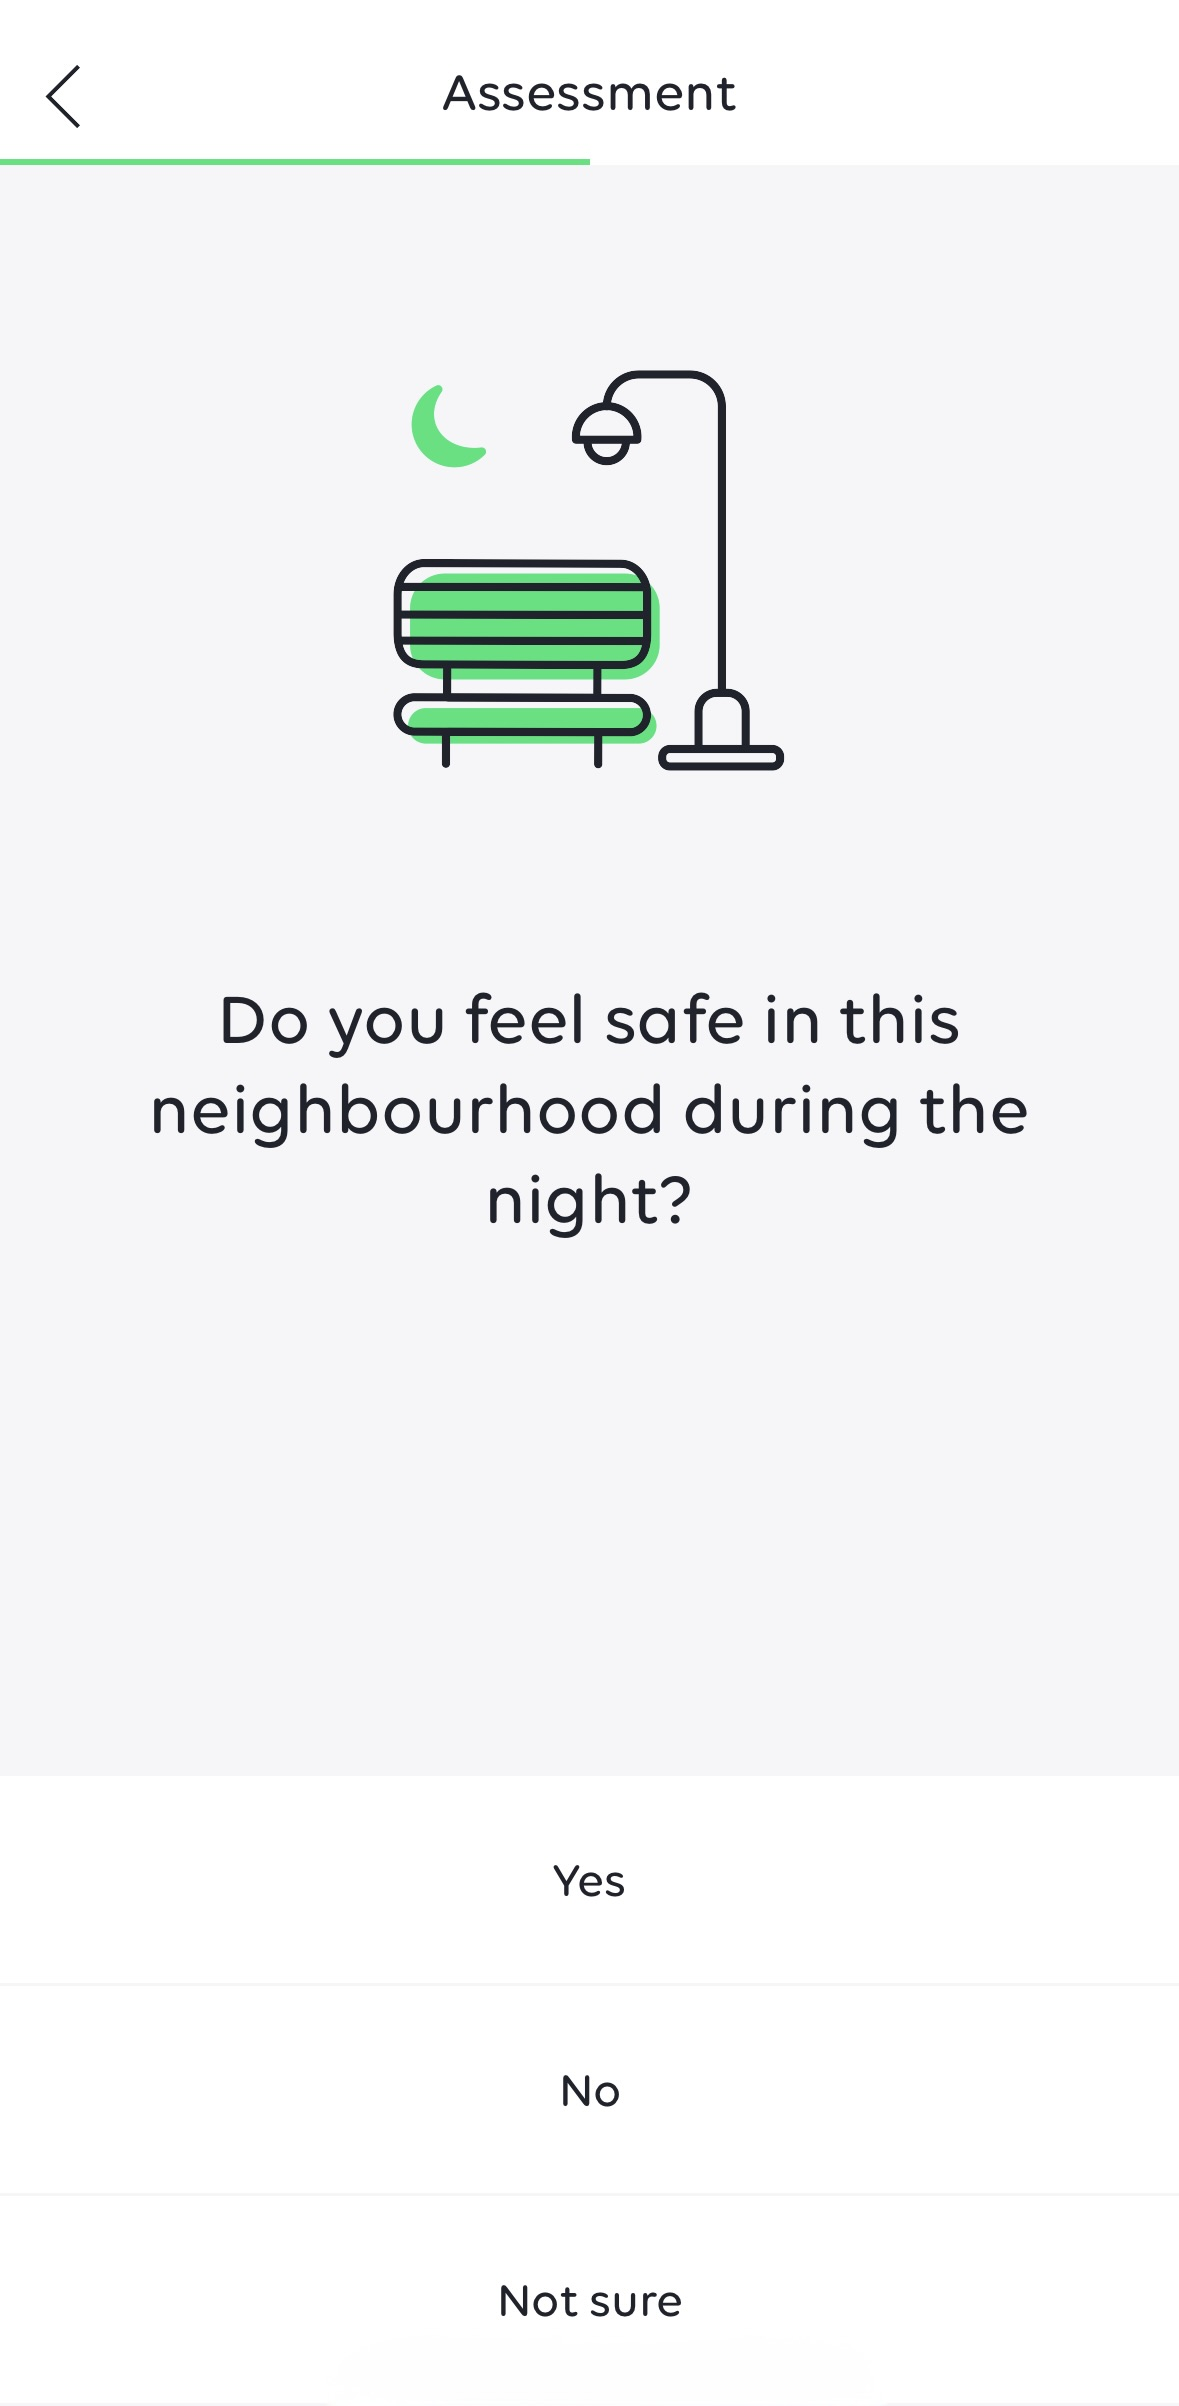
\includegraphics[width=\textwidth]{Arbeit/Bilder/urban_mind01.jpeg}
        \caption{Screenshot einer typischen Frageseite aus der \gls{urbanmind}-App}
        \label{fig:urban_mind_screenshot_1}
    \end{minipage}
    \hspace{0.1\textwidth}
    \begin{minipage}[t]{0.38\textwidth}
        \centering
        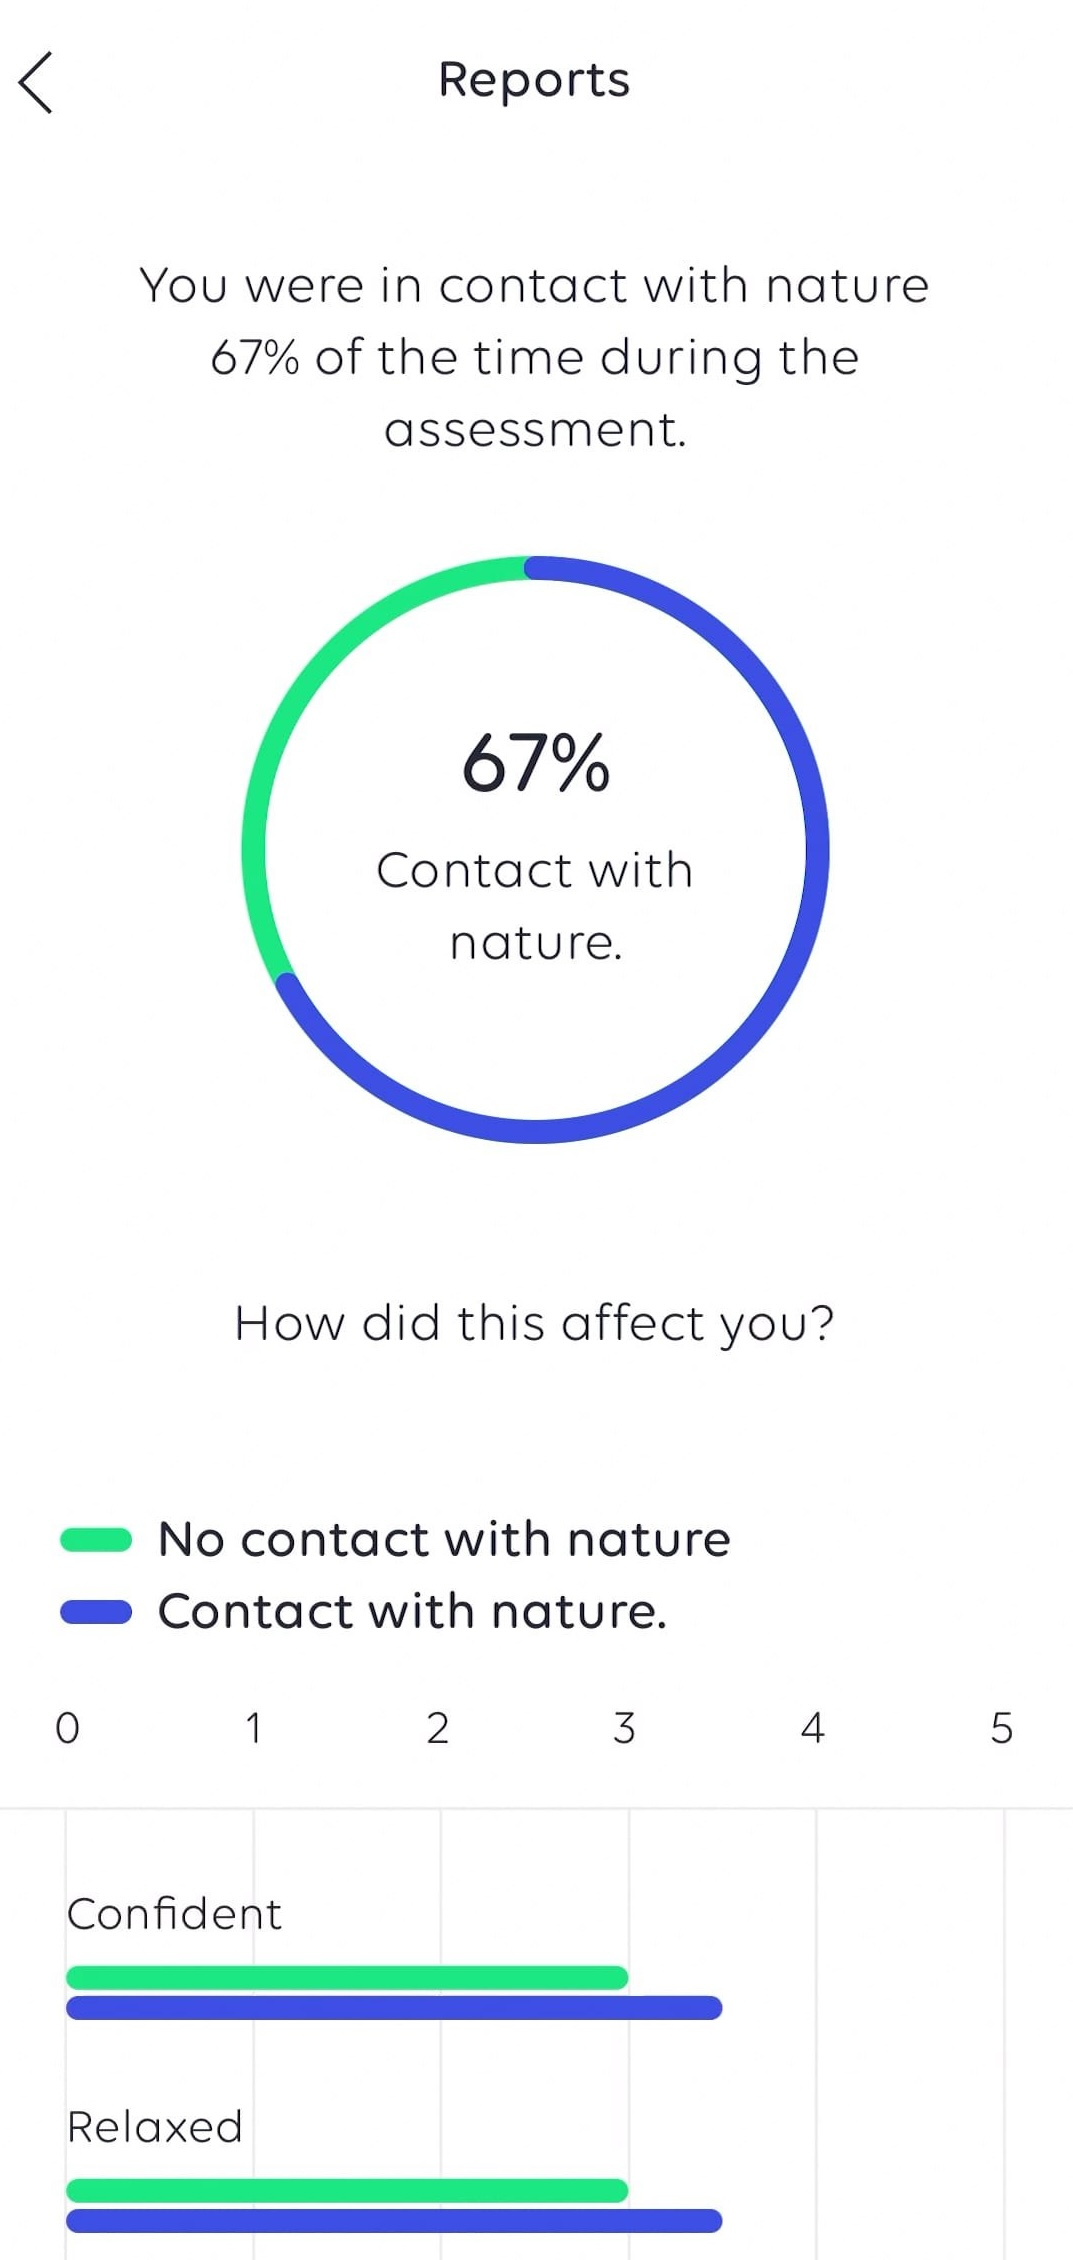
\includegraphics[width=\textwidth]{Arbeit/Bilder/urban_mind_report.jpg}
        \caption{Screenshot eines individuellen Reports aus der \gls{urbanmind}-App}
        \label{fig:urban_mind_report}
    \end{minipage}
\end{figure}

\gls{urbanmind} zeichnet sich durch eine einfache und ansprechend gestaltete Benutzeroberfläche aus, die eine niedrige Einstiegshürde für die Teilnehmenden bietet (siehe \cref{fig:urban_mind_screenshot_1}). Im Mittelpunkt stehen kurze Befragungen, die jeweils etwa drei Minuten dauern und die Teilnehmenden abhängig von der konkreten Studie \gls{bspw} zu ihrem momentanen Wohlbefinden, aktuellen Tätigkeiten sowie ihrer direkten räumlichen und sozialen Umgebung befragen. Diese Befragungen werden in den meisten Studien drei Mal täglich über eine Dauer von zwei Wochen durchgeführt. Teilnehmende werden dazu jeweils mit einer Push-Mittielung benachrichtigt und haben anschliessend jeweils eine Stunde Zeit, um die Befragung abzuschliessen.

Zusätzlich zu den standardisierten Fragebogen-Items erfasst die App kontinuierlich im Hintergrund Standortdaten mittels \gls{gps} sowie optional Gesundheits- und Aktivitätsdaten (\gls{zb} Schrittzahl, zurückgelegte Distanzen), sofern die Teilnehmenden diese Datenerfassung explizit freigeben. Weiter bietet \gls{urbanmind} die Möglichkeit, kurze Audioaufnahmen und Fotos zu teilen. Diese Mediendateien werden nicht nur für wissenschaftliche Analysen, sondern auch für künstlerische Zwecke und Öffentlichkeitsarbeit verwendet \parencite{UrbanMindPrivacy}.

Diese Praxis wirft kritische Fragen hinsichtlich Datenschutz und informierter Einwilligung auf -- insbesondere da besonders sensible Daten wie kontinuierliche Standortverläufe und Gesundheitsinformationen betroffen sind. Hinzu kommt, dass die Teilnehmenden ihre Zustimmung nicht differenziert nach Verwendungszweck (\gls{zb} Forschung, Kunst, Social Media) geben können, sondern pauschal für alle vorgesehenen Nutzungen. Informationen zur tatsächlichen Verwendung der Daten sind zudem nicht durchgängig transparent oder direkt in der App zugänglich, sondern teilweise nur über ergänzende Webseiten auffindbar.

Eine Besonderheit der App sind individuelle Reports, die Teilnehmenden automatisch und übersichtlich Rückmeldungen über ihre Interaktionen mit der Umwelt geben. So wird \gls{bspw} am Ende der Studiendauer dargestellt, bei wie vielen Befragungen die Teilnehmenden in Kontakt mit Natur waren und wie sich dies auf verschiedene Aspekte des persönlichen Wohlbefindens auswirkte (siehe \Cref{fig:urban_mind_report}). Dies dient sowohl der Reflexion über das eigene Alltagsverhalten als auch der Motivation, längerfristig an der Studie teilzunehmen.

Trotz seiner vielseitigen und benutzerfreundlichen Gestaltung weist \gls{urbanmind} einige Einschränkungen auf: Teilnehmende haben \gls{bspw} keine Möglichkeit, ihre erhobenen Rohdaten direkt zu exportieren, und auch die Löschung persönlicher Daten erfordert den expliziten Kontakt mit dem jeweiligen Forschungsteam. Entscheidend ist jedoch, dass der Quellcode der App nicht öffentlich zugänglich ist – eine unabhängige Prüfung oder Weiterentwicklung der technischen Infrastruktur bleibt damit ausgeschlossen.

Ich sehe in diesem Mangel an Transparenz und Offenheit eine Lücke im bestehenden Tool-Ökosystem -- er bildet deshalb einen wesentlichen Ausgangspunkt für die hier entwickelte App \gls[noindex]{intermind}.

\subsection*{Relief Maps+: Reflexive und intersektionale Kartierung retrospektiver Erfahrungen}

Im Unterschied zu \gls{urbanmind} verfolgen \gls{reliefmaps}\footnote{\href{https://reliefmaps.upf.edu/}{reliefmaps.upf.edu}} einen qualitativ-reflexiven Ansatz, der retrospektiv subjektive Erfahrungen intersektional positioniert sichtbar macht. \textcite   {rodo-de-zarateDevelopingGeographiesIntersectionality2014} entwickelt sie, um Machtachsen, Erfahrungen und konkrete Orte relational zu verbinden und so zu zeigen, wie Privilegien und Diskriminierungen situativ variieren. \citeauthor{rodo-de-zarateYoungLesbiansNegotiating2015} verdeutlicht dies am Beispiel \emph{junger} \emph{lesbischer} \emph{Frauen}: Durch die Kartierung ihrer Alltagswege und -Orte wird sichtbar, wie öffentliche Räume als \enquote{Orte der Unterdrückung} oder \enquote{Orte der Erleichterung} erfahren werden -- etwa wenn Blicke, Anfeindungen oder die Präsenz bestimmter Gruppen Unsicherheit hervorrufen, während andere Kontexte Zugehörigkeit und Sicherheit ermöglichen \parencite{rodo-de-zarateYoungLesbiansNegotiating2015}. 

\textcite{rodo-de-zarateIntersectionalitySpatialityEmotions2023} entwickelt den Ansatz weiter, indem sie Emotionen explizit als analytische Dimension integriert. Gefühle wie Angst, Sicherheit oder Freude erscheinen dabei nicht als rein individuelle Zustände, sondern als räumlich situierte Marker, über die Machtverhältnisse affektiv vermittelt werden. Anhand qualitativer Interviews und der Verortung emotionaler Erfahrungen in Relief Maps zeigt sie, wie Ungleichheiten nicht nur strukturell, sondern auch leiblich-situativ erfahrbar sind. Der Ansatz lässt sich damit als Werkzeug an den Rändern klassischer \gls{gis}-Traditionen einordnen, das weniger metrische Genauigkeit anstrebt, sondern alternative Formen des Mappings eröffnet, um subjektive Erfahrungen und soziale Relationen sichtbar zu machen \parencite{font-casasecaMarginsGeographicalInformation2024}.

Zu Beginn des Erhebungsprozesses erstellen Nutzer\genderstern innen einen Avatar auf Basis intersektional relevanter Merkmale wie \emph{Geschlecht}, \emph{Sexualität}, \gls{class}, \emph{Herkunft}, \emph{Körperbild} oder \emph{(Dis-)Ability}. Darauf aufbauend reflektieren sie in mehreren Schritten über Erfahrungen in verschiedenen Raumkategorien wie \enquote{öffentliche Räume}, \enquote{Gesundheitseinrichtungen} oder \enquote{virtuelle Räume} (siehe \cref{fig:relief_maps_plus_screenshot_1}). Für jede \glslink[noindex]{identitaetsachse}{Achse} sozialer Positionierung können in einem nächsten Schritt Orte je nach erfahrenem (Un\nobreakdash"=)Wohlsein als unterdrückend, kontrovers, neutral oder entlastend klassifiziert werden. Ergänzend können Orte direkt auf einer Karte verortet und mit freien Kommentaren sowie Emotionslabels wie \enquote{Angst}, \enquote{Sicherheit} oder \enquote{Empowerment} versehen werden. Diese Funktion fördert eine dichte, kontextualisierte Beschreibung subjektiver Erlebnisse, die sich nicht auf standardisierte Itemskalen reduzieren lässt.

\begin{figure}[htbp]
    \centering
    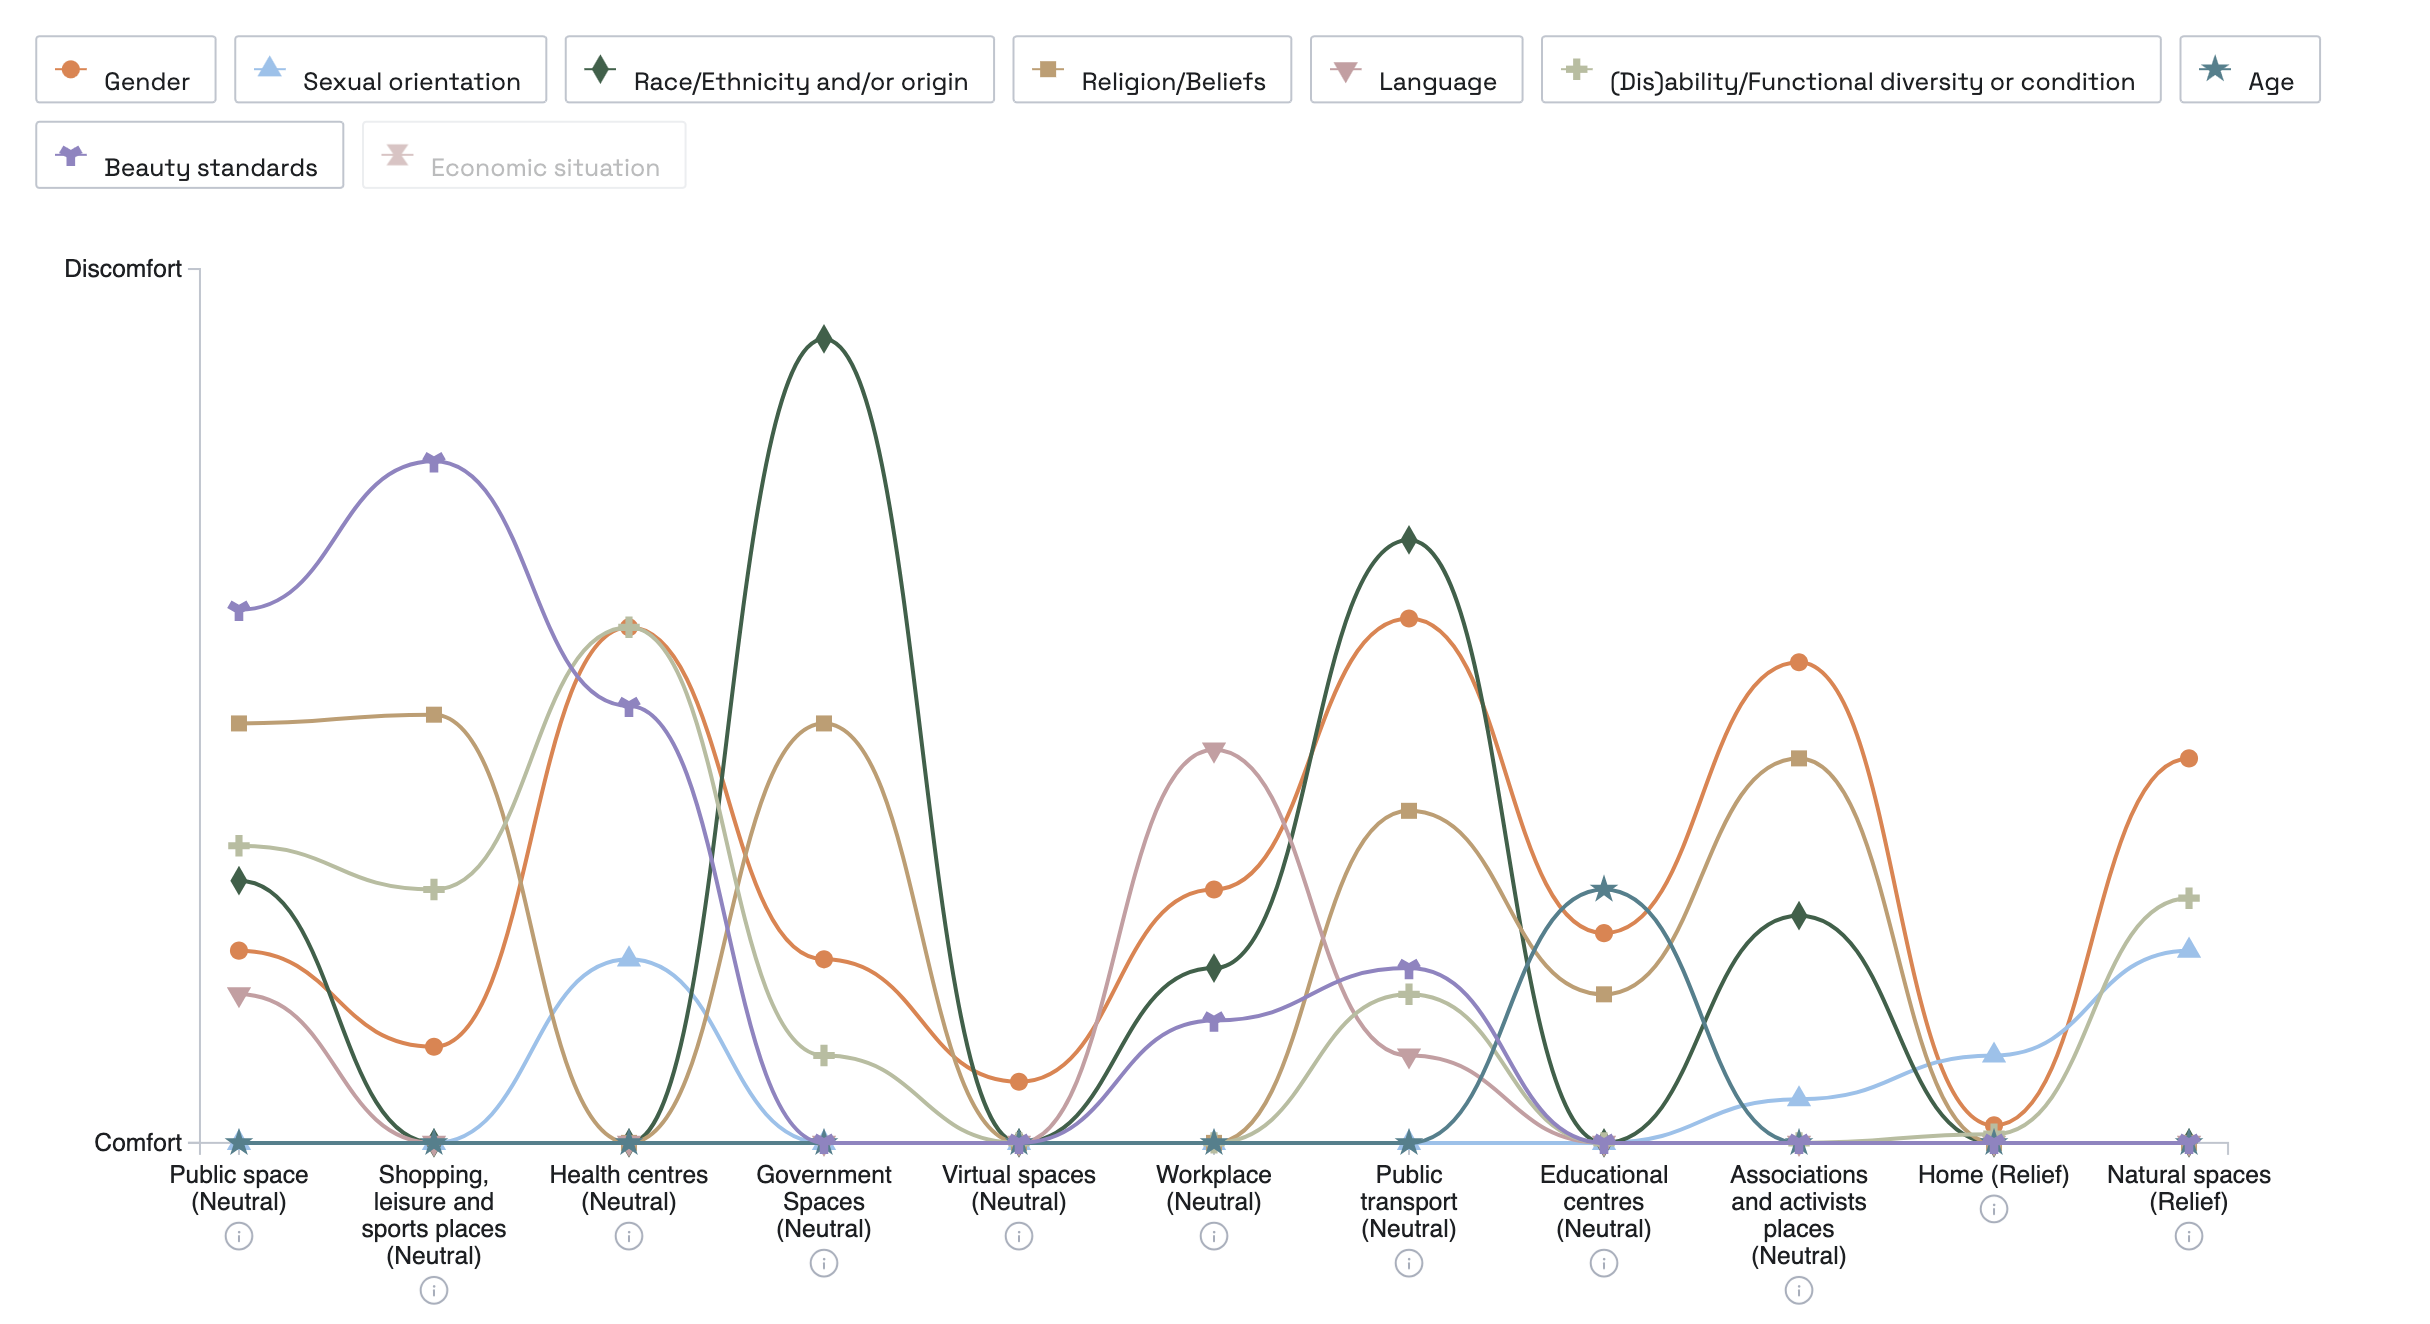
\includegraphics[width=\textwidth]{Arbeit/Bilder/reliefmap.png}
    \caption{Ausschnitt aus einer beispielhaften Relief Map}
    \label{fig:relief_maps_plus_screenshot_1}
\end{figure}

Zentrales methodisches Merkmal von \gls{reliefmaps} ist der Versuch, die emotionale Wirkung sozialer Machtverhältnisse darstellbar zu machen -- ohne diese in eindimensionale Kausalbeziehungen zu überführen. Nutzer\genderstern innen bewerten ihre Erfahrungen explizit entlang einzelner \glspl{identitaetsachse}. Gleichzeitig zeigt sich hier eine zentrale methodologische Spannung: Die isolierte Betrachtung einzelner \glslink[noindex]{identitaetsachse}{Diskriminierungsachsen} widerspricht dem Grundgedanken einer \glslink[noindex]{intersektionalitaet}{intersektionaler} Analyse, der gerade auf die Verwobenheit und Gleichzeitigkeit verschiedener Machtverhältnisse verweist. Eine konsequente \glslink[noindex]{intersektionalitaet}{intersektionale} Operationalisierung bleibt damit methodisch herausfordernd.

Einige technische Merkmale von \gls{reliefmaps} sind auch im Hinblick auf die Entwicklung von \gls[noindex]{intermind} relevant. Die browserbasierte Anwendung erlaubt es Forschenden, eigenständig Projekte zu erstellen und auszuwerten. Allerdings ist der Zugang derzeit stark auf den katalanischen Kontext zugeschnitten, da die App nur Katalanisch, Spanisch und Englisch unterstützt. Da der Quellcode nicht öffentlich zugänglich ist, bleiben Fragen zur Anpassbarkeit, Wiederverwendbarkeit und langfristigen Wartbarkeit offen. Aus methodischer Sicht stellt sich somit die Frage, inwiefern die Software übertragbar ist auf andere sprachliche, kulturelle und geografische Kontexte.

Trotz dieser Einschränkung eröffnet \gls{reliefmaps} wichtige Potenziale: Die bewusste Integration von Reflexivität, die aktive Beteiligung der Nutzer\genderstern innen an der Interpretation ihrer eigenen Erfahrungen sowie die Sichtbarmachung räumlich kontextualisierter Ungleichheiten markieren einen innovativen Zugang für \glslink[noindex]{intersektionalitaet}{intersektionale}, subjektzentrierte Geographien.


\section{Offene Infrastruktur als Gegenentwurf}
\label{sec:offene_infrastruktur_als_gegenentwurf}

Ich verstehe die im Rahmen dieser Arbeit entwickelte App \gls[noindex]{intermind} (\gls{vgl} \cref{sec:entwicklung_app}) als offene, zugängliche und flexibel einsetzbare Plattform für \glsxtrshort[noindex]{ema} und \glsxtrshort[noindex]{gema}-Studien. Ich reagiere damit auf eine zentrale Leerstelle im bestehenden Tool-Ökosystem: Beide hier vorgestellten Anwendungen sind nicht quelloffen und dadurch weder vollständig nachvollziehbar noch unabhängig weiterentwickelbar. Dies betrifft nicht nur technische Details, sondern auch grundlegende Fragen der Datenverwendung, Kontrolle und Zugänglichkeit. Vor dem Hintergrund feministisch"=digitalen Perspektive (\gls[noindex]{vgl} \cref{sec:datafeminism}) stellt \gls[noindex]{intermind} daher bewusst nicht nur einen technischen, sondern auch einen forschungsethischen Gegenentwurf dar.

\gls[noindex]{intermind} versteht sich dabei nicht als methodische Neuerfindung, sondern als infrastrukturelle Ergänzung: Bestehende methodische Ansätze werden aufgegriffen und mit einem Fokus auf Offenheit und Modularität neu zusammengesetzt. Die Offenheit der Infrastruktur ist damit nicht nur technische Eigenschaft, sondern methodischer Anspruch.

Ziel des hier entwickelten Forschungsdesigns ist es, situiertes (Un\nobreakdash-)Wohl\-be\-find\-en nicht nur als individuelle, sondern explizit als kontextuell-räumlich bedingte Erfahrungen wiederholt zu erfassen. Dieses Studiendesign bringt gegenüber querschnittbasierten Verfahren mehrere methodische Vorteile mit sich. Erstens reduziert die wiederholte intraindividuelle Erhebung Verzerrungen durch retrospektive Einschätzungen und erlaubt eine präzisere Erfassung situativer Schwankungen \parencite{randallDevelopmentTrialMobile2013}. Zweitens ermöglicht sie eine Kontrolle individueller Basisniveaus, was insbesondere für intersektionale Analysen relevant ist, die sowohl zwischen als auch innerhalb von Personen Differenzierungen vornehmen. Drittens erlaubt die Kombination von Echtzeitbefragung und intersektionaler Mehrebenenanalyse eine kontextsensitive Modellierung der Beziehungen zwischen affektivem Zustand und Umgebung im Sinne eines relationalen, ökologisch verstandenen Raumbegriffs.


\clearpage

\chapter{«Build your own tools»: Entwicklung der App Intermind}
\label{sec:entwicklung_app}

Im Zuge dieser Arbeit wurde die App \gls{intermind} entwickelt, die als technische Grundlage für pseudonymisierte \gls[noindex]{gema}-Befragungen dient. Die App und der in dieser Arbeit eingesetzte Fragenkatalog wurden parallel und iterativ konzipiert. Während dieser Abschnitt die technische Entwicklung der App dokumentiert, wird die inhaltliche Gestaltung des Fragebogens im \cref{sec:fragebogenentwicklung} erläutert. 

Der vollständig dokumentierte Quellcode der App sowie weitere kleinere Tools und Skripte die im Prozess entstanden sind, ist auf \gls[noindex]{github}\footnote{\href{https://github.com/lbatschelet/intermind}{https://github.com/lbatschelet/intermind}} unter einer AGPL-3.0-Lizenz veröffentlicht.


\section{From Scratch -- Warum eine eigene App?}
\label{sec:entwicklung_app_begruendung}

Um die Fragestellung dieser Arbeit zu bearbeiten, wurde ein Instrument benötigt, das wiederholte, geolokalisierte und kontextsensitive Erhebungen im Alltag der Teilnehmenden ermöglicht. Naheliegend wäre der Rückgriff auf bestehende und in Forschung eingesetzte Werkzeuge wie \gls{urbanmind}. Wie in \cref{sec:vergleich_bestehender_instrumente, sec:offene_infrastruktur_als_gegenentwurf} beschrieben, ist diese App aber nicht quelloffen und daher weder vollständig nachvollziehbar noch eigenständig anpassbar. Insbesondere bei der Erhebung sensibler Daten zu Wohlbefinden, sozialen Positionierungen und erlebter Diskriminierung ist eine transparente, kontrollierbare und sichere Datenverarbeitung jedoch essenziell.

Auch kommerzielle Lösungen wie die Marktforschungsplattform \textit{Avicenna}\footnote{\href{https://avicennaresearch.com/}{https://avicennaresearch.com/}} kommen nicht infrage -- neben hohen Lizenzkosten bieten auch sie nur eingeschränkte Anpassungs- und Kontrollmöglichkeiten und erfüllen zentrale ethische Anforderungen nicht.

Aus dieser Analyse ergibt sich die Notwendigkeit, ein eigenes Erhebungstool zu entwickeln, das diesen Anforderungen gerecht wird. Die Anwendung soll mobil und einfach nutzbar sein, Antworten im situativen Alltag der Teilnehmenden ermöglichen und Standortdaten automatisch erfassen. Dabei sollen datenschutzrechtliche und technische Hürden möglichst gering gehalten und die Umsetzung im Rahmen dieser Arbeit realisierbar sein.
Gleichzeitig soll sie so flexibel und nachhaltig gestaltet sein, dass Fragenkataloge, Inhalte und Erhebungslogik für zukünftige Forschungsvorhaben problemlos angepasst werden können.

Die Entscheidung zur Entwicklung eines eigenen Erhebungstools ist daher nicht nur technisch motiviert, sondern folgt auch einer forschungsethischen Logik: Wie im \cref{sec:datafeminism} dargelegt, sind digitale Infrastrukturen nie neutral, sondern Ausdruck gesellschaftlicher Machtverhältnisse. Eine transparente und kontrollierbare Datenverarbeitung ist insbesondere dann zentral, wenn -- wie im vorliegenden Projekt -- sensible Informationen zu Wohlbefinden, sozialer Zugehörigkeit und Diskriminierung erhoben werden. Die Entscheidung für eine \gls[noindex]{opensource}-Architektur ist dabei Ausdruck eines bewussten Gestaltungswillens im Sinne digitaler Souveränität: Die gesamte Infrastruktur soll nachvollziehbar, anpassbar und kollektiv weiterentwickelbar bleiben, um technologische Gestaltungsmacht nicht an proprietäre Systeme abzugeben, sondern sie partizipativ zurückzugewinnen.

\section{Konzeption und Anforderungen -- Der Weg zur eigenen Infrastruktur}
\label{sec:app_entwicklung_anforderungen}

Auf Basis der beschriebenen Anforderungen wurde zunächst ein detaillierter Anforderungskatalog entwickelt, der als zentraler Leitfaden für die weiteren Schritte der Entwicklung diente. Dieser Katalog wurde iterativ ergänzt, konkretisiert und während des gesamten Entwicklungsprozesses kontinuierlich an methodische und technische Erkenntnisse angepasst. Die Klassifikation der Anforderungen erfolgt orientiert an der in der Softwareentwicklung üblichen Unterscheidung zwischen funktionalen und nicht-funktionalen Anforderungen.

Funktionale Anforderungen definieren konkret, \textit{was} die App leisten muss, und legen somit die notwendigen Funktionen und Abläufe der Anwendung fest. Für diese Anwendung bedeutet dies insbesondere, dass die App den Teilnehmenden täglich mehrere zufällig verteilte Zeitfenster zur Beantwortung von Fragen ermittelt und jeweils zu Beginn dieser Zeiträume \glspl{pushnotification} sendet. Da gängige Webbrowser keine verlässlichen Push-Benachrichtigungen oder zeitgesteuerten Hintergrundprozesse erlauben, schliesst diese Anforderung eine browserbasierte Erhebung aus und führt zur Entscheidung für eine App-basierte Lösung. Die App erfasst bei jeder Befragung automatisiert den aktuellen \gls{gps}-Standort. Um die Erhebung flexibel und bedarfsgerecht zu gestalten, unterstützt sie verschiedene Fragetypen -- darunter Single-Choice, Multiple-Choice, Skalen-basierte Fragen (Slider) sowie Freitextfelder. Im Sinne der Selbstbestimmung über die eigenen Daten ist es funktional zwingend vorgesehen, dass Teilnehmende sämtliche mit ihrem Gerät verknüpften Daten eigenständig und dauerhaft löschen können. Die Teilnahme erfolgt vollständig pseudonym, ohne dass eine Registrierung oder die Angabe personenbezogener Daten erforderlich ist. Darüber hinaus muss die App auf \gls{android}- und \gls{ios}-Geräten lauffähig sein, in Deutsch, Englisch und Französisch verfügbar sein und die Möglichkeit zur Erweiterung um weitere Sprachen bieten. Eine ursprünglich geplante Offlinefähigkeit wurde im Verlauf der Entwicklung verworfen, da sie zu Inkompatibilitäten bei der Aktualisierung des Fragenkatalogs geführt hätte.

Nicht-funktionale Anforderungen legen fest, \textit{wie} die oben beschriebenen Funktionen umgesetzt werden sollen, und beschreiben qualitative Merkmale wie Sicherheit, Benutzerfreundlichkeit oder technische Nachvollziehbarkeit. Zu den zentralen nicht-funktionalen Anforderungen zählen Datenschutz, Datensicherheit und technische Qualität. Sämtliche Datenverarbeitungsprozesse müssen im Einklang mit dem Schweizer Datenschutzgesetz (\glsxtrshort{dsg}) sowie der Europäischen Datenschutzgrundverordnung (\glsxtrshort{dsgvo}) erfolgen. Darüber hinaus ist sicherzustellen, dass alle Datenübertragungen verschlüsselt erfolgen und keine Dritten Zugriff auf die gespeicherten Daten erhalten. Diese Ausgestaltung folgt nicht nur rechtlichen Vorgaben, sondern knüpft auch an die im \cref{sec:datafeminism} entwickelten Prinzipien einer digitalen Souveränität an, die Transparenz, Kontrolle und Selbstbestimmung in den Mittelpunkt stellt. Eine offene, modulare und nachvollziehbare Codebasis soll gewährleisten, dass Anpassungen und Erweiterungen des Systems durch andere Forschende mit minimalem Aufwand möglich sind. Dies wurde durch die Veröffentlichung der App als \gls{opensource}-Projekt auf \gls{github} umgesetzt.

Zur systematischen Umsetzung der Anforderungen wird ein iterativer Entwicklungsprozess auf Basis von \glspl{githubissue} genutzt, in dem jede funktionale und nicht-funktionale Anforderung als eigenes \glslink{githubissue}{Issue} dokumentiert und mit einem Meilenstein versehen ist, der den geplanten Umsetzungszeitpunkt markiert. Diese Meilensteine orientieren sich an vier Entwicklungsstufen: Als \textit{core \glsxtrfull{mvp}} wird die minimal funktionsfähige Version der App bezeichnet, die alle für die Durchführung der Studie zwingend notwendigen Funktionen enthält, wie etwa die zeitgesteuerte Versendung von \glspl{pushnotification}, die Erfassung des \gls{gps}-Standorts oder die Bereitstellung zentraler Fragetypen. Das \textit{extended \gls{mvp}} umfasst zusätzliche Funktionen, die den Erhebungsprozess verbessern, für die Beantwortung der Forschungsfrage jedoch nicht zwingend erforderlich sind, beispielsweise die Unterstützung mehrerer Sprachen oder zusätzliche Fragetypen. Der Meilenstein \textit{app store release} umfasst alle Aufgaben, die für die Veröffentlichung in App-Stores erforderlich sind, jedoch keinen direkten Einfluss auf die eigentliche Datenerhebung oder Kernfunktionen der App haben. Dazu zählen begleitende Arbeiten wie die Erstellung einer Projektwebsite mit Datenschutzrichtlinie, die Bereitstellung der für die App-Store-Einreichung notwendigen Assets, die Einrichtung einer kontinuierlichen Integrations- und Auslieferungspipeline (\gls{cicd}) sowie die Durchführung des formalen Prüf- und Freigabeprozesses der App-Stores. Unter \textit{future enhancements} werden schliesslich langfristig geplante Erweiterungen verstanden, die den Funktionsumfang der App über die Anforderungen der vorliegenden Arbeit hinaus erweitern. Derzeit stehen hier vor allem eine Offlinefähigkeit der App sowie die Möglichkeit einer direkten Auswertung der erhobenen Daten innerhalb der App auf der Liste, wobei noch offen ist, ob und in welchem Umfang diese Funktionen umgesetzt werden. Die Priorisierung innerhalb dieser Kategorien orientiert sich an den Forschungszielen, den rechtlichen Vorgaben, der technischen Machbarkeit sowie den in \cref{sec:datafeminism} ausgeführten Prinzipien, wobei Änderungen am Funktionsumfang während der Entwicklung fortlaufend in den entsprechenden \glslink{githubissue}{Issues} dokumentiert werden.


\section{Technische Umsetzung -- Prinzipien, Praktiken und Kompromisse}
\label{sec:app_entwicklung_technische_umsetzung}

Die technische Umsetzung folgt etablierten Prinzipien der Softwareentwicklung, insbesondere \textit{Privacy by Design} \parencite{cavoukianPrivacyDesign72009} und den Gestaltungsprinzipien von \gls{solid} \parencite{martinCleanArchitectureCraftsmans2018}. Ziel ist eine modulare, wartbare und erweiterbare Architektur, die funktionale Anforderungen effizient umsetzt und nicht-funktionale Anforderungen -- insbesondere Datenschutz und Sicherheit -- von Beginn an integriert. Dabei wird eine klare Trennung zwischen Anwendungslogik, Datenhaltung und Benutzeroberfläche konsequent umgesetzt, um spätere Anpassungen und Erweiterungen mit minimalem Eingriff in bestehende Komponenten zu ermöglichen.

Für die Entwicklung der mobilen Anwendung wurde \gls{reactnative} in Kombination mit \gls{expo} gewählt. \gls{reactnative} ist ein von \gls{meta} entwickeltes, \gls{opensource} \gls{framework}, das die Entwicklung plattformübergreifender Anwendungen mit einer einzigen Codebasis ermöglicht. Dadurch können \gls{ios}- und \gls{android}-Versionen parallel gepflegt werden, was den Entwicklungs- und Wartungsaufwand erheblich reduziert. Obwohl React Native ursprünglich von einem grossen Technologiekonzern stammt, erfolgt in diesem Projekt keinerlei Datenaustausch mit \gls{meta}, da ausschliesslich das in der Entwicklungsumgebung installierte Framework verwendet wird, das weder auf den Endgeräten der Teilnehmenden noch auf externen Servern von \gls{meta} ausgeführt wird.

\gls{expo} ergänzt React Native um eine ebenfalls \gls{opensource} integrierte Entwicklungsumgebung mit Werkzeugen für Build, Test und Veröffentlichung. Dies erlaubt es, zentrale Infrastrukturaufgaben ohne eigenes \gls{devops}-Team effizient umzusetzen. Insbesondere die Möglichkeit, native Funktionen wie Push-Benachrichtigungen, Kamera- oder Standortzugriff über ein einheitliches API zu nutzen, beschleunigt die Umsetzung und reduziert die Komplexität der Codebasis. 

Als serverseitige Infrastruktur kommt \gls{supabase} zum Einsatz -- ein \gls{opensource} \gls{backend}-as-a-Service auf Basis von \gls{postgresql}, das Authentifizierung, Autorisierung, Datenspeicherung und Schnittstellenbereitstellung integriert. Die Entscheidung für Supabase erfolgte bewusst gegen den Einsatz von \gls{firebase}, das als De-facto-Standard für mobile Anwendungen gilt und in vielen Bereichen eine einfachere Implementierung ermöglicht hätte. Firebase ist jedoch ein proprietärer Dienst von \gls{google}, der zentrale Kontrolle über die Infrastruktur ausübt, den Serverstandort nicht frei wählen lässt und potenziell die Datenhoheit der Forschenden einschränkt. Wie in \cref{sec:datafeminism} ausgeführt, stehen solche zentralistischen Strukturen im Widerspruch zu Prinzipien digitaler Souveränität. Supabase ermöglicht hingegen, den Standort des Servers (hier: Schweiz) festzulegen und bietet die Option eines vollständig selbstverwalteten Betriebs. Neben der offenen Lizenz und der SQL-basierten Datenstruktur war auch die Möglichkeit eines kostenlosen Hostings für kleine Projekte ausschlaggebend, wodurch der Betrieb ohne zusätzliche Infrastrukturkosten möglich ist. Die Wahl dieser Toolchain stellt damit einen pragmatischen Kompromiss dar: Sie bietet die notwendige technische Leistungsfähigkeit und Flexibilität, ohne die Kontrolle über Daten an externe Plattformanbieter abzugeben.

\begin{figure}[h]
    \centering
    \begin{minipage}[t]{0.38\textwidth}
        \centering
        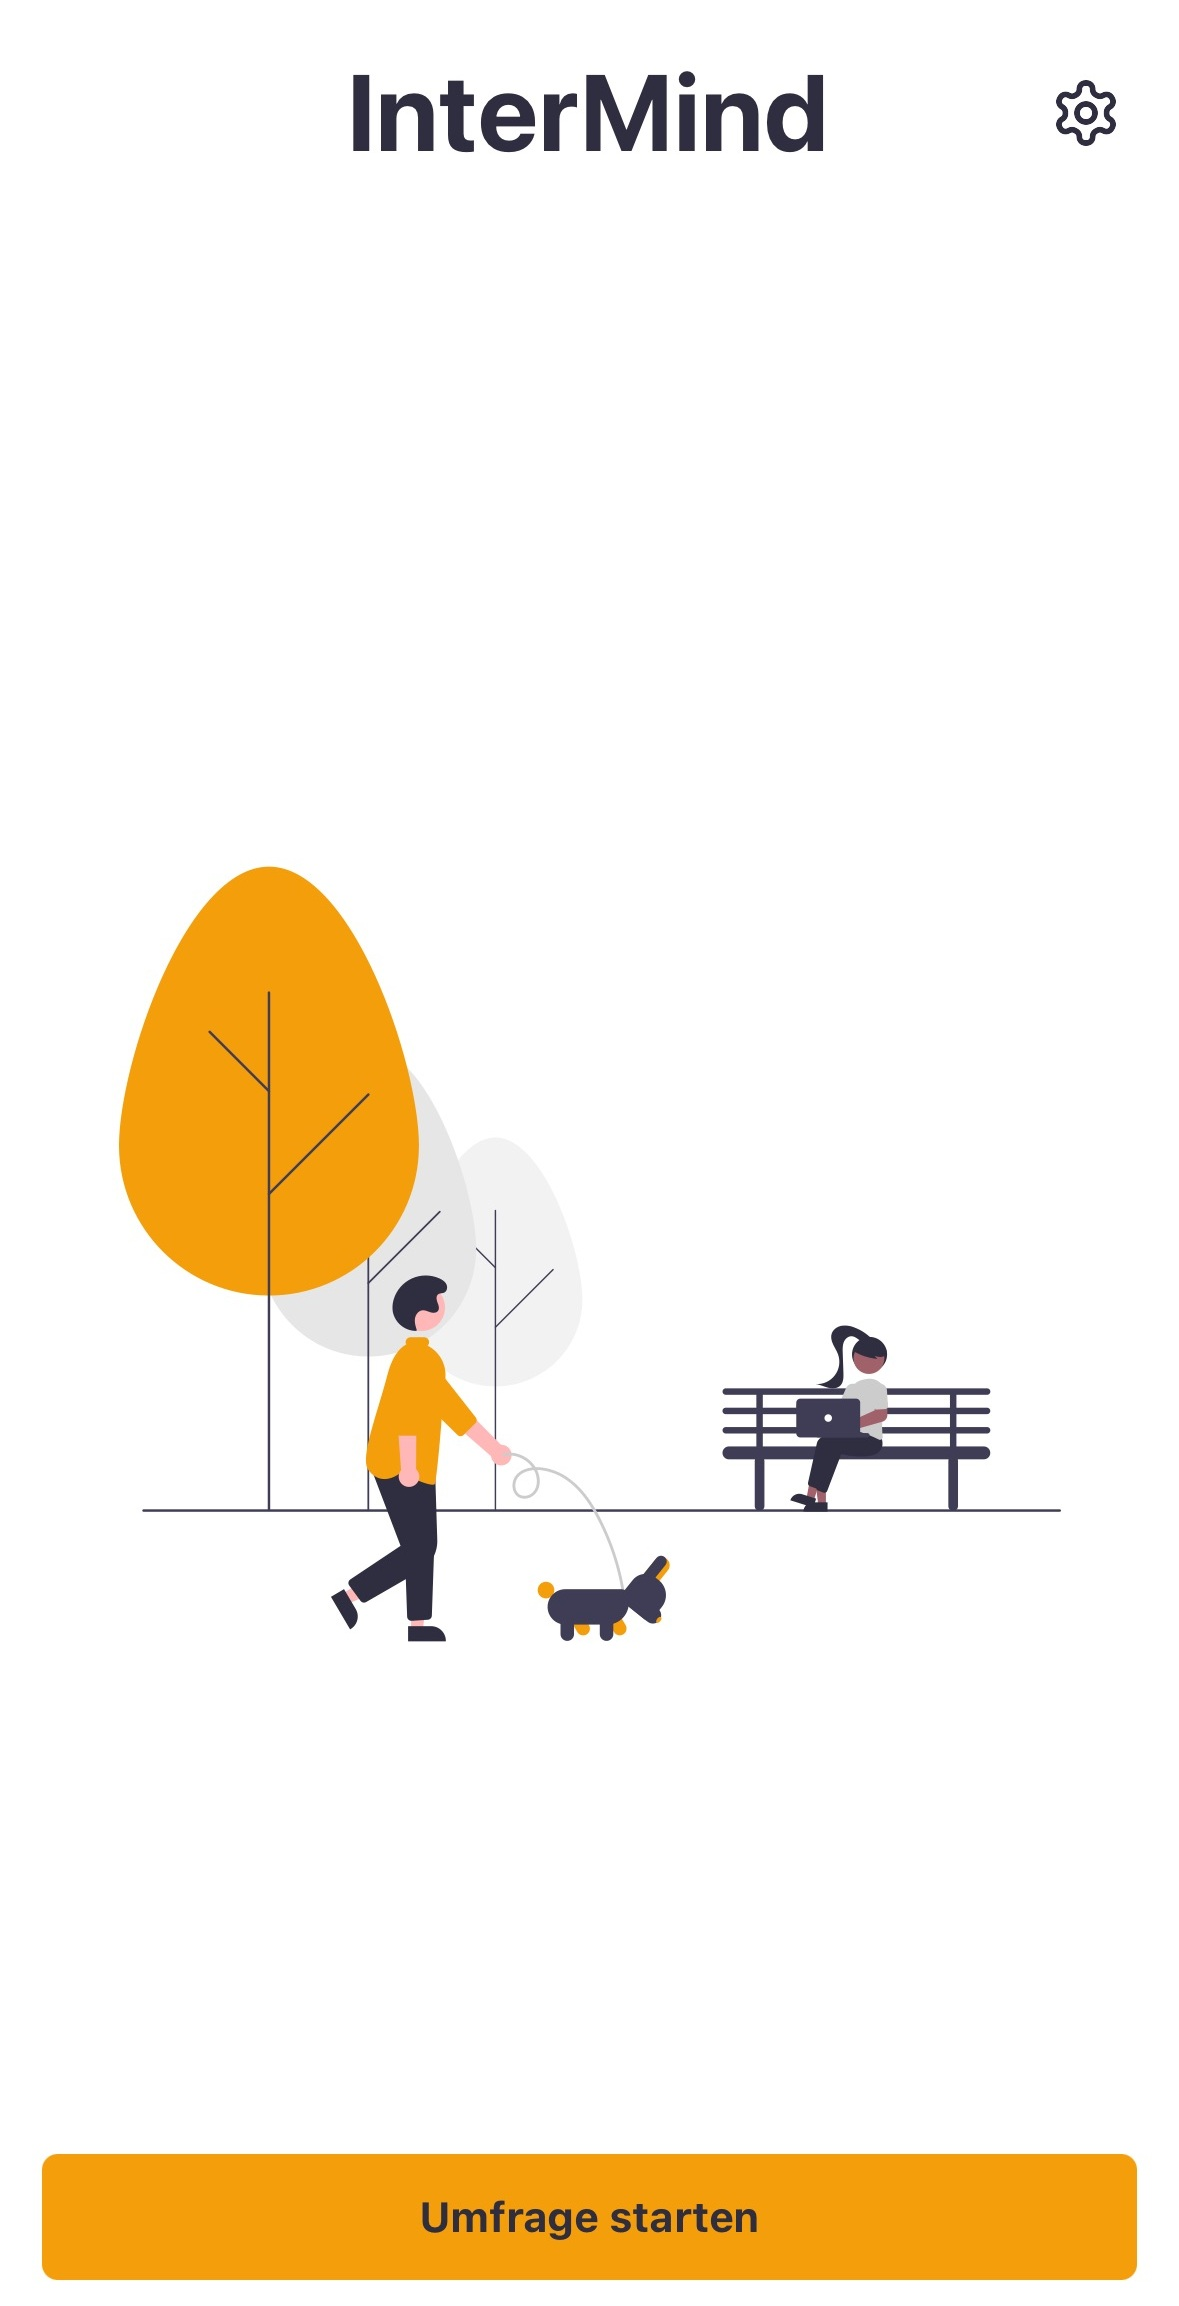
\includegraphics[width=\textwidth]{Arbeit/Bilder/printscreens/startscreen.jpeg}
        \caption{Startbildschirm der App \gls[noindex]{intermind}}
        \label{fig:startscreen}
    \end{minipage}
    \hspace{0.1\textwidth}
    \begin{minipage}[t]{0.38\textwidth}
        \centering
        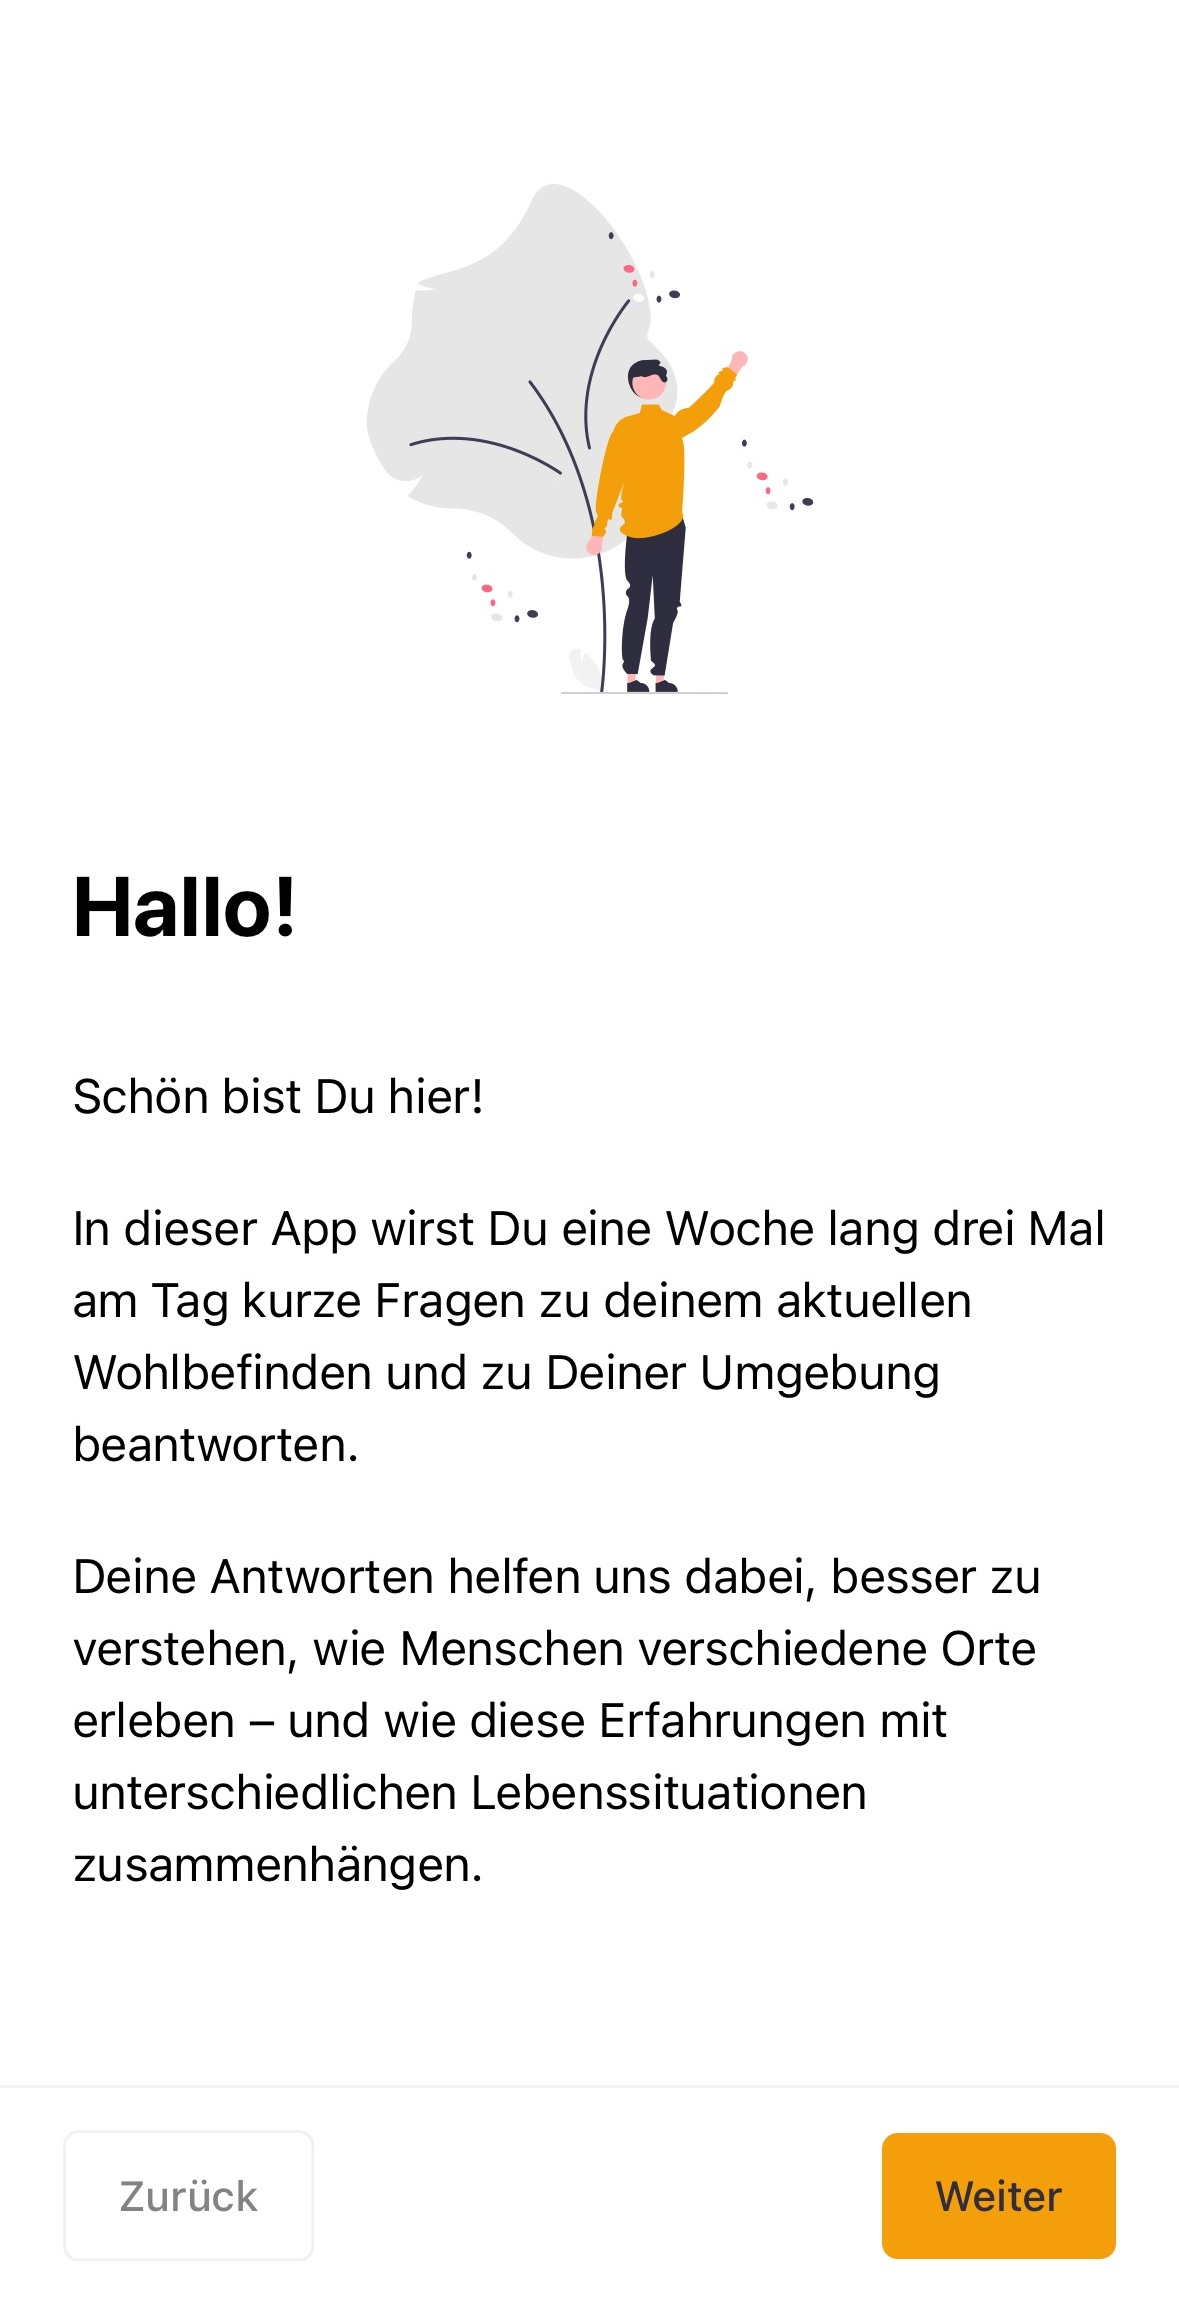
\includegraphics[width=\textwidth]{Arbeit/Bilder/printscreens/welcome.jpeg}
        \caption{Begrüssungstext der App \gls[noindex]{intermind}}
        \label{fig:welcome}
    \end{minipage}
\end{figure}

Der Quellcode folgt einer komponentenbasierten Struktur, in der jede Funktion klar abgegrenzte Verantwortlichkeiten besitzt. Diese Struktur erleichtert nicht nur die Wiederverwendung bestehender Module, sondern unterstützt auch die Adaption der Anwendung für andere Forschungsprojekte mit ähnlichem methodischen Aufbau. Die konkreten Fragebögen (\gls[noindex]{vgl} \cref{sec:fragebogenentwicklung}) werden nicht im Quellcode gespeichert, sondern als \gls{json}-Konfigurationsdateien in der \gls{datenbank} hinterlegt. Die App lädt diese Inhalte dynamisch beim Start oder bei Bedarf nach, wodurch Änderungen am Fragenkatalog ohne App-Update möglich sind. Die Entscheidung für serverseitige Speicherung erhöht die Flexibilität, birgt jedoch den Nachteil, dass eine aktive Internetverbindung erforderlich ist. Auf eine vollständige Offlinefähigkeit wird bewusst verzichtet, um Inkonsistenzen zwischen verschiedenen App-Versionen zu vermeiden und stets aktuelle Inhalte bereitzustellen.

Die datenschutzbezogene Umsetzung basiert auf einer strikten Pseudonymisierung. Beim ersten Start generiert die App automatisch eine gerätegebundene \gls{uuid}, die für alle weiteren Interaktionen verwendet wird. Aus Sicht des Systems existieren damit keine individuellen Nutzer\genderstern innen, sondern ausschliesslich Geräte-IDs. Personenbezogene Daten wie Name, Telefonnummer oder E-Mail-Adresse werden nicht erhoben. Standortdaten werden ausschliesslich zum Zeitpunkt einer beantworteten Befragung erfasst. Die Löschung aller mit einer \gls{uuid} verknüpften Datensätze kann jederzeit direkt in der App ausgelöst werden und entfernt sämtliche Einträge aus der \gls{datenbank}.

Der Zugriffsschutz wird durch eine Zugriffskontrolle auf Zeilenebene (\gls{rls}) in der \gls{postgresql}-\gls{datenbank} realisiert. Jede Anfrage an den Server ist an die jeweilige \gls{uuid} gebunden; Abfragen liefern nur Datensätze, die mit dieser ID verknüpft sind. Alle Datenübertragungen zwischen App und Server erfolgen verschlüsselt über authentifizierte Schnittstellen. Die Serverinfrastruktur befindet sich physisch in der Schweiz und unterliegt damit dem Schweizer Datenschutzgesetz (\gls{dsg}); zusätzlich werden die Vorgaben der Europäischen Datenschutzgrundverordnung (\gls{dsgvo}) eingehalten. Die vollständigen Regelungen sind in einer öffentlich zugänglichen Datenschutzrichtlinie dokumentiert, die in der App sowie auf der Projektwebseite\footnote{\href{https://intermind.ch/privacy-policy.html}{https://intermind.ch/privacy-policy.html}} verfügbar ist.

\begin{figure}[h]
    \centering
    \begin{minipage}[t]{0.38\textwidth}
        \centering
        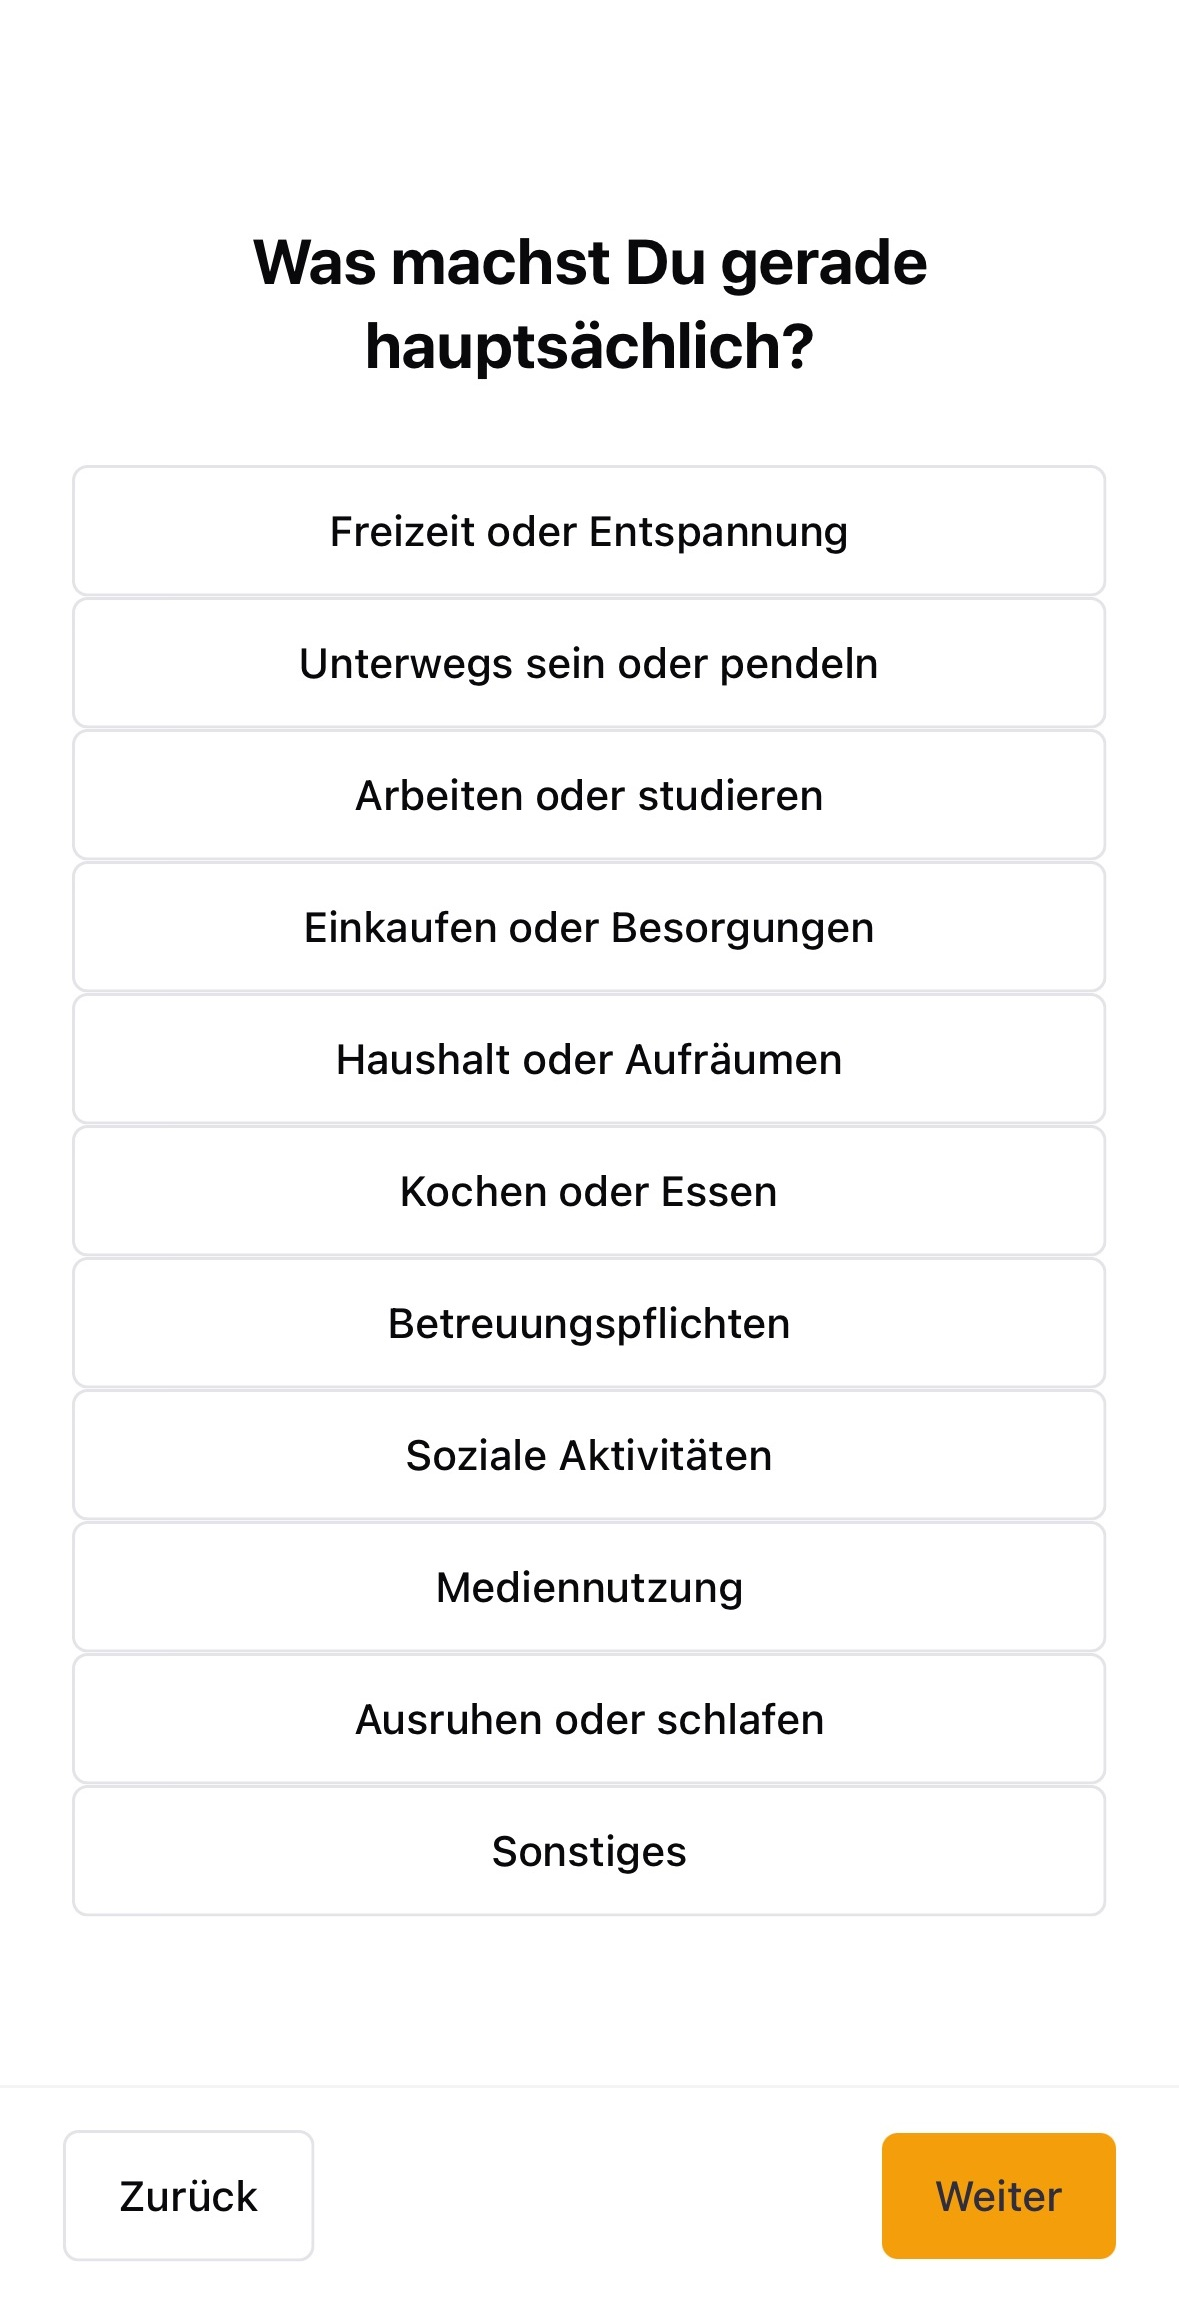
\includegraphics[width=\textwidth]{Arbeit/Bilder/printscreens/beschaeftigung.jpeg}
        \caption{Multiple-Choice-Frage zur aktuellen Beschäftigung}
        \label{fig:beschaeftigung}
    \end{minipage}
    \hspace{0.1\textwidth}
    \begin{minipage}[t]{0.38\textwidth}
        \centering
        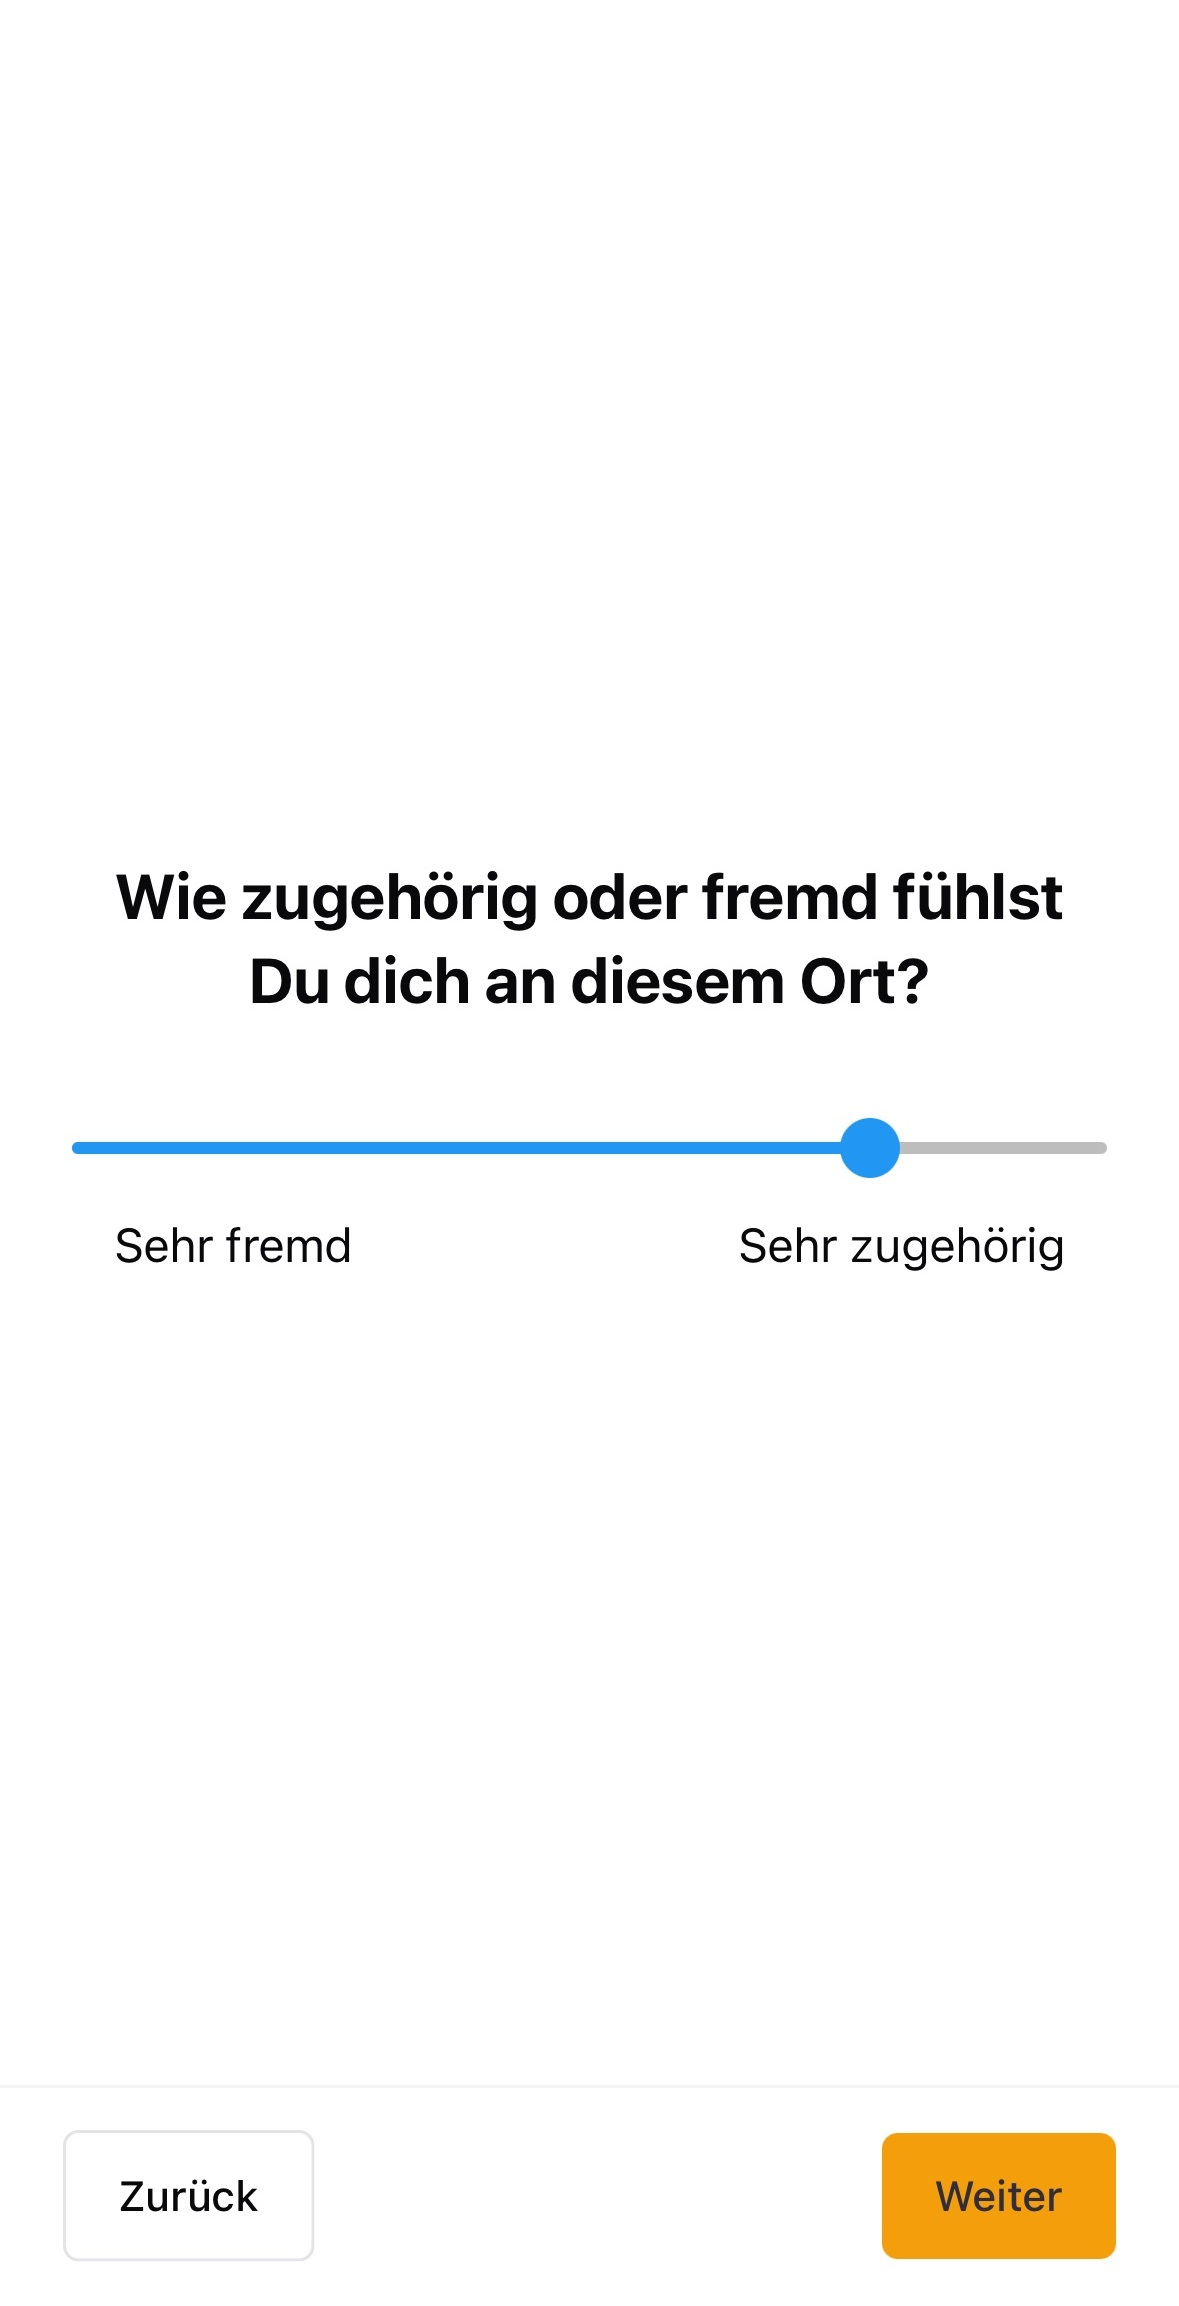
\includegraphics[width=\textwidth]{Arbeit/Bilder/printscreens/zugehoerigkeit.jpeg}
        \caption{Slider-Frage zur sozialen Zugehörigkeit}
        \label{fig:zugehoerigkeit}
    \end{minipage}
\end{figure}

Die Befragungslogik berechnet nach der ersten Teilnahme täglich drei zufällige Befragungszeitpunkte, die innerhalb fester Tagesabschnitte (Morgen, Mittag/Nachmittag, Abend) ausgewählt werden. Diese Zeitpunkte werden lokal auf dem Gerät gespeichert. Zwischen zwei Befragungen wird ein Mindestabstand von zwei Stunden eingehalten, gerechnet zwischen dem Ende des vorigen und dem Beginn des nächsten Befragungsfensters, um zu vermeiden, dass Teilnehmende bei kurzfristiger Nichtverfügbarkeit mehrere Erhebungen unmittelbar hintereinander verpassen. Zum Start eines Zeitfensters wird eine Push-Benachrichtigung versendet; der Fragebogen kann innerhalb einer Stunde beantwortet werden, danach verfällt der Slot.

Die Entscheidung für dieses Zeitplanmodell orientiert sich am Design der \textit{Urban Mind}-App \parencite{bakolisUrbanMindUsing2018}, das sich in der Praxis als gut umsetzbar erwiesen hat. Die Kombination aus zufälliger Platzierung der Startzeiten innerhalb fest definierter Tagesfenster und einer begrenzten Bearbeitungsdauer ermöglicht es, Antworten zu unterschiedlichen Zeitpunkten des Tages zu erfassen und damit Variabilität im Tagesablauf der Teilnehmenden abzubilden. Gleichzeitig wird vermieden, dass Befragungen immer zu denselben Uhrzeiten stattfinden, was potenzielle Antwortmuster verzerren könnte.

Die Eckzeiten der drei Hauptzeitfenster sind als Variablen in der Anwendung hinterlegt und können für andere Studien oder Fragebogendesigns angepasst werden. Auf diese Weise lässt sich der Befragungsrhythmus flexibel anpassen, beispielsweise indem Tagesfenster auf Grundlage individueller Angaben zu Aufsteh- und Schlafenszeiten definiert werden. Eine solche Erweiterung würde auch nicht-normative Tagesrhythmen berücksichtigen und könnte die Erreichbarkeit der Teilnehmenden weiter verbessern.

\begin{figure}[h]
    \centering
    \begin{minipage}[t]{0.38\textwidth}
        \centering
        
\includegraphics[width=\textwidth]{Arbeit/Bilder/printscreens/fragen_zu_dir.jpeg}
        \caption{Überleitungsbildschirm zu den einmaligen Fragen}
        \label{fig:ueberleitungsbildschirm}
    \end{minipage}
    \hspace{0.1\textwidth}
    \begin{minipage}[t]{0.38\textwidth}
        \centering
        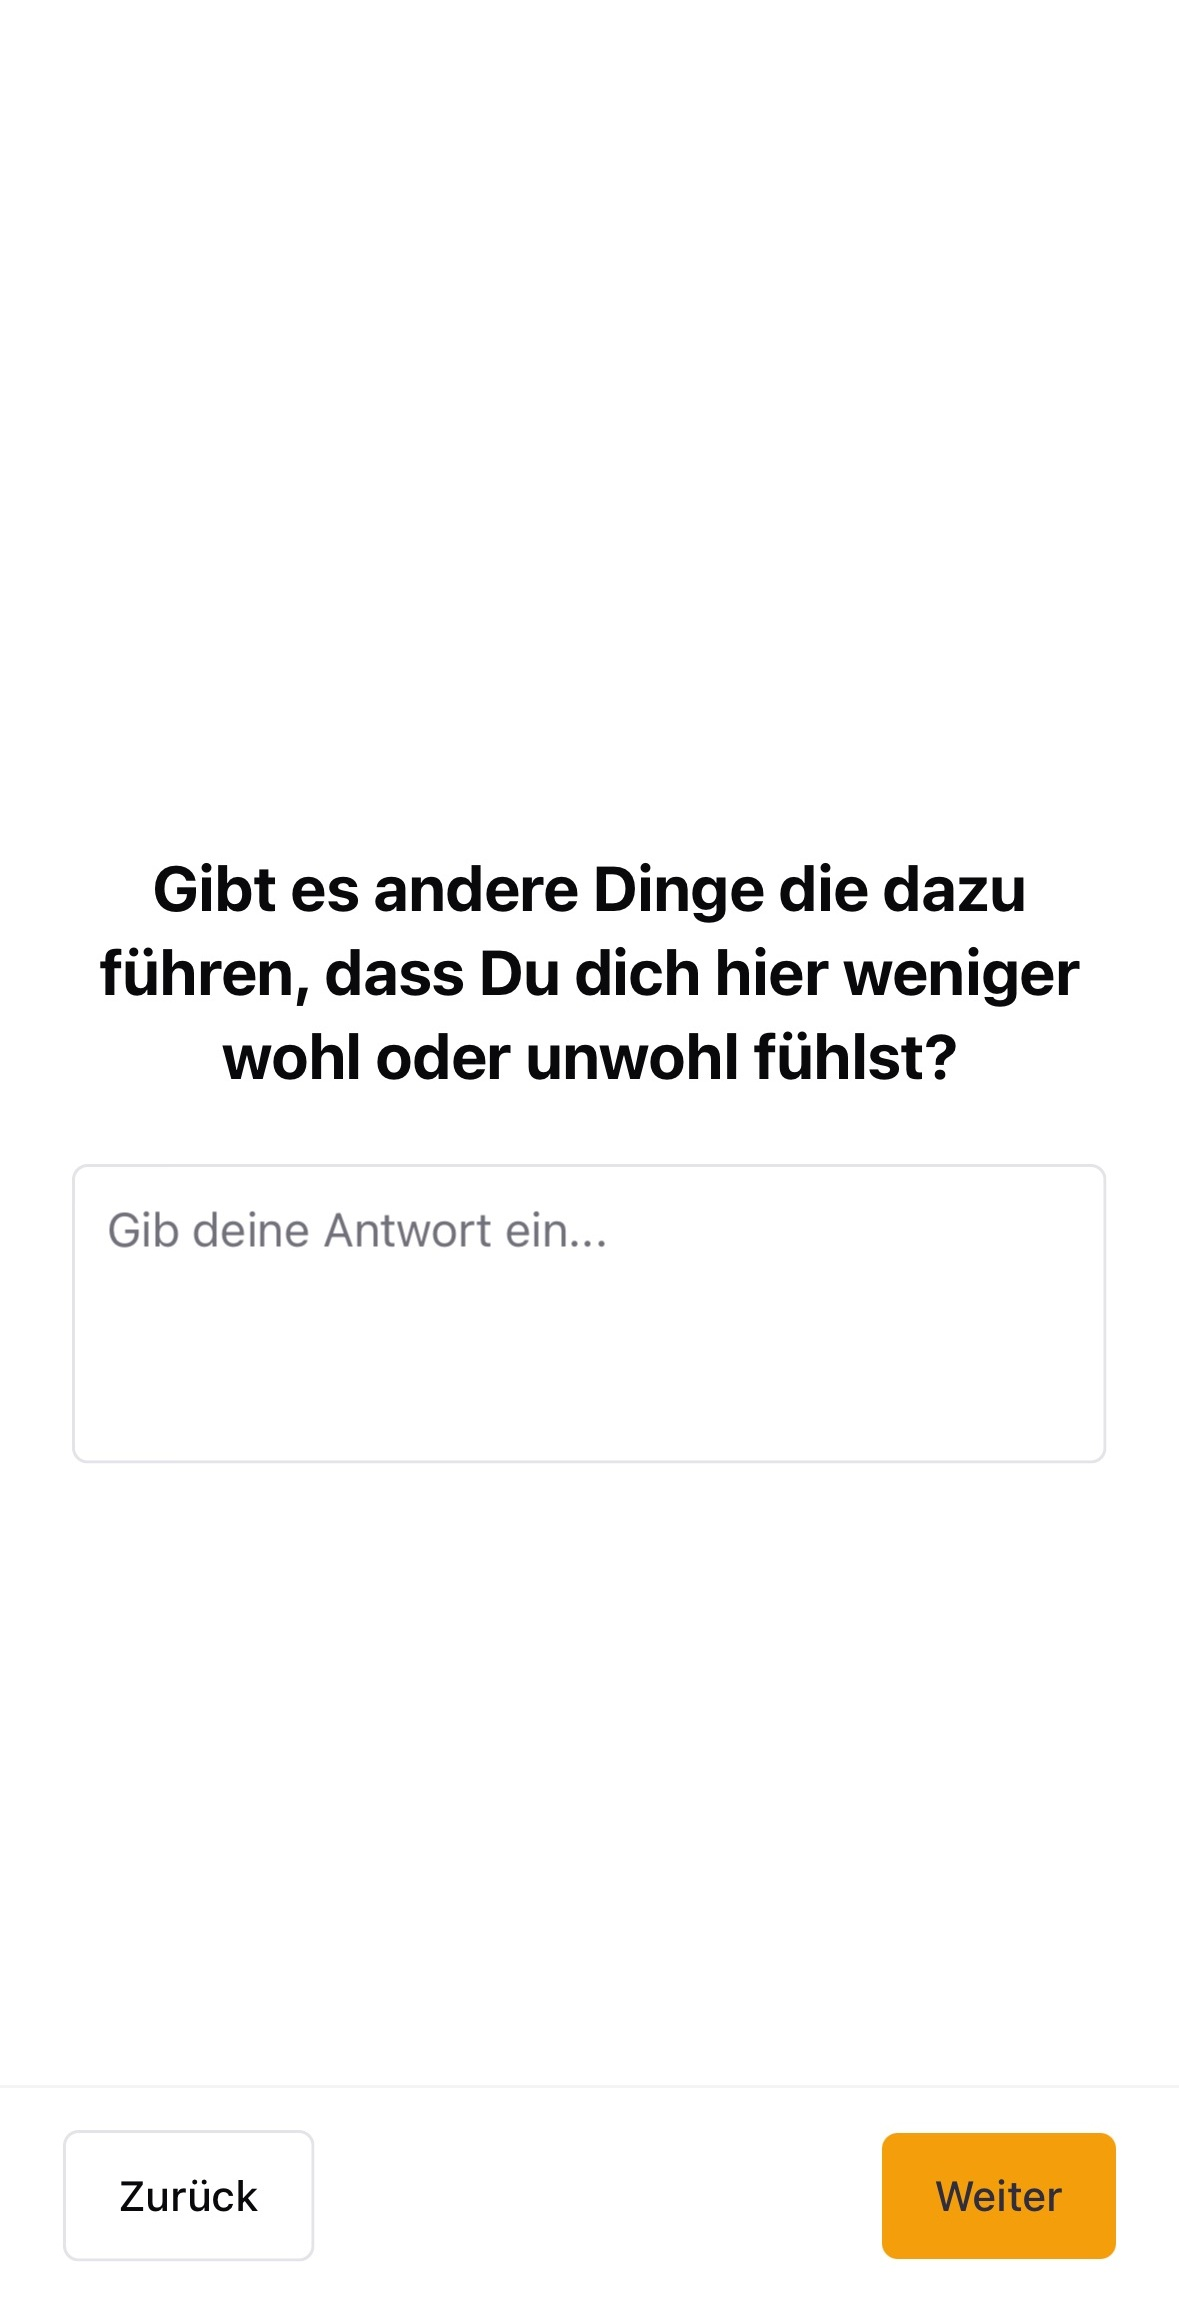
\includegraphics[width=\textwidth]{Arbeit/Bilder/printscreens/offen_unwohl.jpeg}
        \caption{Offene Textfrage zu weiteren Gründen für Unwohlsein an diesem Ort}
        \label{fig:offene_textfrage}
    \end{minipage}
\end{figure}

Die Benutzeroberfläche ist bewusst reduziert und funktional gestaltet, um eine intuitive Bedienung zu ermöglichen und die Fragen möglichst neutral darzustellen \parencite{rogersInteractionDesignHumancomputer2023}. Die App umfasst drei Hauptbereiche: den Startbildschirm (\cref{fig:startscreen}), der standardmässig den nächstmöglichen Befragungszeitpunkt prominent anzeigt und -- sofern aktuell eine Befragung verfügbar ist -- direkt einen „Umfrage starten“-Button einblendet; den Fragebogenbereich (\cref{fig:welcome,fig:beschaeftigung,fig:zugehoerigkeit,fig:ueberleitungsbildschirm,fig:offene_textfrage}), der sowohl einleitende und überleitende Texte als auch die einzelnen Fragen in einem klar strukturierten Layout präsentiert; sowie einen Informations- und Einstellungsbereich mit Hinweisen zum Datenschutz und zur Studie.

Grafiken werden ausschliesslich auf Einleitungs-, Überleitungs- und Informationsbildschirmen eingesetzt, nicht jedoch während der eigentlichen Befragung. Diese bewusste Trennung soll sicherstellen, dass die Beantwortung der Fragen nicht durch Designelemente beeinflusst wird. Für diese visuellen Elemente kommen ausschliesslich \gls{opensource}-Vektorgrafiken von Katerina Limpitsouni\footnote{\href{https://undraw.co/}{undraw.co/}} zum Einsatz, die thematisch passend, aber stilistisch neutral gehalten sind.

Die Farbpalette ist dezent gewählt, um Barrierefreiheit zu fördern und gute Lesbarkeit unter verschiedenen Lichtbedingungen sicherzustellen. Die Navigation ist linear aufgebaut: Nach Abschluss einer Befragung kehren die Nutzenden automatisch zum Startbildschirm zurück, wodurch der Fokus klar auf den nächsten Befragungszeitpunkt gelenkt wird. Komplexe Menüs oder verschachtelte Navigationsebenen werden vermieden, um die Nutzung auch für Personen mit geringer technischer Erfahrung zu erleichtern.

\section{Von der Simulation zum Alltagstest -- Feldtest und Feinschliff}
\label{sec:app_entwicklung_feldtest}

Zur Überprüfung der technischen Funktionsfähigkeit wurde ein zweistufiges Testverfahren durchgeführt: fortlaufende Tests während der Entwicklung sowie ein abschliessender interner Pretest. Auf automatisierte Tests wurde verzichtet, da deren Relevanz zu Beginn des Projekts unterschätzt und eine nachträgliche Integration als zu aufwändig eingeschätzt wurde. Stattdessen kam ein manueller, iterativer Ansatz zum Einsatz, bei dem die App regelmässig in \glspl{emulator} unterschiedlicher Bildschirmgrössen und auf physischen Geräten geprüft wurde. Die modulare Struktur der Codebasis erleichterte dabei die gezielte Überprüfung einzelner Komponenten. Im Mittelpunkt standen die dynamische Verarbeitung des Fragenkatalogs, die Datenübertragung an das \gls{supabase}-\gls{backend}, das Verhalten bei instabiler Internetverbindung sowie die Funktionsweise der lokalen Push-Benachrichtigungen.

Der anschliessende interne Pretest wurde mit vier Personen durchgeführt, die über die offiziellen Plattformen (\gls{testflight} und \gls{googleplayconsole}) Zugang zur App erhielten und diese über zwei Wochen im Alltag nutzten. Ziel war es, zentrale Funktionen unter realen Bedingungen zu überprüfen, insbesondere das Verhalten beim ersten App-Start, die Stabilität der Datenerfassung und die Darstellung auf unterschiedlichen Geräten. Rückmeldungen zur Bedienbarkeit wurden laufend dokumentiert.

Aus den Testergebnissen ergaben sich mehrere Anpassungen. Die Logik zur Planung der Slots und Benachrichtigungen wurde grundlegend überarbeitet: Anstelle von Hintergrundprozessen werden nun sämtliche Befragungszeitpunkte direkt nach Abschluss der ersten Befragung berechnet und lokal gespeichert, wodurch die Abhängigkeit von Betriebssystemprozessen entfällt. Zudem wurden verschiedene Anpassungen an der Benutzeroberfläche umgesetzt, etwa zur optimierten Darstellung auf kleineren Bildschirmen und zur besseren Lesbarkeit von Slider-Beschriftungen. Diese Änderungen verbesserten die visuelle Konsistenz und Zuverlässigkeit der App auf unterschiedlichen Endgeräten.

\section{App-Veröffentlichung -- Prozesse, Plattformen, Abhängigkeiten}

Um die entwickelte App für die Datenerhebung bereitzustellen, war eine Veröffentlichung über die offiziellen Distributionsplattformen von \gls{apple} (\gls{ios}) und \gls{google} (\gls{android}) vorgesehen. Beide Anbieter stellen unterschiedliche technische, administrative und finanzielle Anforderungen, die den Veröffentlichungsprozess beeinflussten.

Für den \gls{apple} App Store war der Erwerb einer kostenpflichtigen Entwicklerlizenz erforderlich (CHF 100 pro Jahr). Bereits das Testen einer App auf einem physischen \gls{ios}-Gerät setzt ein solches Entwicklerkonto voraus; ohne Lizenz ist die Ausführung nur in einem \gls{emulator} möglich. Nach Einrichtung des Kontos wurde die App über das \gls{apple} Developer Portal eingereicht und durchlief den obligatorischen Prüfprozess. Eine Veröffentlichung im regulären App Store wurde zunächst abgelehnt, mit der Begründung, die App biete zu wenig inhaltlichen Mehrwert. Zum Zeitpunkt des Abschlusses dieser Arbeit war der Fall noch nicht abschliessend geklärt. Parallel konnte die App über die \gls{apple}-Plattform \gls{testflight} für öffentliche Beta-Tests bereitgestellt werden, sodass Teilnehmende über einen Einladungslink Zugriff erhielten.

\gls{google} erhebt für die Veröffentlichung im Play Store keine wiederkehrenden Gebühren, verlangt jedoch vor einer offenen Betaversion einen geschlossenen Test mit mindestens 20 Personen über zwei Wochen. Die Verwaltung erfolgt über die \gls{googleplayconsole}. Da diese Anforderung im Projektzeitrahmen nicht durch eigene Rekrutierung erfüllbar war, wurde ein externer Testdienst beauftragt (Kosten: CHF 30). Nach Abschluss des Tests und der formalen Prüfung wurde die App als offene Beta im Play Store veröffentlicht und war damit öffentlich verfügbar.

Beide Plattformen setzen zudem eine öffentlich zugängliche Datenschutzrichtlinie voraus. Hierfür musste eine eigenständige Projektwebseite\footnote{\href{https://intermind.ch/privacy-policy.html?lang=de}{intermind.ch/privacy-policy}} eingerichtet werden, auf der die vollständige Erklärung abrufbar ist. Obwohl inhaltlich bereits eine Datenschutzdokumentation vorlag, erwies sich die formale Umsetzung als zeitaufwändiger als erwartet: Neben der Erstellung einer mobilfreundlichen HTML-Version mussten die Richtlinien in einer klar strukturierten, rechtlich konsistenten Form bereitgestellt und über eine dauerhaft erreichbare URL zugänglich gemacht werden. Die einmaligen Kosten für die Domainregistrierung beliefen sich auf CHF 10; für das Hosting konnte auf bestehende Infrastruktur zurückgegriffen werden.

\section{Struktur, Qualitätssicherung und Optimierungspotenzial}

Die Entwicklung von \gls{intermind} erfolgte in \gls{typescript} unter Verwendung von \gls{reactnative} und \gls{expo}. Der komponentenbasierte Ansatz in Kombination mit den \gls{solid}-Prinzipien ermöglichte eine nachvollziehbare Strukturierung der Anwendung und erleichterte gezielte Anpassungen im Entwicklungsverlauf.

Rückblickend zeigte sich jedoch, dass eine von Beginn an systematischere Auseinandersetzung mit der Softwarearchitektur von Vorteil gewesen wäre. Zwar wurde eine modulare Struktur umgesetzt, viele Designentscheidungen wurden jedoch situativ getroffen und nicht regelmässig im Sinne eines Gesamtkonzepts überprüft. Ein methodisch enger geführter Architekturprozess hätte hier zu klareren Abhängigkeiten und stabileren Schnittstellen geführt.

Die Anwendung von Methoden wie \emph{Test-Driven Development} hätte diesen Prozess zusätzlich unterstützt, indem Schnittstellen und Verantwortlichkeiten bereits in frühen Entwicklungsphasen festgelegt worden wären. Auch automatisierte Tests und eine kontinuierliche Codeanalyse hätten dazu beigetragen, Fehler frühzeitig zu erkennen und die langfristige Wartbarkeit zu erhöhen. Während viele kleinere Schwächen pragmatisch behoben wurden, hätte ein strukturierteres Qualitätsmanagement den späteren \gls{refactoring}-Aufwand verringert.

Ein weiteres Optimierungspotenzial liegt in der Gestaltung des Interfaces zur Datenbank. Derzeit erfolgt der Datenaustausch überwiegend über verschachtelte \gls{json}-Strings, teils aus pragmatischen Gründen, um serverseitige Verarbeitung zu vermeiden. Eine stärkere Modularisierung und Entkopplung dieser Schnittstelle von der restlichen Anwendungslogik würde die Lesbarkeit verbessern, Fehlerquellen reduzieren und künftige Anpassungen -- etwa bei der Erweiterung des Datenmodells -- erleichtern.

In dieser Hinsicht weist das Projekt Parallelen zu vielen \gls{opensource}-Entwicklungen auf: Es wurde aus einem konkreten Bedarf heraus realisiert, ist funktionsfähig und dokumentiert, jedoch nicht in allen Teilen optimal strukturiert. Die Veröffentlichung des Quellcodes eröffnet die Möglichkeit, dass andere Entwickler\genderstern innen auf der bestehenden Basis aufbauen, Verbesserungsvorschläge einbringen oder Erweiterungen umsetzen können.


\clearpage

\section{Fragebogenentwicklung}
\label{sec:fragebogen}

Die Entwicklung des Fragebogens erfolgte unter Berücksichtigung verschiedener Zielsetzungen, die im Folgenden präzisiert und begründet werden. Anschließend wird der Aufbau des Fragebogens im Detail erläutert.

\subsection{Zielsetzungen}
\label{subsec:zielsetzungen}

\begin{enumerate}[label=(Z\arabic*)]
    \item \textbf{Kürze und Wiederholbarkeit:} 
    Der Fragebogen sollte für die Teilnehmenden in \emph{möglichst kurzer Zeit} beantwortbar sein (circa drei bis fünf Minuten pro Erhebung). Diese Anforderung beruht auf Erfahrungen in der Umfrageforschung, wonach die Abbruchquote bei zunehmender Befragungsdauer stark steigt \parencite{dillman_internet_2014, bradburn_asking_2004}. Gleichzeitig ist eine \emph{regelmäßige Wiederholbarkeit} intendiert, um Längsschnittdaten (bzw.\ Mehrfachmessungen) zu erzeugen. Ein kurzer Fragenkatalog erhöht die Wahrscheinlichkeit, dass Teilnehmende an mehreren Zeitpunkten bereitwillig Auskunft geben \parencite{krosnick_question_2009}.

    \item \textbf{Erfassung intersektionaler Aspekte des Wohlbefindens:}
    Soziale Kategorien wie Geschlecht, Alter, soziale Lage, sexuelle Orientierung oder ethnische Zugehörigkeit interagieren bei der Entstehung von \emph{privilegierten} und \emph{diskriminierten} Positionen \parencite{crenshaw_mapping_1991, collins_black_2002}. Das Ziel ist, verschiedene Dimensionen dieser sozialen Kategorien \emph{gleichzeitig} – im Sinne einer \emph{intersektionalen} Perspektive – abzubilden und zu untersuchen, wie stark sie das subjektive Erleben im Alltag beeinflussen \parencite{rodo-de-zarate_developing_2014}. Werden diese Aspekte konsequent in die Abfrage integriert, lassen sich feiner aufgeschlüsselte Erkenntnisse zu sozial bedingten Disparitäten im Wohlbefinden gewinnen.

    \item \textbf{Echtzeit- bzw.\ kontextnahe Erhebung:}
    Statt einer einmaligen retrospektiven Befragung soll das \emph{Ecological Momentary Assessment} (EMA) genutzt werden, um das Erleben \emph{in Echtzeit} oder zumindest zeitnah zum Geschehen zu erfassen \parencite{shiffman_ecological_2008, stone_ecological_1994}. Auf diese Weise wird das Risiko verzerrter Erinnerungsleistungen (\emph{Recall Bias}) reduziert. Zudem ermöglicht das EMA-Design, den Einfluss situativer Faktoren unmittelbar zu erkennen, was für dynamische Prozesse – etwa Tageszeiten- oder Ortswechsel – von besonderer Bedeutung ist \parencite{bakolis_urban_2018}.

    \item \textbf{Integrierte Geolokalisierung:}
    Da das Wohlbefinden häufig von räumlichen Kontexten abhängt (z.\,B.\ privat vs.\ öffentlich, urban vs.\ ländlich), sollen Standortdaten (GPS) erhoben werden. Dieser Ansatz kann aufzeigen, in welchen Orten sich Diskriminierung, Sicherheit oder (Un-)Wohlbefinden verstärken bzw.\ abschwächen \parencite{rodo-de-zarate_developing_2014}. Die Verknüpfung von sozialer und räumlicher Dimension trägt somit zu einer umfassenderen Analyse bei, welche die räumliche Verteilung von Erfahrungen erfasst \parencite{bakolis_urban_2018}.

    \item \textbf{Wissenschaftliche Güte:}
    Das Instrument sollte hinsichtlich \emph{Validität}, \emph{Reliabilität} und \emph{Objektivität} hinreichend fundiert sein \parencite{dillman_internet_2014}. Hierzu ist vorgesehen, (a) etablierte Kurzskalen (etwa die Short-Version der Warwick-Edinburgh Mental Wellbeing Scale) zu adaptieren, (b) klar formulierte Items zu entwickeln, die sich in Pretests bewähren, und (c) standardisierte Formate zur Datenerhebung (z.\,B.\ einheitliche App-Interface) zu verwenden \parencite{tennant_warwick-edinburgh_2007, krosnick_question_2009}.

    \item \textbf{Minimierung der Teilnehmerbelastung:}
    Um hohe Rücklauf- und Verbleibquoten zu erzielen, wird auf unnötige Redundanz verzichtet. Daher werden z.\,B.\ demografische Basisdaten nur einmalig beim Erststart erhoben, während die kurzen Wohlbefindens- und Intersektionalitäts-Items in \emph{wiederholten} Befragungen fokussiert abgefragt werden. Dieses Vorgehen orientiert sich an Best Practices der EMA-Forschung, die belegen, dass eine zu hohe Itemanzahl pro Erhebung die Teilnahmebereitschaft mindern kann \parencite[vgl.]{shiffman_ecological_2008}.
\end{enumerate}

\noindent
Die genannten Ziele greifen komplementär ineinander: Die \emph{Kürze} und das \emph{wiederholte} Befragungsdesign (Ziel Z1) unterstützen die \emph{Echtzeit}-Perspektive (Z3) und erzeugen hochfrequente Daten, die sich mit dem \emph{intersektionalen} Anliegen (Z2) verknüpfen lassen. Darüber hinaus erlaubt die Einbeziehung von \emph{Geolokalisierung} (Z4) eine standortbezogene Analyse, sodass sowohl soziale als auch räumliche Strukturen sichtbar werden. Schließlich soll das Instrument hohe \emph{wissenschaftliche Güte} (Z5) vorweisen und die Belastung für Teilnehmende (Z6) so gering wie möglich halten.


\subsection{Theoretische und methodische Grundlage}
Im Kern basiert die Fragebogenkonzeption auf zwei Strängen der Forschung. Erstens wird das \emph{Ecological Momentary Assessment} (EMA) zugrunde gelegt, das bereits in verschiedenen Studien – etwa bei \parencite{shiffman_ecological_2008} oder \parencite{bakolis_urban_2018} – erfolgreich eingesetzt wurde, um subjektives Wohlbefinden und kontextuelle Faktoren in Alltagssituationen kontinuierlich zu erheben. EMA ermöglicht eine zeitnahe und kontextbezogene Messung, die sogenannte \emph{Recall Biases} reduziert und Veränderungen im Befinden in nahezu \emph{Echtzeit} abbildet \parencite{stone_ecological_1994}.

Zweitens wird die Konzeption von \emph{Intersektionalität} berücksichtigt, wie sie unter anderem bei \parencite{crenshaw_mapping_1991} und \parencite{collins_black_2002} ausgeführt wird. Die Annahme ist, dass soziale Kategorien (wie Geschlecht, Ethnizität, Klasse oder sexuelle Orientierung) nicht isoliert betrachtet werden können, sondern sich gegenseitig durchdringen. Im Kontext dieser Arbeit wird darauf Bezug genommen, indem die Teilnehmenden \emph{wiederholt} einschätzen, inwieweit unterschiedliche Kategorien ihr aktuelles Wohlbefinden begünstigen oder einschränken. Zur Visualisierung solcher mehrdimensionaler Daten bieten sich Methoden wie die \emph{Relief Maps} an, um variierende Erfahrungen mit Diskriminierung oder Privilegierung in Abhängigkeit vom Ort sichtbar zu machen \parencite{rodo-de-zarate_developing_2014}.

\subsection{Aufbau und Ablauf des Fragebogens}
Der Fragebogen ist in zwei Hauptteile gegliedert:

\begin{enumerate}[label=(\Alph*)]
  \item \textbf{Einmalige Erhebung von Basisdaten:}  
  Bei der ersten Teilnahme werden demografische und kontextuelle Informationen erfragt, die sich im Regelfall nicht kurzfristig ändern. Dazu zählen:
  \begin{itemize}
    \item Alter (als numerische Angabe).
    \item Geschlechtsidentität (bspw.\ weiblich, männlich, divers / trans / inter* sowie Freitextoption).
    \item Sexuelle Orientierung (beispielsweise hetero, schwul/lesbisch, bi/pan, asexuell, keine Angabe).
    \item Ethnische Zugehörigkeit oder Migrationshintergrund.
    \item Sozioökonomische Lage (etwa Ausbildungsstand, Beruf, Selbsteinschätzung bezüglich Klasse).
  \end{itemize}
  Diese Erfassung wird einmalig beim ersten App-Start durchgeführt, um redundante Abfragen in den späteren Kurzbefragungen zu vermeiden \parencite{dillman_internet_2014}. So bleibt der Zeitaufwand bei wiederholten Erhebungen minimal.

  \item \textbf{Wiederholte Kurzbefragung:}  
  Für die eigentliche EMA-Komponente erhalten die Teilnehmenden mehrmals täglich (beispielsweise zwei- bis viermal) eine kurze Push-Benachrichtigung. Pro Erhebung (Dauer: ca.\ 3--5 Minuten) werden die folgenden inhaltlichen Module durchlaufen:
  \begin{itemize}
    \item \emph{Standort und Situation}: Erfassung des Ortes via GPS (mit Einverständnis) und ggf.\ Auswahloptionen (z.\,B.\ ,,Zuhause'', ,,Draußen'', ,,am Arbeitsplatz'').
    \item \emph{Subjektives Wohlbefinden}: Abfrage über zwei bis drei Kurzskalen-Items, angelehnt an etablierte Instrumente wie die \emph{Short Warwick-Edinburgh Mental Wellbeing Scale (WEMWBS)} \parencite{tennant_warwick-edinburgh_2007} oder ähnliche Verfahren. 
    \item \emph{Intersektionale Aspekte}: Einschätzung, inwieweit Kategorien wie Geschlecht, Alter, soziale Lage, ethnische Zugehörigkeit oder sexuelle Orientierung im aktuellen Kontext das persönliche Wohlbefinden fördern bzw.\ behindern \parencite{collins_black_2002, crenshaw_mapping_1991}. 
    \item \emph{Freitext (optional)}: Möglichkeit, Besonderheiten oder subjektive Eindrücke der Situation zu ergänzen.
  \end{itemize}
\end{enumerate}

Dieser Aufbau zielt darauf ab, das \emph{Zeitbudget} der Teilnehmenden zu schonen und zugleich aussagekräftige Daten in \emph{mehrdimensionaler} Hinsicht zu gewinnen. Die Nutzung der ortsbezogenen Informationen erlaubt zudem eine raumbezogene Datenanalyse, um etwa Unterschiede zwischen öffentlichen und privaten Räumen zu untersuchen \parencite{bakolis_urban_2018, rodo-de-zarate_developing_2014}.

\subsection{Auswahl und Ausgestaltung der Items}
\subsubsection{Skalenlänge und Antwortformate}
Zur Messung psychologischer Konstrukte wie Wohlbefinden oder Stress wird häufig eine 5-Punkt-Likert-Skala verwendet \parencite{likert_technique_1932}. Studien zeigen jedoch, dass bei gerader Itemzahl (z.\,B.\ 4 oder 6 Antwortkategorien) die Tendenz zur mittleren Kategorie verringert wird \parencite{bradburn_asking_2004}. Eine \emph{gerade} Anzahl zwingt Teilnehmende eher zu einer leichten Richtungstendenz, während eine \emph{neutrale} Mittelkategorie (also ungerade, z.\,B.\ 5 oder 7 Stufen) als legitime Antwortoption durchaus sinnvoll sein kann \parencite{krosnick_question_2009}.

In der vorliegenden Arbeit wird eine \emph{5-stufige} Likert-Skala gewählt, da sie in vielen Fragebogenstudien als praktikabel gilt und eine \emph{neutrale} Antwort ermöglicht. Zahlreiche Studien zur Wohlbefindensmessung basieren auf diesem Format, wodurch eine Vergleichbarkeit vereinfacht wird \parencite{tennant_warwick-edinburgh_2007}. Um eine ausreichende Differenzierung zu erhalten, wird zusätzlich erwogen, bei den intersektionalen Items auf eine 6- oder 7-Punkt-Skala zu setzen. Die endgültige Entscheidung wird anhand eines Pretests getroffen (siehe Abschnitt \ref{sec:gütekriterien}).

\subsubsection{Wohlbefinden}
Für das \emph{Wohlbefinden} kommen zwei bis drei Items zum Einsatz, die jeweils unterschiedliche Facetten abdecken. Als Beispiel:
\begin{enumerate}[label=\emph{(WB\arabic*)}]
  \item \emph{Stimmung}: ,,Wie ist die eigene Stimmung \textbf{im Moment}?'' (Skala: 1 = sehr schlecht bis 5 = sehr gut)
  \item \emph{Sicherheit/Respekt}: ,,Ich fühle mich an diesem Ort sicher und respektiert.'' (Skala: 1 = stimme überhaupt nicht zu bis 5 = stimme voll zu)
  \item \emph{Allgemeines Befinden}: ,,In diesem Augenblick habe ich das Gefühl, dass meine Bedürfnisse geachtet werden.'' (1--5)
\end{enumerate}
Diese Items sind angelehnt an Formulierungen aus Kurzversionen der WEMWBS oder ähnlichen validierten Wohlbefindensskalen \parencite{tennant_warwick-edinburgh_2007}.

\subsubsection{Intersektionale Einschätzung}
Angelehnt an \parencite{crenshaw_mapping_1991} und \parencite{rodo-de-zarate_developing_2014} erfolgt eine kompakte Abfrage, in welcher Teilnehmende angeben, wie stark sie sich durch spezifische soziale Kategorien in der jeweiligen Situation unterstützt oder benachteiligt fühlen. Übliche Dimensionen (Geschlecht, soziale Lage, ethnische Zugehörigkeit, sexuelle Orientierung, Alter) können in Form einer Mini-Matrix abgefragt werden. Eine mögliche Formulierung lautet:

\begin{quote}
  \emph{,,In welcher Weise beeinflussen die folgenden Aspekte Ihr momentanes Befinden?''} \\
  \textbf{A:} Geschlechtsidentität \quad
  \textbf{B:} Alter \quad
  \textbf{C:} finanzielle / soziale Lage \quad
  \textbf{D:} Ethnische Herkunft \quad
  \textbf{E:} sexuelle Orientierung \\
  \textit{(Antwortskala 1--5: 1 = gar nicht eingeschränkt / eher unterstützt, 3 = neutral, 5 = stark eingeschränkt.)}
\end{quote}

So entsteht eine mehrdimensionale Einschätzung, die im nächsten Schritt visualisiert werden kann (z.\,B.\ mithilfe der \emph{Relief Maps} nach \cite{rodo-de-zarate_developing_2014}) oder durch statistische Analysen mit dem konkreten Ort (GPS-Koordinaten) verknüpft wird.

\subsection{Wissenschaftliche Gütekriterien und Pretest}
\label{sec:gütekriterien}
Die inhaltliche und formale Gestaltung des Fragebogens orientiert sich an etablierten Qualitätsanforderungen:
\begin{itemize}
    \item \textbf{Objektivität}: Die Items und Instruktionen werden in einer einheitlichen App-Oberfläche präsentiert. Die Daten werden automatisiert erfasst, wodurch Interviewerbias minimiert wird \parencite{dillman_internet_2014}.
    \item \textbf{Reliabilität}: Durch mehrfache \emph{repeated measures} und konsistente Skalen lässt sich eine gewisse Messpräzision erreichen. Unklare oder missverständliche Fragen werden vermieden, indem sie in einem Vorabtest identifiziert und überarbeitet werden \parencite{krosnick_question_2009}.
    \item \textbf{Validität}: Die Konstrukte (z.\,B.\ Wohlbefinden) sind in der Literatur verankert. Durch die Verknüpfung mit bewährten Verfahren (z.\,B.\ \emph{WEMWBS}) wird die Inhalts- und Konstruktvalidität gestärkt \parencite{tennant_warwick-edinburgh_2007}. Zudem gewährleistet das EMA-Design eine hohe \emph{ökologische Validität}, da Befragte ihre Angaben unmittelbar in Alltagssituationen machen \parencite{stone_ecological_1994}.
\end{itemize}

Zur finalen Absicherung der Items erfolgt ein \emph{Pretest} mit einer kleineren Gruppe von Probandinnen und Probanden (ca.\ 5--10 Personen), die den Fragebogen über mehrere Tage hinweg ausprobieren. Deren Rückmeldungen werden in Bezug auf Verständlichkeit, Länge und technische Handhabung ausgewertet. Anschließend werden eventuell zu komplexe oder mehrfach missverstandene Items angepasst \parencite{krosnick_question_2009}.

\subsection{Datenschutz und ethische Aspekte}
Alle Teilnehmenden erhalten zu Studienbeginn ausführliche Informationen über die freiwillige Teilnahme, das jederzeitige Widerrufsrecht und die sichere Datenspeicherung. Da \emph{Ortsdaten} (GPS) und potenziell sensible Angaben (etwa sexuelle Orientierung, ethnische Zugehörigkeit) abgefragt werden, wird besonderes Augenmerk auf die Umsetzung der \emph{Datenschutz-Grundverordnung (DSGVO)} gelegt \parencite{noauthor_verordnung_2016}. Sämtliche personenbezogenen Daten werden pseudonymisiert gespeichert und ausschließlich zu Forschungszwecken verwendet.

\subsection{Zusammenfassung und Ausblick}
Der hier entwickelte Fragebogen stellt ein auf \emph{Ecological Momentary Assessment} basierendes Instrument dar, um intersektionales Wohlbefinden an unterschiedlichen Orten und zu verschiedenen Zeitpunkten zu erfassen. Die gewählte Kombination aus kurzen, wiederkehrenden Skalen zur subjektiven Stimmung sowie einer Mini-Matrix für intersektionale Einflussfaktoren ermöglicht eine dynamische Perspektive auf das Erleben. Durch die Einbeziehung der Geolokalisierung lassen sich ortsabhängige Muster sichtbar machen. Zukünftig besteht die Möglichkeit, mithilfe der gesammelten Daten visuelle Auswertungen vorzunehmen (z.\,B.\ Heatmaps oder Relief Maps), die in der Tradition geografisch informierter Intersektionalitätsforschung stehen \parencite{rodo-de-zarate_developing_2014}.


\clearpage

\chapter{Pilotstudie}
\label{sec:pilotstudie}

In diesem Kapitel dokumentiere ich die Durchführung und die Analyse einer Pilotstudie, mit der ich überprüfe, ob das in dieser Arbeit entwickelte Forschungsdesign -- bestehend aus dem Erhebungsinstrument \gls{intermind} und dem dazugehörigen Fragebogen (\cref{sec:entwicklung_app,sec:fragebogenentwicklung}) -- geeignet ist, Daten zu generieren, die sich für eine intersektional-quantitative Analyse nutzen lassen. Zudem begründe ich meine Entscheidung für \gls{i-maihda} als Analyseverfahren und reflektiere dessen Anschlussfähigkeit an eine intersektionale Perspektive.


Als Testfall dient die folgende Überprüfungsfrage:
\begin{quote}
Wie beeinflussen räumliche Umgebungen das momentane Wohlbefinden intersektional positionierter Personen im Alltag?
\end{quote}

Die Frage ist bewusst allgemein formuliert, da sie in dieser Pilotstudie nicht vollständig beantwortet, sondern methodisch erprobt wird. Ziel der Pilotierung ist es, zu untersuchen, ob die erhobenen Daten eine statistische Auswertung grundsätzlich zulassen und welche praktischen, technischen und konzeptionellen Herausforderungen dabei sichtbar werden. In \cref{sec:diskussion} ordne ich anschliessend ein, inwiefern diese Ziele erreicht wurden und welche Schlüsse sich daraus für die Weiterentwicklung des Forschungsdesigns ziehen lassen.

Sämtlicher Analysecode ist im \gls[noindex]{github}-Repository\footnote{\href{https://github.com/lbatschelet/Designing-InterMind}{https://github.com/lbatschelet/Designing-InterMind}} dieser Arbeit verfügbar.

\section{Stichprobe}

Die Datenerhebung fand im Rahmen der einführenden Exkursion \enquote{Recht auf Stadt} im ersten Studienjahr des Bachelorstudiengangs Geographie an der Universität Bern im Mai 2025 statt. Zu Beginn jedes der insgesamt vier Exkursionstage erfolgte eine Einladung zur freiwilligen Teilnahme an der Studie -- beim ersten Termin von mir persönlich, an den folgenden Terminen durch die Exkursionsleitenden. Für jede teilnehmende Person begann die Erhebungsphase mit einer einmaligen Baseline-Befragung und dauerte ab diesem Zeitpunkt sieben Tage.

\subsection*{Demographische Daten aus der Baseline Befragung}

Insgesamt wurden rund \num{80} Personen zur Teilnahme eingeladen. \num{32} davon haben die App heruntergeladen und die einmalige Baseline-Befragung begonnen. \num{8} begonnene, aber nicht abgeschlossene Baseline-Befragungen wurden aus der Stichprobe ausgeschlossen. Die endgültige Stichprobe umfasst somit \num{24} Personen. \cref{tab:kreuztabelle_abs} zeigt die Verteilung von sozialem Geschlecht und Altersgruppe.

\footnotesize
\begin{longtable}{lcccS}
    \caption{Kreuztabelle: Soziales Geschlecht und Altersgruppe (absolute Häufigkeiten)}
    \label{tab:kreuztabelle_abs}\\
    
    \toprule
    \textbf{Geschlecht} & 16--25 & 26--35 & Keine Angabe & \multicolumn{1}{c}{Gesamt} \\
    \midrule
    \endfirsthead
    
    \toprule
    \textbf{Geschlecht} & 16--25 & 26--35 & Keine Angabe & \multicolumn{1}{c}{Gesamt} \\
    \midrule
    \endhead
    
    \midrule
    \multicolumn{5}{r}{\textit{Fortsetzung auf der nächsten Seite}} \\
    \endfoot
    
    \bottomrule
    \endlastfoot
    
    Mann & 12 & 2 & 1 & 15 \\
    Frau &  8 & 1 & 0 &  9 \\
    \midrule
    \textbf{Gesamt} & 20 & 3 & 1 & 24 \\
\end{longtable}
\normalsize
    
  

Die Mehrheit der Teilnehmenden verfügt über eine \emph{Matura oder ein gleichwertiges Abschlusszeugnis} (\num{22}; \SI{92}{\percent}), zwei Personen (\SI{8}{\percent}) besitzen einen Hochschulabschluss. Der überwiegende Teil ist als \emph{Student\genderstern in oder Schüler\genderstern in} erwerbstätig (\num{21}; \SI{88}{\percent}), drei Personen (\SI{12}{\percent}) sind angestellt. Die grosse Mehrheit wurde im gleichen Land geboren, in dem sie derzeit lebt (\num{16}; \SI{68}{\percent}), \num{7} Personen (\SI{28}{\percent}) nicht; eine Person (\SI{4}{\percent}) machte keine Angabe.

Alle Personen gaben keine vorhandene Behinderung an (\num{24}; \SI{100}{\percent}).

Bezüglich der sexuellen Orientierung gaben \num{17} Personen (\SI{68}{\percent}) \emph{hetero} an, jeweils drei (\SI{12}{\percent}) \emph{homosexuell} oder \emph{bisexuell}, und eine Person (\SI{4}{\percent}) \emph{queer}. 

Beim gruppierten Äquivalenzeinkommen entfallen \num{8} Personen (\SI{32}{\percent}) auf die Kategorie \emph{Sehr niedrig}, \num{6} (\SI{24}{\percent}) machten keine Angabe, \num{5} (\SI{20}{\percent}) gehören zur Kategorie \emph{Hoch}, \num{4} (\SI{16}{\percent}) zu \emph{Niedrig} und \num{1} (\SI{4}{\percent}) zu \emph{Sehr hoch}.

Die hier gewählte Darstellung trennt die einzelnen Merkmale bewusst auf, um die Zusammensetzung der Stichprobe transparent zu machen. Methodisch betrachtet widerspricht diese Entzerrung jedoch einem intersektionalen Ansatz, da \glspl[noindex]{identitaetsachse} in isolierte Kategorien zerlegt werden. Die vollständige Übersicht über die Angaben aus der Baseline Befragung ist in \cref{app:appendix_demographics} festgehalten.

\subsection*{Momentaufnahmen}

Insgesamt liegen \num{106} vollständig abgeschlossene Momentaufnahmen vor. Weitere \num{6} begonnene, aber nicht abgeschlossene Momentaufnahmen sind von der Analyse ausgeschlossen. \cref{fig:survey_counts} zeigt die Verteilung der Anzahl abgeschlossener Momentaufnahmen pro Person.

Die Verteilung der Aufenthaltsorte gliedert sich in die in \cref{fig:survey_locations} dargestellten Kategorien. Unabhängig davon sind die Erhebungen zusätzlich als Innen- \gls{bzw} Aussenraum codiert: Praktisch gleich viele Befragungen wurden in Innenräumen ($n=\num{54};\,\SI{51}{\percent}$) wie in Aussenräumen ($n=\num{52};\,\SI{49}{\percent}$) durchgeführt.

Die während der Momentaufnahmen ausgeübten Tätigkeiten sind in \cref{fig:survey_activities} zusammengefasst.

Das soziale Umfeld variiert: Etwa ein Drittel der Befragungen wurden ohne die Anwesenheit anderer Personen durchgeführt ($n=\num{37};\,\SI{35}{\percent}$), ein weiteres Drittel in Gegenwart von Freund\genderstern innen ($n=\num{28};\,\SI{26}{\percent}$). Seltener ist die Anwesenheit von Fremden ($n=\num{10};\,\SI{9}{\percent}$), Arbeitskolleg\genderstern innen ($n=\num{8};\,\SI{8}{\percent}$) oder Kombinationen dieser Gruppen angegeben. Die vollständige Übersicht über die Angaben ist in \cref{tab:moments} festgehalten.


\begin{figure}[h]
    \centering
    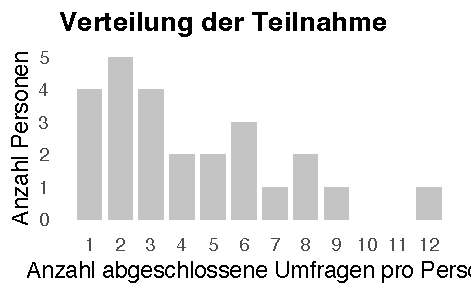
\includegraphics[width=8cm]{Analyse/Plots/survey_counts.pdf}
    \caption{Verteilung der Anzahl abgeschlossener Momentaufnahmen pro Person}
    \label{fig:survey_counts}
\end{figure}

\begin{figure}[h]
    \centering
    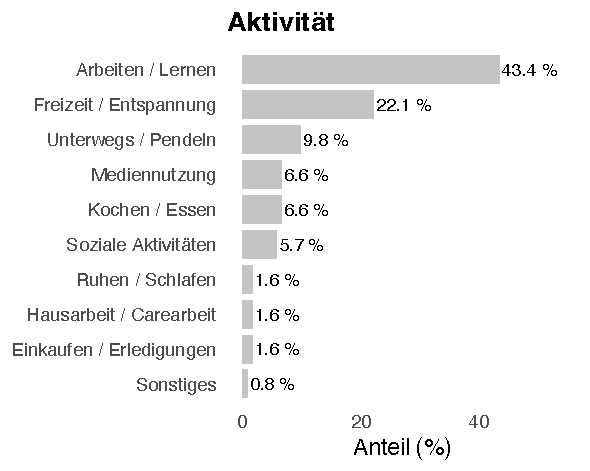
\includegraphics[width=10cm]{Analyse/Plots/cat_dist_activity.pdf}
    \caption{Tätigkeit während der Momentaufnahme}
    \label{fig:survey_activities}
\end{figure}

\begin{figure}[h]
    \centering
    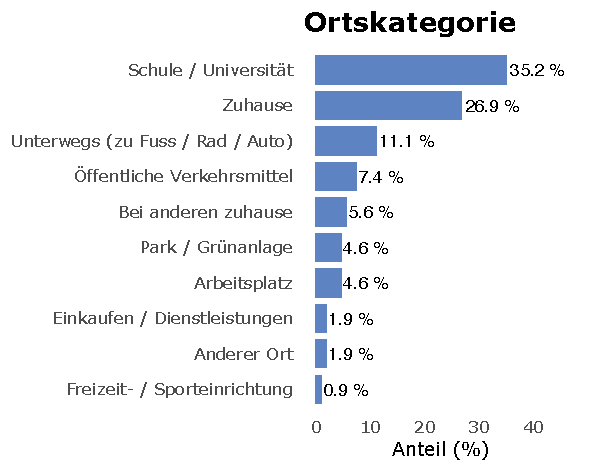
\includegraphics[width=10cm]{Analyse/Plots/cat_dist_location_category.pdf}
    \caption{Aufenthaltsortkategorie während der Momentaufnahme}
    \label{fig:survey_locations}
\end{figure}


\section{Quantitativ-intersektional analysieren -- Ein Widerspruch?}

Wie in \cref{sec:theoretischer_rahmen} dargelegt, besteht eine grundlegende Spannung zwischen den theoretischen Ansprüchen intersektionaler Forschung und den Anforderungen quantitativer Analyseverfahren. Bevor ich die Daten aus der Pilotstudie analysiere, will ich diese Spannung aufgreifen und meinen methodischen Zugang mit \gls{i-maihda} begründen.

Während Intersektionalität auf die komplexe, relationale und kontextabhängige Überlagerung sozialer Kategorien abzielt, verlangen statistische Modelle in der Regel klar definierte, operationalisierte Variablen. Damit einher geht die Gefahr, fluid-dynamische Identitäten in starre Kategorien zu übersetzen und deren soziale Konstruiertheit zu verschleiern \parencite{hancockWhenMultiplicationDoesnt2007, bowlegInvitedReflectionQuantifying2016}. Hinzu kommt, dass viele herkömmliche Verfahren additive oder eindimensionale Effekte modellieren, wodurch genau jene Interdependenzen und Wechselwirkungen nivelliert werden, die intersektionale Ansätze sichtbar machen wollen \parencite{scottIntersectionalityQuantitativeMethods2017}.

Diese methodische Spannung ist nicht nur ein technisches Problem, sondern berührt den Kern intersektionaler Forschung: Die Gefahr, sozial konstruierte Kategorien wie feste, unveränderliche Eigenschaften zu behandeln, steht im Widerspruch zu ihrem theoretischen Verständnis als zeitlich, räumlich und sozial wandelbare Konstrukte. Jede quantitative Operationalisierung muss daher reflexiv mit diesen Grenzen umgehen und das Risiko methodischer Vereinfachungen offenlegen \parencite{rodo-de-zarateDevelopingGeographiesIntersectionality2014, websterCenteringSocialtechnicalRelations2021}.

Vor diesem Hintergrund setze ich in dieser Pilotanalyse \glsxtrfull{i-maihda}\footnotemark ein. \gls{i-maihda} ist ein flexibles, mehrstufiges Analysemodell, das Daten in Gruppen („\glspl{stratum}“) verschachtelt, die sich aus der Kombination mehrerer sozialer Merkmale ergeben. Jede Person gehört genau zu einem solchen sozialen \gls{stratum}. Innerhalb eines sozialen \gls{stratum} können sich die Werte der untersuchten Variablen (\gls[noindex]{zb} (Un-)Wohlbefinden) zwischen Personen unterscheiden, während sich gleichzeitig Unterschiede zwischen den sozialen \glspl{stratum} selbst zeigen.

\footnotetext{Die beiden Begriffe \emph{\glsxtrfull{maihda}} und \emph{\glsxtrfull{i-maihda}} beziehen sich auf dasselbe zugrundeliegende statistische Verfahren; die Bezeichnung mit vorangestelltem \enquote{I} hebt jedoch die intersektionale Perspektive explizit hervor und fordert die Einbettung der Analyse in einen Prozess, der theoretische Entscheidungen und methodische Vereinfachungen laufend kritisch reflektiert \parencite{evansTutorialConductingIntersectional2024}. In dieser Arbeit verwende ich deshalb den Begriff \emph{\gls{i-maihda}}, um diesen Anspruch sichtbar zu machen.}

Aus statistischer Sicht handelt es sich um ein hierarchisches Modell, das mindestens zwei Ebenen umfasst: \textit{Level 1} sind die einzelnen Beobachtungen, \textit{Level 2} die sozialen \glspl{stratum}. \gls{i-maihda} schätzt, wie sich die Gesamtvarianz -- also die Streuung der Messwerte im gesamten Datensatz -- auf unterschiedliche Ebenen verteilt. Dabei wird getrennt zwischen Varianz, die zwischen den sozialen \glspl{stratum} liegt, und Varianz, die innerhalb der sozialen \glspl{stratum} entsteht. Diese Zerlegung erlaubt es zu erkennen, in welchem Ausmass die Kombination sozialer Merkmale systematische Unterschiede im Outcome erklärt und wie viel der Unterschiede auf individuelle oder situative Faktoren zurückzuführen ist. In grossen Datensätzen ermöglicht dieser Ansatz die Modellierung komplexer \glspl{stratum} mit zahlreichen kombinierten Merkmalen.

Der zentrale Vorteil von \gls{i-maihda} gegenüber klassischen Regressionsmodellen liegt darin, dass nicht nur einzelne Haupteffekte und ausgewählte Interaktionsterme berücksichtigt werden, sondern jede Merkmalskombination als eigenständige Analyseeinheit behandelt wird \parencite{scottIntersectionalityQuantitativeMethods2017,bowlegInvitedReflectionQuantifying2016}. Zudem ermöglicht \gls{i-maihda} die Berechnung der sogenannten \enquote{diskriminatorischen Genauigkeit} -- ein Mass dafür, wie trennscharf die gewählten sozialen \glspl{stratum} das Outcome im jeweiligen Kontext erklären \parencite{evansTutorialConductingIntersectional2024}.

\gls{i-maihda} ist aus der epidemiologischen Mehrebenenanalyse hervorgegangen und wurde nicht primär entwickelt, um intersektionale Theorien oder Machtverhältnisse theoretisch zu adressieren. Seine intersektionale Anschlussfähigkeit entsteht erst durch eine bewusste, theoriegeleitete Auswahl der Merkmale, eine reflektierte Modellierung und die Einbettung der Ergebnisse in einen sozialen und politischen Kontext \parencite{grossModellingIntersectionalityQuantitative2023}. In diesem Sinne kann \gls{i-maihda} helfen, die eingangs skizzierte Spannung zwischen theoretischem Anspruch und quantitativer Operationalisierung zu verringern -- sie jedoch nicht vollständig auflösen.

\section{Versuch einer Analyse}

Ziel dieser Pilotanalyse ist es, zu prüfen, ob und in welchem Ausmass sich Unterschiede im situativen Wohlbefinden durch die Kombination mehrerer sozialer \glspl{stratum} und durch situative Kontextfaktoren erklären lassen. Dabei wird ein mehrstufiges Analyseverfahren eingesetzt, das die Messwerte auf verschiedenen Ebenen der Datenhierarchie modelliert. Da die Datengrundlage klein und unbalanciert ist -- viele \glspl{stratum} enthalten nur eine Person und die Zahl der Wiederholungsmessungen pro Person ist gering -- dienen die folgenden Schritte primär der methodischen Illustration und nicht der inhaltlich belastbaren Beantwortung der Forschungsfrage.

Als abhängige Variable wird ein \emph{Wohlbefindensindex} verwendet, der aus fünf Einzelfragen gebildet wurde: \emph{Generelles Wohlbefinden}, \emph{Zufriedenheit}, \emph{Anspannung}, \emph{Energie} und \emph{Zugehörigkeit} (\gls{vgl} \cref{tab:moments}). Alle Items sind auf einen Wertebereich von $0$ bis $1$ skaliert, wobei höhere Werte stets ein positiveres Befinden darstellen. Durch die anschliessende Aggregation mittels des geometrischen Mittels wird vermieden, dass ein sehr hoher Wert in einer Dimension einen niedrigen Wert in einer anderen vollständig ausgleichen kann; zugleich wird der Einfluss einzelner Ausreisser reduziert.

Die zeitinvarianten erklärenden Variablen sind die vier Achsen \emph{\gls[noindex]{gender}}, \emph{Altersgruppe}, \emph{sexuelle Orientierung} und \emph{Äquivalenzeinkommensgruppe} (\gls{vgl} \cref{tab:soziodemografie_gesamt}). Die eindeutige Kombination dieser Merkmale definiert ein soziales \gls{stratum}. Damit gehört jede Person genau zu einem solchen \gls{stratum}.

Die zeitvariablen Kontextmerkmale beziehen sich auf die jeweilige Situation der Momentaufnahme und umfassen Aufenthaltsort (Innen- oder Aussenraum, spezifische Ortskategorie), Anwesenheit und Art der Beziehung zu anderen Personen, Hauptaktivität, Mehrheitsvergleich sowie vier metrische Bewertungen der Umgebung: wahrgenommene Lautstärke, sichtbare Natur, Lebhaftigkeit und empfundene Angenehmheit (\gls{vgl} \cref{tab:moments}).

Zur Modellierung werden kategoriale Variablen als Dummy-Variablen kodiert, wobei jeweils eine Referenzkategorie entfällt, um die statistische Identifizierbarkeit sicherzustellen. Die vier metrischen Umweltbewertungen werden \emph{person-mean}-zentriert, indem von jeder Beobachtung der individuelle Durchschnittswert der jeweiligen Person abgezogen wird. Ein positiver Wert zeigt an, dass eine Situation lauter, naturreicher, lebhafter oder angenehmer erlebt wird als für diese Person gewöhnlich. Dieses Vorgehen trennt kurzfristige Schwankungen innerhalb einer Person von stabilen Unterschieden zwischen Personen.

\subsection*{Modellbildung}

Das erste Modell ($M0_{3L}$) dient dazu, die Gesamtvarianz des Wohlbefindens auf die verschiedenen Ebenen zu zerlegen. Die Ebenen sind:

\begin{enumerate}
    \item \textbf{Level~1:} einzelne Momentaufnahmen,
    \item \textbf{Level~2:} Personen,
    \item \textbf{Level~3:} soziale \glspl{stratum}.
\end{enumerate}

\footnotesize
\begin{longtable}{llll ccc}
    \caption{Übersicht über soziale \glspl[noindex]{stratum}}\label{tab:strata-uebersicht}\\
    \toprule
    Geschl. & Alter & Sex. Orient. & Äquiv.-Eink. & Pers. & Befr. & Befr./Pers.\\
    \midrule
    \endfirsthead
    
    \multicolumn{7}{c}{{Tabelle \thetable{} -- Fortsetzung}} \\
    \toprule
    Geschl. & Alter & Sex. Orient. & Äquiv.-Eink. & Pers. & Befr. & Befr./Pers.\\
    \midrule
    \endhead
    
    \midrule
    \multicolumn{7}{r}{Fortsetzung auf der nächsten Seite}\\
    \endfoot
    
    \bottomrule
    \endlastfoot
    
    weiblich    & 16 -- 25    & heterosexuell & Hoch           & 3 & 13 & 4.33 \\
    männlich    & 16 -- 25    & heterosexuell & Sehr niedrig   & 3 &  9 & 3.00 \\
    männlich    & 16 -- 25    & heterosexuell & \textemdash    & 2 &  9 & 4.50 \\
    weiblich    & 16 -- 25    & heterosexuell & \textemdash    & 2 &  8 & 4.00 \\
    weiblich    & 16 -- 25    & bisexuell     & \textemdash    & 1 & 12 & 12.00\\
    männlich    & 16 -- 25    & heterosexuell & Sehr hoch      & 1 &  9 & 9.00 \\
    männlich    & 16 -- 25    & heterosexuell & Niedrig        & 1 &  8 & 8.00 \\
    männlich    & 16 -- 25    & homosexuell   & Niedrig        & 1 &  7 & 7.00 \\
    weiblich    & 16 -- 25    & heterosexuell & Sehr niedrig   & 1 &  6 & 6.00 \\
    weiblich    & 26 -- 35    & heterosexuell & Sehr niedrig   & 1 &  5 & 5.00 \\
    männlich    & 26 -- 35    & heterosexuell & Sehr hoch      & 1 &  4 & 4.00 \\
    männlich    & 16 -- 25    & homosexuell   & Hoch           & 1 &  3 & 3.00 \\
    männlich    & 16 -- 25    & heterosexuell & Hoch           & 1 &  3 & 3.00 \\
    männlich    & 16 -- 25    & homosexuell   & \textemdash    & 1 &  3 & 3.00 \\
    männlich    & 16 -- 25    & bisexuell     & Sehr niedrig   & 1 &  2 & 2.00 \\
    weiblich    & 16 -- 25    & queer         & Sehr niedrig   & 1 &  2 & 2.00 \\
    \textemdash & \textemdash & \textemdash   & \textemdash    & 1 &  2 & 2.00 \\
    männlich    & 26 -- 35    & bisexuell     & Sehr niedrig   & 1 &  1 & 1.00 \\
    
\end{longtable}
\normalsize


Die Schätzung ergibt, dass rund \SI{8.9}{\percent} der Gesamtvarianz zwischen den \glspl{stratum} liegt, während auf der Personenebene keine eigenständige Varianz feststellbar ist. Mit anderen Worten: Innerhalb desselben \glspl{stratum} unterscheiden sich die mittleren Wohlbefindenswerte der einzelnen Personen in diesen Daten nicht systematisch. Der Grossteil der Varianz ($\approx$\SI{91.1}{\percent}) entfällt auf kurzfristige Schwankungen zwischen verschiedenen Momentaufnahmen derselben Person.

Diese fehlende Varianz auf der Personenebene ist eine direkte Folge der Datenstruktur: Viele \glspl{stratum} bestehen nur aus einer einzelnen Person, und auch bei den übrigen \glspl{stratum} liegt nur eine geringe Zahl an Wiederholungsmessungen pro Person vor. Unter diesen Bedingungen kann das Modell keine stabilen Unterschiede zwischen Personen desselben \gls{stratum} identifizieren. Eine dreistufige Modellierung ist daher hier nicht sinnvoll; die folgenden Schritte basieren auf einer reduzierten zweistufigen Struktur:

\begin{itemize}
    \item \textbf{Level~1:} Momentaufnahmen,
    \item \textbf{Level~2:} \glspl{stratum}.
\end{itemize}

Auch das zweistufige Nullmodell $(M0_{2L})$ ergibt für die sozialen \glspl{stratum} einen \gls{icc} von $\approx$\SI{8.9}{\percent}. Damit lassen sich knapp neun Prozent der Unterschiede im situativen Wohlbefinden auf systematische Differenzen zwischen den sozialen \glspl{stratum} zurückführen.

Im nächsten Schritt $(M1_{2L})$ werden die vier Achsen (\gls[noindex]{gender}, Altersgruppe, sexuelle Orientierung, Äquivalenzeinkommen) als additive Haupteffekte aufgenommen, um den durch Einzeleffekte erklärbaren Anteil dieser Unterschiede zu bestimmen -- ohne Wechselwirkungen zu berücksichtigen. Dieses bewusste \enquote{Auseinanderlegen} verdeutlicht die Spannung zwischen intersektionaler Theorie und quantitativer Analyse: Um den spezifischen Effekt einer Merkmalskombination zu isolieren, werden zunächst die erwarteten Einzeleffekte herausgerechnet. Das verbleibende Mass wird als \emph{intersektionaler Überschuss} bezeichnet.

In diesem Modell sinkt die geschätzte Varianz zwischen den sozialen \glspl{stratum} von \num{0.003024} auf \num{0.001110}, was einer \gls{pev} von rund \SI{63}{\percent} entspricht. Somit lassen sich etwa zwei Drittel der gruppenbezogenen Unterschiede durch die additiven Effekte der vier Achsen erklären; der verbleibende Anteil von rund einem Drittel beruht ausschliesslich auf deren spezifischer Kombination und stellt den intersektionalen Überschuss dar.

Im dritten Modell $(M2_{2L})$ werden zusätzlich die situativen Kontextvariablen aufgenommen. Die geschätzte Varianz zwischen den sozialen \glspl{stratum} sinkt dadurch nahezu auf Null, und auch die verbleibende Restvarianz reduziert sich deutlich. Relativ zum Nullmodell entspricht dies einer erklärten zwischenstratalen Varianz von etwa \SI{99.9}{\percent} sowie einer erklärten Restvarianz von etwa \SI{99.3}{\percent}. Damit lassen sich die Unterschiede im Wohlbefinden zwischen den sozialen \glspl{stratum} in dieser Stichprobe nahezu vollständig durch die Kombination aus Einzelachsen und situativen Kontextfaktoren erklären. Aufgrund der kleinen und unbalancierten Stichprobe ist dieses Ergebnis jedoch mit Vorsicht zu interpretieren.


\subsection*{Analyse variierender Umwelteinflüsse zwischen sozialen Strata}

Die Forschungsfrage dieses Kapitels zielt darauf, zu verstehen, inwieweit sich situative Umweltfaktoren unterschiedlich auf das Wohlbefinden verschiedener sozialer \glspl{stratum} auswirken. Während die bisherigen Modelle lediglich Mittelwertsunterschiede zwischen den \glspl{stratum} abbildeten (\emph{Random Intercepts}), wird dieser Schritt um \emph{Random Slopes} erweitert: Dadurch lässt sich modellieren, ob und wie stark sich die Wirkung einzelner Kontextfaktoren systematisch zwischen den sozialen \glspl{stratum} unterscheidet.

Methodisch eröffnet dieser Ansatz die Möglichkeit, \gls[noindex]{ema}- und \gls[noindex]{gema}-Daten so auszuwerten, dass nicht nur konstante Gruppenunterschiede, sondern auch unterschiedliche Sensitivitäten gegenüber situativen Einflüssen sichtbar werden. In dieser Pilotanalyse dient er der Illustration des methodischen Potenzials; inhaltliche Schlussfolgerungen sind aufgrund der kleinen und unbalancierten Stichprobe nicht möglich.

Für jede der vier metrischen Umweltbewertungen (\emph{Lautstärke}, \emph{sichtbare Natur}, \emph{Lebhaftigkeit} und \emph{empfundende Angenehmheit}) wurde ein separates Mehrebenenmodell mit zufälligen Steigungen geschätzt. Die Umweltvariablen wurden vorab \emph{person-mean}-zentriert und standardisiert, sodass die Koeffizienten als Veränderung des Wohlbefindens pro Anstieg um eine Standardabweichung gegenüber dem individuellen Mittelwert interpretiert werden können. Jedes Modell enthielt die vier sozialen Achsen als feste Effekte, während für die jeweilige Umweltvariable eine variierende Steigung (\emph{Random Slope}) pro \gls{stratum} geschätzt wurde. Aus den Modellen wurden stratum-spezifische Steigungen mit 95\%-Konfidenzintervallen extrahiert und in Tabelle~\ref{tab:effekte-pro-stratum} zusammengeführt.

\footnotesize
\begin{ThreePartTable}
    \begin{TableNotes}[flushleft]
        \item $\Delta$ Wohlbefindensindex pro Anstieg der erklärenden Variable um eine Standardabweichung.
        \item \textbf{Fett} = Effekt ist statistisch signifikant (95\%-Konfidenzintervall schliesst den Wert 0 aus).
        \item (\textemdash = unbekannt)
    \end{TableNotes}
      
    \begin{longtable}{llllr rrrr}
        \caption{Effekte pro Stratum} 
        \label{tab:effekte-pro-stratum} \\
        \toprule
        Geschl. & Alter & Sex. Orient. & Äquiv.-Eink. & Befr. & Lärm & Natur & Lebhaftigkeit & Angenehmkeit \\
        \midrule
        \endfirsthead
        
        \multicolumn{9}{c}{{\bfseries Tabelle \thetable\ -- Fortsetzung}} \\
        \toprule
        Geschl. & Alter & Sex. Orient. & Äquiv.-Eink. & Befr. & Lärm & Natur & Lebhaftigkeit & Angenehmkeit \\
        \midrule
        \endhead
        
        \midrule
        \multicolumn{9}{r}{{Fortsetzung auf der nächsten Seite}} \\
        \endfoot
        
        \bottomrule
        \insertTableNotes
        \endlastfoot
        
        Frau & 16 -- 25 & heterosexuell & hoch         & 13 & \textbf{0.04} & 0.04          & 0.04          & 0.04          \\
        Frau & 16 -- 25 & bisexuell     & ---          & 12 & \textbf{0.04} & 0.05          & \textbf{0.07} & \textbf{0.07} \\
        Mann & 16 -- 25 & heterosexuell & ---          &  9 & \textbf{0.05} & \textbf{0.07} & 0.06          & 0.05          \\
        Mann & 16 -- 25 & heterosexuell & sehr hoch    &  9 & \textbf{0.04} & 0.01          & 0.01          & 0.03          \\
        Mann & 16 -- 25 & heterosexuell & sehr niedrig &  9 & \textbf{0.04} & \textbf{0.07} & 0.03          & 0.03          \\
        Mann & 16 -- 25 & heterosexuell & niedrig      &  8 & \textbf{0.04} & 0.03          & 0.00          & 0.02          \\
        Frau & 16 -- 25 & heterosexuell & ---          &  8 & \textbf{0.04} & 0.02          & 0.04          & 0.03          \\
        Mann & 16 -- 25 & homosexuell   & niedrig      &  7 & \textbf{0.05} & 0.07          & 0.05          & 0.05          \\
        Frau & 16 -- 25 & heterosexuell & sehr niedrig &  6 & \textbf{0.04} & 0.05          & 0.04          & 0.04          \\
        Frau & 26 -- 35 & heterosexuell & sehr niedrig &  5 & \textbf{0.04} & 0.04          & 0.03          & 0.04          \\
        Mann & 26 -- 35 & heterosexuell & sehr hoch    &  4 & \textbf{0.04} & 0.05          & 0.04          & 0.05          \\
        Mann & 16 -- 25 & homosexuell   & hoch         &  3 & \textbf{0.04} & 0.02          & 0.02          & 0.02          \\
        Mann & 16 -- 25 & heterosexuell & hoch         &  3 & \textbf{0.04} & 0.04          & 0.03          & 0.03          \\
        Mann & 16 -- 25 & homosexuell   & ---          &  3 & \textbf{0.04} & \textbf{0.07} & 0.03          & 0.02          \\
        Mann & 16 -- 25 & bisexuell     & sehr niedrig &  2 & \textbf{0.04} & 0.03          & 0.02          & 0.02          \\
        Frau & 16 -- 25 & queer         & sehr niedrig &  2 & \textbf{0.04} & 0.04          & 0.03          & 0.04          \\
    
    \end{longtable}
\end{ThreePartTable}
\normalsize


Einzelne Effektschätzungen waren statistisch signifikant (95\%-Konfidenzintervall schliesst 0 aus). Angesichts der geringen Fallzahlen pro Stratum und der unbalancierten Stichprobe sind diese Resultate jedoch nicht inhaltlich belastbar. Die Auswertung ist hier vor allem als Demonstration zu verstehen, wie heterogene Umwelteffekte entlang sozialer \glspl{stratum} modelliert und dargestellt werden können.

\subsection*{Methodische Beobachtungen und Implikationen}

Die Ergebnisse zeigen, dass sich mit den hier erhobenen \gls[noindex]{ema}- und \gls[noindex]{gema}-Daten grundsätzlich auch stratum-spezifische Umwelteffekte modellieren lassen. Die Umsetzung der \emph{Random-Slopes}-Modelle verlief technisch problemlos; die Modellschätzungen lieferten für jedes \gls{stratum} interpretierbare Effektkoeffizienten und Konfidenzintervalle. 

Gleichzeitig verdeutlicht die Analyse die hohen Anforderungen an die Datengrundlage: Die geringe Fallzahl pro \gls{stratum} führt zu breiten Konfidenzintervallen und erschwert die Trennung systematischer Unterschiede von zufälligen Schwankungen. Die unbalancierte Stichprobenstruktur bewirkt zudem, dass einige Strata vollständig von einzelnen Personen repräsentiert werden, wodurch Schätzungen stark durch individuelle Ausprägungen beeinflusst werden können. 

Die grossen Varianzanteile auf der Ebene der Momentaufnahmen deuten darauf hin, dass kurzfristige, situative Schwankungen einen erheblichen Einfluss auf das Wohlbefinden haben können -- unabhängig von stabilen Gruppenunterschieden. Methodisch unterstreicht dies den Mehrwert von \gls[noindex]{ema}- und \gls[noindex]{gema}-Designs, die solche intraindividuellen Veränderungen erfassen. 

Diese Beobachtungen legen nahe, dass das Verfahren für grössere, stärker ausbalancierte Datensätze geeignet ist, um vergleichbare Forschungsfragen belastbar zu beantworten. In der vorliegenden Pilotstudie dient es vor allem als Machbarkeitsnachweis und zur Identifikation von Herausforderungen, die bei einer weiteren Untersuchung gezielt adressiert werden können.

Darüber hinaus wurde in der Pilotanalyse bewusst darauf verzichtet, die tatsächlichen Standortdaten in die Modellierung einzubeziehen. Angesichts der kleinen Stichprobe hätte dies nur einen geringen inhaltlichen Mehrwert gebracht und potenziell Rückschlüsse auf \gls{bspw} den Wohnort einzelner Teilnehmenden ermöglicht. Sämtliche Standortdaten wurden vor der Veröffentlichung aus dem Datensatz entfernt. Für künftige Erhebungen mit grösserer Fallzahl bietet sich jedoch die Verknüpfung mit hochaufgelösten Kontextinformationen an, beispielsweise mit lokalen Hitzedaten \parencite[siehe][]{burgerModellingSpatialPattern2021} oder präziseren Geofences, um spezifische räumliche Kontexte gezielt zu analysieren.



\clearpage

% LTeX: language=de-CH

\chapter{Diskussion} \label{sec:diskussion}

\section{Potential und Grenzen des entwickelten Erhebungsinstruments}

Die Entwicklung von \textit{InterMind} war im Rahmen dieser Arbeit nicht nur ein technisches, sondern auch ein methodisches Experiment. Ziel war es, mit begrenzten Ressourcen ein Werkzeug zu schaffen, das situative, geolokalisierte Erhebungen zuverlässig durchführen kann -- und dabei die Grundprinzipien von Transparenz, Datenschutz und Anpassungsfähigkeit wahrt. Die im Kapitel skizzierten technischen Entscheidungen waren dabei stets auch methodische Abwägungen: Sie bestimmten nicht nur, wie die App funktioniert, sondern auch, welche Formen der Datenerhebung und -auswertung überhaupt möglich waren.

Besonders prägend war die Wahl eines bewusst reduzierten, clientseitig gesteuerten Systemdesigns. Diese Architektur minimierte Abhängigkeiten von externer Infrastruktur, reduzierte potenzielle Datenschutzrisiken und erlaubte eine transparente, vollständig nachvollziehbare Funktionsweise. Gleichzeitig bedeutete sie den Verzicht auf Funktionen, wie sie in komplexeren GEMA-Implementierungen üblich sind -- etwa geofence-basierte Trigger oder serverseitige Kontextlogiken. Dadurch blieb die App methodisch auf feste, vordefinierte Erhebungszeitpunkte beschränkt und konnte nicht adaptiv auf räumliche oder kontextuelle Veränderungen reagieren. Für explorative Pilotstudien wie die vorliegende war dies ausreichend, in längerfristigen oder gross angelegten Projekten wäre jedoch eine dynamischere, kontextsensitivere Architektur wünschenswert.

Die Entscheidung zur Open-Source-Veröffentlichung stellt einen zentralen Bestandteil des Projekts dar. Sie ermöglicht anderen Forschenden nicht nur die Nachnutzung des Codes, sondern schafft auch die Grundlage für kollaborative Weiterentwicklungen. Gleichzeitig machte die Erfahrung mit den App-Store-Gatekeeping-Prozessen deutlich, dass Offenheit allein keine Garantie für breite Zugänglichkeit ist: Die Distribution über zentrale Plattformen bleibt an kommerzielle und intransparente Strukturen gebunden, die auch nicht-kommerzielle, wissenschaftliche Projekte einschränken können. Hier zeigt sich ein strukturelles Spannungsfeld zwischen der offenen, gemeinschaftsorientierten Logik von Open-Source-Software und den geschlossenen, marktkontrollierten Ökosystemen der grossen Plattformanbieter.

Im Rückblick wird deutlich, dass die App-Entwicklung in dieser Form einerseits ein funktionierendes, forschungsnahes Werkzeug hervorgebracht hat, andererseits aber auch klare Grenzen aufweist. Diese liegen weniger in der Stabilität oder Bedienbarkeit, sondern vielmehr in der eingeschränkten Kontextanpassung, der fehlenden Echtzeitauswertung und der aufwändigen Anpassbarkeit für andere Forschungssettings. Zukünftige Iterationen könnten hier ansetzen -- etwa durch die Ergänzung serverseitiger Module, die Entwicklung eines webbasierten Dashboards für Monitoring und Feedback, oder die modularisierte Integration zusätzlicher Erhebungsmethoden.

Damit verdeutlicht \textit{InterMind} sowohl die Chancen als auch die Grenzen einer eigenständigen Entwicklung im Rahmen einer Abschlussarbeit: Sie eröffnet Handlungsspielräume, schafft technologische Unabhängigkeit im Entwicklungsprozess und macht Forschungsinfrastruktur transparent -- bleibt aber eingebettet in grössere, teils restriktive Strukturen, die den Handlungsspielraum letztlich mitbestimmen.

\section{Reflexion und Weiterentwicklungspotenzial des Fragebogens}

Der entwickelte Fragebogen erwies sich im Feld als grundsätzlich funktional und gut in den Ablauf der Studie integrierbar. Er erfüllte die Anforderung, situative Erhebungen in kurzer Zeit und mit geringer Belastung für die Teilnehmenden durchführen zu können. Gleichzeitig zeigte sich jedoch, dass diese Stärken teilweise mit methodischen Einbussen erkauft wurden, die den wissenschaftlichen Anspruch der Erhebung begrenzen.

Besonders deutlich wird dies bei der Auswahl der Items zur Erfassung situativen affektiven Wohlbefindens. Die gewählten Dimensionen -- darunter „generelles Wohlbefinden“, Zufriedenheit, Anspannung, Energie und Zugehörigkeit -- erlaubten zwar eine kompakte Erfassung, entstanden jedoch nicht aus einer stringenten theoretischen Modellierung heraus. Diese pragmatische Herangehensweise erleichterte zwar die Umsetzung im Rahmen einer Mehrfacherhebung, führte aber zu einer geringeren konzeptuellen Schärfe und erschwerte den direkten Vergleich mit bestehenden Studien.

Auch der Verzicht auf etablierte standardisierte Skalen hatte ambivalente Folgen. Er trug dazu bei, den Fragebogen schlank zu halten und die Akzeptanz bei den Teilnehmenden zu erhöhen, schränkte jedoch die Vergleichbarkeit der Daten und ihre Anschlussfähigkeit an bestehende Forschungsinstrumente ein. Eine gekürzte, modulare Integration validierter Skalen hätte hier einen Ausgleich zwischen Praktikabilität und methodischer Robustheit schaffen können.

Die mehrsprachige Umsetzung des Instruments war ein wichtiger Schritt in Richtung Zugänglichkeit, blieb jedoch ohne formalisierte Validierung durch muttersprachliche Expert:innen. Dadurch ist nicht auszuschliessen, dass inhaltliche Nuancen, insbesondere bei affektiven Zustandsbeschreibungen, zwischen den Sprachversionen leicht variierten. Diese Unsicherheiten verstärkten sich bei sensiblen Konzepten wie \gls[noindex]{race}, für das im deutschsprachigen Kontext keine etablierten, diskriminierungssensiblen Kategorien verfügbar sind. Die gewählte Operationalisierung über Geburts- und Aufenthaltsland senkte zwar die Erhebungsbarrieren, konnte die Komplexität rassifizierter Erfahrungen jedoch nur unvollständig erfassen.

Schliesslich war der Entwicklungsprozess des Fragebogens zwar iterativ angelegt und von kontinuierlichem Feedback begleitet, basierte jedoch nicht auf einem formalen Pretest mit einer breiten und divers zusammengesetzten Testgruppe. Dadurch wurden potenzielle Verständnisschwierigkeiten oder kulturelle Unschärfen nur in begrenztem Umfang sichtbar.

Insgesamt bleibt festzuhalten, dass der Fragebogen in seiner vorliegenden Form eine praktikable, aber methodisch eingeschränkte Lösung darstellt. Für zukünftige Studien bieten sich mehrere Ansatzpunkte zur Weiterentwicklung: eine engere theoretische Anbindung der Items, die gezielte Integration gekürzter validierter Skalen, ein systematischeres Übersetzungs- und Validierungsverfahren sowie umfassendere Pretests. Auf diese Weise liesse sich die inhaltliche Aussagekraft der Erhebung stärken, ohne die für hochfrequente Befragungen notwendige Niedrigschwelligkeit aufzugeben.

\section{Gedanken für weiterführende Forschung}

% \subsection{Verbesserungsvorschläge zur Erhöhung der Teilnahmequote}

% \subsection{Optimierung der intersektionalen Datenerhebung und Analyse}

% \subsection{Integration qualitativer Verfahren}

% Standorterhebung nicht verwendet. damit eigentlich ema und nicht gema gemacht. da ich das alles auch nicht noch verknüpft habe mit weiteren indikatoren wie bspw temperatur oder so.


% ohne technische details mal hier rüberkopiert:

% \section{Eigenständig, aber nicht unabhängig -- Entwicklung im Plattformzeitalter}

% Die Entwicklung von \gls{intermind} war mein erstes grösseres Projekt in \gls{typescript} und mit \gls{reactnative}. Die Umstellung vom strikt objektorientierten Denken in \gls{java} auf den dynamischeren, komponentenbasierten Ansatz war anspruchsvoll, aber enorm lehrreich. Insbesondere das konsequente Anwenden der \gls{solid}-Prinzipien half dabei, die Struktur der Anwendung nachvollziehbar zu halten -- gerade in einem neuen Ökosystem. Die App funktioniert stabil, sieht gut aus, und hat ihren Zweck erfüllt.

% Trotz einer bewussten Orientierung an Prinzipien wie \gls{solid} und einem grundlegenden Architekturkonzept zeigte sich im Verlauf der Entwicklung, dass eine noch systematischere Auseinandersetzung mit der Softwarearchitektur hilfreich gewesen wäre. Zwar wurde auf eine modulare Struktur geachtet, viele Designentscheidungen wurden jedoch eher situativ getroffen und nicht im Sinne eines übergeordneten Gesamtdesigns immer wieder überprüft. Gerade im weiteren Projektverlauf wäre es sinnvoll gewesen, gezielt zu früheren architektonischen Überlegungen zurückzukehren und diese zu reflektieren oder anzupassen.

% Methoden wie \emph{Test-Driven Development} hätten diesen Prozess zusätzlich stützen können, indem sie klare Schnittstellen und Verantwortlichkeiten frühzeitig erzwingen. Auch der Aufbau automatisierter Tests und eine kontinuierlich integrierte Codeanalyse hätten dazu beigetragen, Fehlerquellen frühzeitig zu identifizieren und die langfristige Wartbarkeit der Anwendung zu verbessern. Viele kleinere Schwächen im Code wurden zwar pragmatisch behoben, ein strukturierteres Qualitätsmanagement hätte jedoch die Notwendigkeit späterer Refactoring-Prozesse deutlich reduziert.

% In diesem Sinne reiht sich die App auch in eine typische Dynamik vieler \gls{opensource}-Projekte ein: Sie wurde aus einem konkreten Forschungsbedarf heraus entwickelt, funktioniert zuverlässig, ist öffentlich dokumentiert -- aber nicht in jedem Teilbereich optimal strukturiert. Durch die Offenlegung des Quellcodes besteht jedoch die Möglichkeit, dass andere Entwickler\genderstern innen auf dieser Grundlage aufbauen, Verbesserungsvorschläge einbringen oder eigene Erweiterungen umsetzen.

% \vspace{1em}

% Trotz stabiler Funktionalität und durchdachter Grundstruktur weist das entwickelte System klare Begrenzungen auf -- insbesondere im Hinblick auf die situative Reaktionsfähigkeit und Kontextanpassung. So verzichtet \gls{intermind} bewusst auf kontinuierliches Geotracking, automatisierte Trigger oder serverseitige Kontextlogiken, wie sie in anderen \glsxtrshort{gema}-Systemen Anwendung finden.

% Ein Beispiel dafür bietet das im Rahmen einer kanadischen Studie zu Nationalparks entwickelte \glsxtrshort{health}-Plattform \parencite{wrayHealthyEnvironmentsActive2025}. Die Dokumentation zu diesem Tool ist erst während der Entstehung dieser Arbeit als Preprint veröffentlicht worden. Die App wird derzeit exklusiv im Rahmen des \textit{ParkSeek}-Projekts\footnote{\href{https://parkseek.ca/}{parkseek.ca}} eingesetzt und ist nicht öffentlich zugänglich. Ihre zugrundeliegende Systemarchitektur erlaubt eine kontinuierliche Standorterfassung und serverseitige Kontextverarbeitung, wodurch komplexe Logiken wie geofence-basierte Trigger umgesetzt werden können. So lassen sich etwa Benachrichtigungen auslösen, wenn sich Teilnehmende über längere Zeit in spezifischen Umwelten aufhalten. Diese technisch anspruchsvolle Lösung erlaubt eine besonders enge Verzahnung zwischen räumlichem Verhalten und situativer Befragung, geht jedoch mit einem hohen Aufwand sowie erheblichen Anforderungen an Datenschutz, Datenmanagement und Infrastruktur einher.

% Im Rahmen eines Bachelorprojekts wäre die Implementierung eines derart umfassenden Systems weder zeitlich noch organisatorisch realistisch gewesen. Stattdessen wurde ein datensparsamer, clientseitig gesteuerter Ansatz gewählt, der mit begrenzten Mitteln eine funktionale, transparente und reflektierte Umsetzung ermöglicht. Die Entscheidung für ein reduziertes Systemdesign war damit nicht nur eine Frage des Aufwands, sondern auch ein bewusster Kompromiss zugunsten von Kontrollierbarkeit und Datenschutz.

% Eine weitere Limitation des aktuellen Systemdesigns liegt im Fehlen eines serverseitigen Dashboards oder einer integrierten Auswertungsoberfläche. Es besteht keine Möglichkeit, Rückmeldungen in Echtzeit zu visualisieren, aggregierte Antworten einzusehen oder Monitoring-Funktionen während der Erhebung zu nutzen. Solche Features wären insbesondere für die Steuerung längerer Erhebungsphasen, die Qualitätssicherung oder für Feedbackschleifen mit den Teilnehmenden von Vorteil gewesen. Ihre Umsetzung hätte jedoch zusätzliche Entwicklungsressourcen sowie eine komplexere Backend-Architektur vorausgesetzt. Gleichwohl bleibt die Möglichkeit bestehen, entsprechende Funktionen in zukünftigen Iterationen oder auf Basis der veröffentlichten Codebasis nachzurüsten.

% \vspace{1em}

% Die Erfahrungen rund um die Veröffentlichung in den App Stores hat zentrale Spannungsfelder digitaler Infrastruktur deutlich gemacht. Obwohl die App funktional einsatzbereit war und über TestFlight bzw. den Play Store zugänglich gemacht werden konnte, blieb die reguläre Veröffentlichung im Apple App Store aufgrund einer intransparenten Ablehnung verwehrt.

% Solche Prozesse offenbaren strukturelle Abhängigkeiten, die weit über dieses Projekt hinausgehen: Zwei gigantische multinationale Tech-Konzerne kontrollieren in weiten Teilen den Zugang zu digitaler Infrastruktur. Dabei wirken sie zugleich als Regelsetzer, Infrastrukturbetreiber und ökonomische Gatekeeper. Diese doppelte Rolle ist nicht demokratisch legitimiert, aber mit erheblicher Lenkungsmacht verbunden. Gerade nicht-kommerzielle, experimentelle oder aktivistische Projekte sind von diesen Kontrollmechanismen besonders betroffen, da sie sich nicht ohne Weiteres den geforderten Verwertungslogiken oder Standardprozessen unterwerfen.

% Auch wenn Open-Source-Prinzipien allein diese strukturellen Hürden nicht auflösen können, war die Entscheidung zur Veröffentlichung des Quellcodes dennoch zentral: Sie schafft Transparenz, ermöglicht Weiterentwicklung und signalisiert ein bewusstes Gegenmodell zu proprietären, intransparenten Systemen. Gleichzeitig offenbart sich hier ein grundlegendes Spannungsfeld: Die offene, zugängliche und gemeinschaftsorientierte Logik von \gls{opensource}-Software steht in einem scharfen Kontrast zu den geschlossenen, marktkontrollierten Strukturen kommerzieller Distributionsplattformen. Wer eine App entwickeln und öffentlich zugänglich machen will, ist faktisch gezwungen, sich diesen Plattformen zu unterwerfen.

% Die Arbeit an der App war dabei nicht nur funktional motiviert, sondern auch von der Erfahrung getragen, ein eigenes digitales Werkzeug gestalten zu können -- mit all seinen Herausforderungen, aber auch mit dem unmittelbaren Lernerfolg und der Freude am konkreten Entstehungsprozess. Gerade vor dem Hintergrund einer zunehmend von privatwirtschaftlichen Plattformen dominierten digitalen Infrastruktur bleibt die Fähigkeit, eigene Werkzeuge zu entwickeln, ein wichtiger Akt technischer Aneignung.

% auch hier nicht nochmal entwickelnd erklären, je nachdem acuh ganz sein lassen

% \section{Klar, verständlich, iterativ -- Der Weg zum finalen Fragebogen}

% Die sprachliche Gestaltung der Fragebogen-Items stellte im Entwicklungsprozess eine zentrale methodische Herausforderung dar. Ziel war es, die Befragung möglichst zugänglich, verständlich und gleichzeitig inhaltlich präzise zu gestalten. Da die Befragung explizit auf eine intersektionale Analyse abzielt, wurde besonderer Wert darauf gelegt, die sprachliche Zugänglichkeit möglichst breit zu gewährleisten. Folglich wurde der Fragebogen bewusst mehrsprachig konzipiert und auf Deutsch, Englisch sowie Französisch umgesetzt. Weitere Sprachversionen wären zwar aus Sicht der intersektionalen Zugänglichkeit wünschenswert gewesen, scheiterten jedoch am hohen Aufwand für qualitativ hochwertige und inhaltlich konsistente Übersetzungen.

% Ein grundsätzliches Anliegen war eine möglichst direkte, adressierende Sprache in der \enquote{Du}-Form, um einen niederschwelligen Zugang zur Befragung zu fördern und hierarchische Distanz zwischen Forschenden und Teilnehmenden zu reduzieren. Gleichzeitig mussten die Formulierungen prägnant, alltagsnah und schnell erfassbar sein, da insbesondere die situativen Erhebungen kurz gehalten werden sollten. Hier ergab sich ein methodischer Balanceakt: Einerseits sollte die Befragung leicht verständlich bleiben, andererseits mussten komplexe Konzepte in zugänglicher Sprache operationalisiert werden. So wurde \gls{bspw} das Konzept der \gls{intersektionalitaet} im Einführungsteil des Fragebogens erläutert, danach jedoch bewusst vermieden, um unnötige Barrieren zu reduzieren. Stattdessen wurden alternative Formulierungen wie \enquote{persönliche Merkmale} verwendet, die jedoch teilweise inhaltliche Unschärfen mit sich brachten. 

% Besonders deutlich wurde diese Herausforderung im Umgang mit dem Konzept \gls[noindex]{race}. Gerade im deutschsprachigen Kontext existieren hier nur schwer geeignete Begrifflichkeiten: Formulierungen wie \enquote{Rasse} oder \enquote{Ethnizität} sind entweder sprachlich ungebräuchlich, problematisch oder stark mit kolonialen und biologistischen Zuschreibungen assoziiert \parencite[\gls{vgl}][]{roigIntersectionalityEuropeDepoliticized2018}. Alternativ verwendete Begriffe wie \enquote{Herkunft} oder \enquote{Aussehen} sind wiederum unpräzise und greifen die Dimension rassifizierter Diskriminierung nur unvollständig auf.

% Die Übersetzung der Items erfolgte nicht wörtlich, sondern sinngemäss, wobei insbesondere bei affektiven Zustandsbeschreibungen semantische Abstimmungen zwischen den Sprachversionen vorgenommen wurden. Dabei wurden auch kulturelle Unterschiede in der Alltagsverwendung bestimmter Begriffe berücksichtigt. Dieser Kompromiss ermöglichte trotz beschränkter Ressourcen eine hinreichend konsistente Mehrsprachigkeit, brachte jedoch gewisse methodische Limitierungen hinsichtlich der Vergleichbarkeit der Sprachversionen mit sich.

% Der beschriebene Sprach- und Übersetzungsprozess war eingebettet in einen breiteren, iterativen Entwicklungsprozess, der sowohl auf der Analyse bestehender Literatur als auch auf kontinuierlichem Feedback basierte. Ausgangspunkt bildeten Studien wie die Urban-Mind-Studie \parencite{bakolisUrbanMindUsing2018}, deren methodische Ansätze zur Erhebung situativen Wohlbefindens und räumlicher Wahrnehmung als Orientierung dienten. Diese Ansätze wurden jedoch um eigene Überlegungen zur intersektionalen Erhebung sozialer Positionierung ergänzt und in mehreren Durchläufen kritisch reflektiert.

% Während der Testphase der App Entwicklung (Siehe \cref{sec:app_entwicklung_feldtest}) sind ebenfalls zahlreiche kleinere Rückmeldungen zu Formulierungen und sprachlichen Feinheiten eingegangen. Diese wurden laufend eingearbeitet. Ebenfalls wurde der Fragebogen mit der betreuenden Dozentin durchgegangen und danach ebenfalls nochmals entsprechend überarbeitet.
% Ein wiederkehrendes methodisches Kriterium bei diesen Diskussionen war stets, die Belastung für Teilnehmende so gering wie möglich zu halten, ohne zentrale Aspekte der Forschungsfrage zu vernachlässigen. Durch den iterativen Ansatz konnte die Perspektive potenzieller Befragter frühzeitig einbezogen werden, was zu einer praxisnahen Optimierung der Items und des Fragebogenaufbaus führte.

% Im Rückblick lassen sich einige Punkte identifizieren, die bei einer erneuten Durchführung anders gestaltet werden könnten. Die Auswahl der Wohlbefindensdimensionen erfolgte nicht vollständig theoriegeleitet; insbesondere das Item „generelles Wohlbefinden“ wirkt im Nachhinein wenig trennscharf. Eine stärkere konzeptuelle Fundierung der Items wäre sinnvoll, um die Aussagekraft einzelner Skalen zu erhöhen.

% Der Verzicht auf standardisierte Skalen ermöglichte eine kompakte Erhebung, schränkt jedoch Vergleichbarkeit und Validität ein. Eine modularisierte Integration validierter Instrumente -- etwa in gekürzter Form -- könnte eine tragfähige Alternative darstellen.

% Die mehrsprachige Umsetzung war aus methodischer Sicht wichtig, konnte jedoch mangels Ressourcen nicht vollständig abgesichert werden. Eine zusätzliche Validierung durch muttersprachliche Expert:innen wäre wünschenswert gewesen, um semantische Konsistenz über Sprachversionen hinweg besser zu gewährleisten.

% Insgesamt zeigen sich an mehreren Stellen Stellschrauben für eine künftige Weiterentwicklung -- etwa durch eine engere theoretische Anbindung, gezielte Pretests oder eine systematischere Überprüfung von Übersetzungen und Antwortformaten. Gleichzeitig hat sich der gewählte Zugang als praktikabel und kontextsensibel erwiesen, insbesondere im Hinblick auf Zugänglichkeit und situative Anschlussfähigkeit.

% Besonders herausfordernd war die Erfassung von \gls[noindex]{race}. Im europäischen Kontext existieren kaum etablierte Kategorien, die rassifizierte Zugehörigkeiten erfassen, ohne problematische koloniale oder biologistische Zuschreibungen zu reproduzieren \parencite[\gls{vgl}][]{roigIntersectionalityEuropeDepoliticized2018}. Anders als in der US-amerikanischen Tradition, in der standardisierte Selbstkategorisierungen weit verbreitet sind, fehlen im hiesigen Kontext praktikable, breit akzeptierte Formate für quantitative Erhebungen. 

% Vor diesem Hintergrund wurde aus pragmatischen Gründen lediglich erfasst, ob Teilnehmende aktuell in einem anderen Land leben als in jenem, in dem sie geboren wurden. Diese Lösung reduzierte die Erhebungsbarrieren, blieb jedoch analytisch begrenzt: Sie kann nur indirekt auf rassifizierte Erfahrungen hinweisen und wird der Komplexität intersektionaler Ungleichheiten nicht gerecht. Rückblickend wäre eine offene, selbstbezeichnungsbasierte Erhebung vorzuziehen gewesen, um dieser sozialen Dimension angemessen Sichtbarkeit zu verleihen.

% Vor diesem Hintergrund wurde ein eigener, stark reduzierter Item-Satz entwickelt, um zentrale Dimensionen des Wohlbefindens situativ abbilden zu können. Ausgewählt wurden fünf Dimensionen: generelles Wohlbefinden, Zufriedenheit, Anspannung, Energie und Zugehörigkeit. Die Antworten wurden über lineare Slider-Skalen erfasst, um eine schnelle und intuitive Bearbeitung zu ermöglichen. 

% Diese Lösung stellt jedoch einen methodischen Kompromiss dar. Die Auswahl der Dimensionen erfolgte nicht auf Basis eines validierten theoretischen Modells, sondern primär pragmatisch und unter der Prämisse minimaler Befragungsdauer. Entsprechend ist die Validität und Vergleichbarkeit der erhobenen Werte eingeschränkt. Rückblickend erweist sich dies als Schwachpunkt der Studie: Die Messung bleibt inhaltlich und konzeptuell weniger trennscharf als wünschenswert, und es fehlt an einer etablierten Referenz, um die Ergebnisse eindeutig einzuordnen. Eine künftige Weiterentwicklung sollte daher auf einer systematischeren Konzeptualisierung beruhen und -- sofern möglich -- gekürzte, validierte Instrumente integrieren, die auf die Anforderungen situativer Mehrfacherhebungen angepasst sind.

Future forschung:
RQ-M4 (Kontextintegration ohne „Big GPS“): Wie lassen sich situative Kontextvariablen der Umgebung sinnvoll integrieren, wenn Standortdaten bewusst sparsam genutzt werden (z. B. punktuelle Location, selbstberichtete Kontexte), ohne die intersektionale Logik zu verwässern?


Wenn ich code veröffentliche expose ich mich auch. open source hat also auch seine nachteile. es bracuht mut und ein verständnis dass es auf jeden fall nicht perfekt ist. gerade als nicht informatiker finde ich das schon sehr schwer.

soll ich irgendwo noch meine eigene position reflektieren? finde ich hier irgendwie nicht so wichtig wie wenn ich etwas auswerten würde. was haben meine erfahrungen und meine soziale position damit zu tun wie ich code? das ist halt einigermassen politisch, andere hätten jetzt versucht daraus ein business zu machen. motivation zu code ist halt wirklich aus einer politischen überzeugung heraus entstanden. klar, auch wissenschaftlich argumentiert aber der willen war vor der theorie da.

\begin{quote}
    \emph{Wie lässt sich der Einfluss räumlicher Umgebungen auf das affektive Wohlbefinden intersektional positionierter Personen erfassen und analysieren?}
\end{quote}

\begin{enumerate}
    \item Wie gestalte ich einen Erhebungsansatz, der affektives Wohlbefinden intersektional positionierter Personen gemeinsam mit relevanten Kontextmerkmalen wiederholt \textit{in situ} erfasst?
    \item Welche Anforderungen ergeben sich aus einer kritisch-digitalen Perspektive an ein Werkzeug, das solche Erhebungen ermöglicht, und wie realisiere ich diese Anforderungen in einer konkreten Umsetzung?
    \item Wie geeignet sind die in einer Pilotstudie erhobenen Daten für eine intersektionale Mehrebenenmodellierung?
\end{enumerate}


daten aus der pilotstudie lassen eigentlich nur sehr bedingt eine qualitative beantwortung der dritten frage zu. sehr wenig daten aus einer sehr homogenen gruppe.

% ernsthafte frage: Wie kann es sein, dass in zeiten von open science und open data die wissenschaft es offentichtlich nicht schafft keine open source tools zu entwickeln? Fehlt da irgendwie die affinität? Spielen kommerzielle gedanken eine rolle der entwickelnden unternehmen oder was steckt dahinter?

\clearpage


% ------------------ Glossar
%TC:ignore
\clearpage
\addcontentsline{toc}{chapter}{Glossar}
\printglossary[label=sec:glossary]



% ----------------- Bibliographie ------------------
\clearpage
\phantomsection
\printbibliography[heading=bibintoc, title=Literaturverzeichnis]

\clearpage

\phantomsection
\section*{Hinweis für den Einsatz von künstlicher Intelligenz}

Dieses Arbeit wurde punktuell mit KI-basierten Tools überarbeitet. Zur sprachlichen Optimierung kamen DeepL Write und LanguageTool zum Einsatz, während ChatGPT von OpenAI genutzt wurde, um Feedback zur Verständlichkeit und Struktur der Arbeit zu erhalten. Im Rahmen des Coding-Prozesses wurden zudem ChatGPT (OpenAI) und Claude (Anthropic) unterstützend verwendet. Es wurde jedoch keine KI zur Erstellung von Originalinhalten eingesetzt.


\clearpage

\phantomsection
\section*{Selbstständigkeitserklärung}

Ich erkläre hiermit, dass ich diese Arbeit selbstständig verfasst und keine anderen als die angegebenen Quellen benutzt habe. Alle Stellen, die wörtlich oder sinngemäss aus Quellen entnommen wurden, habe ich als solche gekennzeichnet. Mir ist bekannt, dass andernfalls der Senat gemäss Artikel 36 Absatz 1 Buchstabe r des Gesetzes vom 5. September 1996 über die Universität zum Entzug des aufgrund dieser Arbeit verliehenen Titels berechtigt ist.

Für die Zwecke der Begutachtung und der Überprüfung der Einhaltung der Selbständigkeitserklärung bzw. der Reglemente betreffend Plagiate erteile ich der Universität Bern das Recht, die dazu erforderlichen Personendaten zu bearbeiten und Nutzungshandlungen vorzunehmen, insbesondere die schriftliche Arbeit zu vervielfältigen und dauerhaft in einer Datenbank zu speichern sowie diese zur Überprüfung von Arbeiten Dritter zu verwenden oder hierzu zur Verfügung zu stellen.

\vspace{8cm}

\noindent Bern, \today

\vspace{2cm}

\noindent\rule{6cm}{0.4pt} \\
\noindent Lukas Batschelet




\clearpage
\pagenumbering{alph}
   
   \phantomsection
\appendix
\addcontentsline{toc}{chapter}{Anhang}



\begin{appendices}

\bookmarksetup{startatroot=false}   % Alle folgenden Überschriften ↓ im pdf eine Ebene tiefer

\addtocontents{toc}{\protect\setcounter{tocdepth}{-1}}



\chapter{Fragebogen}
\label{app:appendix_fragebogen}

Deutsche Version des Fragebogens. Die übersetzten Versionen auf Englisch und Französisch können im \gls[noindex]{github}-Repository\footnote{\href{https://raw.githubusercontent.com/lbatschelet/Designing-InterMind/main/Questionnaire.xlsx}{https://raw.githubusercontent.com/lbatschelet/Designing-InterMind/main/Questionnaire.xlsx}} der Arbeit heruntergeladen werden.


\section*{Hallo!}
Schön bist Du hier!

In dieser App wirst Du eine Woche lang drei Mal am Tag kurze Fragen zu Deinem aktuellen Wohlbefinden und zu Deiner Umgebung beantworten.

Deine Antworten helfen uns dabei, besser zu verstehen, wie Menschen verschiedene Orte erleben – und wie diese Erfahrungen mit unterschiedlichen Lebenssituationen zusammenhängen.

\hrulefill

\section*{Worum geht es in dieser Studie?}
Wie wir uns an einem Ort fühlen, hängt stark von unserer Umgebung ab. Manche Orte wirken beruhigend, vertraut oder einladend. Andere lassen uns unruhig werden, ausgegrenzt erscheinen oder fehl am Platz fühlen.

Solche Erfahrungen sind jedoch nicht für alle Menschen gleich. Sie können davon abhängen, wie wir an einem Ort wahrgenommen und behandelt werden – z.\,B. aufgrund von Geschlecht, Herkunft, Sprache, Aussehen oder anderen Merkmalen, die unsere gesellschaftliche Position prägen.

\subsection*{Was meinen wir mit Wohlbefinden?}
Wohlbefinden kann vieles bedeuten. Manchmal geht es dabei um etwas Langfristiges – etwa, wie zufrieden wir mit unserem Leben insgesamt sind, wie gesund wir uns fühlen oder ob wir uns sicher und unterstützt fühlen.

In dieser Studie interessiert uns jedoch vor allem das \textbf{momentane Wohlbefinden}: Wie geht es Dir \emph{jetzt gerade}, an diesem Ort, in dieser Situation?  
Wohlbefinden umfasst sowohl \textbf{körperliche} Aspekte (z.\,B. Müdigkeit, Wärme, Ruhe) als auch \textbf{psychische} Empfindungen (z.\,B. Zufriedenheit, Sicherheit, Zugehörigkeit).

\subsection*{Wer führt die Studie durch?}
Diese Bachelorarbeit wird am Geographischen Institut der Universität Bern von Lukas Batschelet durchgeführt und von Prof.\ Dr.\ Carolin Schurr sowie Dr.\ Moritz Gubler betreut.

\subsection*{Was ist das Ziel dieser Studie?}
Wir untersuchen, wie sich verschiedene Merkmale – einzeln oder kombiniert – auf das momentane Wohlbefinden auswirken.

\subsection*{Wie läuft die Teilnahme ab?}
Die Studie dauert eine Woche; in dieser Zeit erhältst Du dreimal täglich eine Kurzbefragung auf Deinem Smartphone:

\begin{itemize}\setlength{\itemsep}{0pt}
  \item Ort, an dem Du Dich befindest
  \item Deine Tätigkeit dort
  \item Dein aktuelles Befinden
  \item Gefühl der Zugehörigkeit oder Fremdheit
\end{itemize}

Jede Befragung ist eine Stunde lang verfügbar; verpasste Befragungen kannst Du einfach überspringen.

\hrulefill

\section*{Einwilligung zur Teilnahme}
Bevor Du mit der Befragung startest, bitten wir Dich um Deine Zustimmung zur Teilnahme.  
Die Teilnahme ist freiwillig; einzelne Fragen können übersprungen und die Teilnahme jederzeit beendet werden. In den App-Einstellungen kannst Du Deine Daten nachträglich vollständig löschen.

\subsection*{Welche Daten werden erhoben?}
\begin{itemize}\setlength{\itemsep}{0pt}
  \item Angaben zu Deiner Person (z.\,B. Alter, Geschlecht, Bildung)
  \item Antworten zu Deinem aktuellen Befinden und Aufenthaltsort
  \item Standortdaten (sofern freigegeben)
\end{itemize}

\subsection*{Wie gehen wir mit Deinen Daten um?}
\begin{itemize}\setlength{\itemsep}{0pt}
  \item Keine Speicherung von Namen, E-Mail-Adressen o.\,ä.
  \item Anonymisierte Speicherung auf einem gesicherten Server in der Schweiz
  \item Keine Bewegungsprofile oder dauerhafte Standortverläufe
  \item Nutzung ausschliesslich für wissenschaftliche Zwecke, keine Weitergabe an Dritte
\end{itemize}

Mit \enquote{Ich stimme zu} bestätigst Du, dass Du die Informationen verstanden hast und freiwillig teilnimmst. Weitere Details findest Du in unserer \href{https://intermind.ch/privacy-policy.html}{Datenschutzrichtlinie}.

\hrulefill

\section*{Benachrichtigungen}
Damit Du keine Befragung verpasst, senden wir Dir Benachrichtigungen, sobald ein neues Umfrageslot startet (jeweils eine Stunde Antwortzeit).  
Du kannst die Benachrichtigungen in den Geräteeinstellungen abschalten – dann besteht jedoch die Gefahr, Befragungen zu verpassen.  
Wir empfehlen, sie eingeschaltet zu lassen, um möglichst viele unterschiedliche Situationen zu erfassen.

\hrulefill

\section*{Standort}
Um räumliche Muster zu erkennen, bitten wir Dich, die Standortfreigabe zu erlauben. So können wir z.\,B. unterscheiden, ob Erleben an belebten Plätzen anders ist als in ruhigen Gegenden – ohne Deinen Namen oder exakte Adressen zu kennen.

Standortdaten werden ausschliesslich anonymisiert gespeichert und nicht dauerhaft verfolgt.  
Du kannst die Standortfreigabe jederzeit in den Einstellungen Deines Geräts deaktivieren.


\begin{landscape}

\tiny
    \begin{longtable}{p{1.2cm} p{5.8cm} *{11}{p{1cm}}}
    \caption{Einmalige Baseline-Fragen} \\
    \label{tab:baseline-fragen} \\
    \toprule
    \textbf{Fragetyp} & \textbf{Frage} & \textbf{Option 1} & \textbf{Option 2} & \textbf{Option 3} & \textbf{Option 4} & \textbf{Option 5} & \textbf{Option 6} & \textbf{Option 7} & \textbf{Option 8} & \textbf{Option 9} & \textbf{Option 10} & \textbf{Option 11} \\
    \midrule
    \endfirsthead
    
    \multicolumn{13}{l}{\textit{Fortsetzung der Tabelle auf der nächsten Seite}} \\
    \toprule
    \textbf{Fragetyp} & \textbf{Frage} & \textbf{Option 1} & \textbf{Option 2} & \textbf{Option 3} & \textbf{Option 4} & \textbf{Option 5} & \textbf{Option 6} & \textbf{Option 7} & \textbf{Option 8} & \textbf{Option 9} & \textbf{Option 10} & \textbf{Option 11} \\
    \midrule
    \endhead
    
    \midrule
    \multicolumn{13}{r}{\textit{Fortsetzung auf der nächsten Seite}} \\
    \endfoot
    
    \bottomrule
    \endlastfoot

Info & Bevor wir mit den täglichen Befragungen starten, stellen wir Dir einmalig einige Fragen zu Dir selbst – zum Beispiel zu deinem Alter, Geschlecht, deiner Ausbildung und deiner Lebenssituation. Du kannst jede Frage überspringen, wenn Du sie nicht beantworten möchtest. &  &  &  &  &  &  &  &  &  &  & \\
\midrule
Single-Choice & In welcher Altersgruppe befindest Du dich? & Unter 16 & 16-25 & 26-35 & 36-45 & 46-55 & 56-65 & 66-75 & 75+ &  &  & \\
\midrule
Single-Choice & Welches Geschlecht wurde Dir bei der Geburt zugewiesen? & Weiblich & Männlich & Inter / Variante der Geschlechtsentwicklung &  &  &  &  &  &  &  & \\
\midrule
Single-Choice & Mit welcher Geschlechtsidentität identifizierst Du dich? & Weiblich & Männlich & Nicht-binär / genderqueer & Trans Frau & Trans Mann & Agender & Intersex & Andere &  &  & \\
\midrule
Single-Choice & Mit welchen Begriffen würdest du Deine sexuelle Orientierung beschreiben? & Heterosexuell & Homosexuell & Bisexuell & Pansexuell & Asexuell & Queer & Andere &  &  &  & \\
\midrule
Single-Choice & Was ist Dein höchster Bildungsabschluss? & Noch kein Abschluss & Obligatorische Schulzeit (z. B. Sek I) & Berufsausbildung (EFZ / EBA) & Matura / FMS / HMS / etc. & Fachhochschule (FH) oder Höhere Fachschule (HF) & Universität / ETH &  &  &  &  & \\
\midrule
Single-Choice & Wie viele Personen leben in Deinem Haushalt (einschliesslich Dir selbst)? & 1 (lebe allein) & 2 & 3 & 4 & 5 & 6 & 7 & 8 & 9 & 10 oder mehr & \\
\midrule
Single-Choice & Wie viele Personen in Deinem Haushalt tragen (einschliesslich dir selbst) zum gemeinsamen Einkommen bei? & 1 Person (nur ich) & 2 Personen & 3 Personen & 4 Personen & 5 Personen & 6 Personen & 7 Personen & 8 Personen & 9 Personen & 10 oder mehr & \\
\midrule
Single-Choice & Wie hoch ist ungefähr Euer gemeinsames monatliches Haushaltseinkommen (nach Abzug von Steuern)? & Unter CHF 1500 & CHF 1500–3000 & CHF 3000–4500 & CHF 4500–6000 & CHF 6000–7500 & CHF 7500–10'000 & Mehr als CHF 10'000 & Weiss nicht &  &  & \\
\midrule
Multiple-Choice & Wie ist Deine derzeitige berufliche oder schulische Situation? & Schüler*in / Student*in & Angestellt & Selbstständig & Pensioniert & Arbeitslos &  &  &  &  &  & \\
\midrule
Single-Choice & Hast Du eine körperliche oder psychische Beeinträchtigung, chronische Erkrankung oder andere gesundheitliche Einschränkung, die Deinen Alltag beeinflusst? & Ja & Nein &  &  &  &  &  &  &  &  & \\
\midrule
Single-Choice & Lebst Du in einem anderen Land, als in welchem du geboren wurdest? & Ja & Nein &  &  &  &  &  &  &  &  &  \\
\midrule
Multiple-Choice & Hast Du im Alltag schon Diskriminierung aufgrund persönlicher Merkmale erlebt? & Ja, wegen meines Geschlechts & Ja, wegen meines Alters & Ja, wegen meiner Herkunft & Ja, wegen meiner Hautfarbe oder meines Aussehens & Ja, wegen meiner Sprache oder meines Akzents & Ja, wegen meiner sozialen oder finanziellen Situation & Ja, wegen meiner Kleidung oder meines Stils & Ja, wegen meiner sexuellen Orientierung & Ja, wegen meines Gesundheitszustands oder einer Behinderung & Ja, aus einem anderen Grund & Nein \\
\midrule
Info & Als Nächstes stellen wir Dir einige Fragen dazu, wo Du gerade bist, was Du machst und wie Deine Umgebung aussieht. &  &  &  &  &  &  &  &  &  &  & \\
\bottomrule
\end{longtable}

\tiny
    \begin{longtable}{p{1.2cm} p{3.8cm} *{13}{p{1cm}}}
    \caption{Wiederholte Fragen zum aktuellen Befinden und der unmittelbaren Umgebung} \\
    \label{tab:wiederholte-fragen} \\
    \textbf{Fragetyp} & \textbf{Frage} & \textbf{Option 1} & \textbf{Option 2} & \textbf{Option 3} & \textbf{Option 4} & \textbf{Option 5} & \textbf{Option 6} & \textbf{Option 7} & \textbf{Option 8} & \textbf{Option 9} & \textbf{Option 10} & \textbf{Option 11} & \textbf{Option 12} & \textbf{Option 13} \\
    \midrule
    \endfirsthead
    
    \multicolumn{15}{l}{\textit{Fortsetzung der Tabelle auf der nächsten Seite}} \\
    \toprule
    \textbf{Fragetyp} & \textbf{Frage} & \textbf{Option 1} & \textbf{Option 2} & \textbf{Option 3} & \textbf{Option 4} & \textbf{Option 5} & \textbf{Option 6} & \textbf{Option 7} & \textbf{Option 8} & \textbf{Option 9} & \textbf{Option 10} & \textbf{Option 11} & \textbf{Option 12} & \textbf{Option 13} \\
    \midrule
    \endhead
    
    \midrule
    \multicolumn{15}{r}{\textit{Fortsetzung auf der nächsten Seite}} \\
    \endfoot
    
    \bottomrule
    \endlastfoot
Single-Choice & Bist Du drinnen oder draussen? & Drinnen & Draussen &  &  &  &  &  &  &  &  &  &  & \\
\midrule
Single-Choice & Wo genau befindest Du dich? & Zuhause & Bei jemand anderem zuhause & Arbeitsplatz & Schule / Universität & Einkaufen oder Dienstleistungen & Café / Restaurant / Bar & Freizeit- oder Sporteinrichtung & Park oder Grünfläche & Kultureller oder religiöser Ort & Gesundheitseinrichtung / Therapie & Unterwegs (zu Fuss, Fahrrad, Auto) & Öffentlicher Verkehr & Anderer Ort \\
\midrule
Multiple-Choice & Mit wem bist Du gerade zusammen? & Niemand & Partner*in & Kinder & Familie & Freund*innen & Arbeitskolleg*innen & Bekannte & Tiere/Haustiere & Fremde & Andere &  &  & \\
\midrule
Multiple-Choice & Was machst Du gerade hauptsächlich? & Freizeit oder Entspannung & Unterwegs sein oder pendeln & Arbeiten oder studieren & Einkaufen oder Besorgungen & Haushalt oder Aufräumen & Kochen oder Essen & Betreuungspflichten & Soziale Aktivitäten & Mediennutzung & Ausruhen oder schlafen & Sonstiges &  & \\
\midrule
Slider & Wie nimmst Du die Geräuschkulisse an diesem Ort wahr? & Sehr laut & Sehr leise &  &  &  &  &  &  &  &  &  &  & \\
\midrule
Slider & Wie viel Natur ist an diesem Ort sichtbar? & Keine Natur & Viel Natur &  &  &  &  &  &  &  &  &  &  & \\
\midrule
Slider & Wie lebhaft oder ruhig wirkt der Ort? & Lebhaft & Ruhig &  &  &  &  &  &  &  &  &  &  & \\
\midrule
Slider & Wie angenehm empfindest Du den Ort insgesamt? & Unangenehm & Angenehm &  &  &  &  &  &  &  &  &  &  & \\
\midrule
Slider & Zum Schluss noch einige Fragen zu Deinem aktuellen Wohlbefinden. &  &  &  &  &  &  &  &  &  &  &  &  & \\
\midrule
Slider & Wie fühlst Du dich gerade insgesamt? & Sehr unwohl & Sehr wohl &  &  &  &  &  &  &  &  &  &  & \\
\midrule
Slider & Ganz allgemein - wie zufrieden fühlst Du dich im Moment? & Sehr unzufrieden & Sehr zufrieden &  &  &  &  &  &  &  &  &  &  & \\
\midrule
Slider & Wie angespannt oder entspannt fühlst Du dich? & Sehr angespannt & Sehr entspannt &  &  &  &  &  &  &  &  &  &  & \\
\midrule
Slider & Wie wach fühlst Du dich im Moment? & Sehr müde & Sehr wach &  &  &  &  &  &  &  &  &  &  & \\
\midrule
Slider & Wie zugehörig oder fremd fühlst Du dich an diesem Ort? & Sehr fremd & Sehr zugehörig &  &  &  &  &  &  &  &  &  &  & \\
\midrule
Multiple-Choice & Glaubst Du, dass dein Gefühl von Zugehörigkeit oder Fremdheit an diesem Ort damit zu tun hat, wie du als Person wahrgenommen wirst? & Ja, wegen meines Geschlechts & Ja, wegen meines Alters & Ja, wegen meiner Herkunft & Ja, wegen meiner Hautfarbe oder meines Aussehens & Ja, wegen meiner Sprache oder meines Akzents & Ja, wegen meiner sozialen oder finanziellen Situation & Ja, wegen meiner Kleidung oder meines Stils & Ja, wegen meiner sexuellen Orientierung & Ja, wegen meines Gesundheitszustands oder einer Behinderung & Ja, aus einem anderen Grund & Nein &  & \\
\midrule
Multiple-Choice & Verglichen mit den anderen Personen hier: Bei welchen Merkmalen fühlst Du dich der Mehrheit zugehörig? & In meinem Geschlecht & In meinem Alter & In meiner Herkunft & In meiner Hautfarbe oder meines Aussehens & In meiner Sprache oder Akzents & In meiner sozialen oder finanziellen Situation & In meiner Kleidung oder meinem Stil & In meiner sexuellen Orientierung & In meinem Gesundheitszustand oder einer Behinderung & Ich bin allein hier &  &  & \\
\midrule
Offene Frage & Gibt es andere Dinge die dazu führen, dass Du dich hier weniger wohl oder unwohl fühlst? &  &  &  &  &  &  &  &  &  &  &  &  & \\
\midrule
Offene Frage & Gibt es andere Dinge die dazu führen, dass Du dich hier wohler fühlst? &  &  &  &  &  &  &  &  &  &  &  &  & \\
\bottomrule
\end{longtable}
    
\end{landscape}




\chapter{Stichprobe}
\section{Soziodemografische Merkmale der Stichprobe}
\label{app:appendix_demographics}

\begin{longtable}{p{5.5cm}p{5.5cm}rr}
    \caption{Übersicht über die Verteilung zentraler soziodemografischer Merkmale und Erfahrungen}
    \label{tab:soziodemografie_gesamt}\\
    \toprule
    Frage & Kategorie & Anzahl & Prozent \\
    \midrule
    \endfirsthead

    \multicolumn{4}{c}{{\bfseries Tabelle \thetable{} -- Fortsetzung}} \\
    \toprule
    Frage & Kategorie & Anzahl & Prozent \\
    \midrule
    \endhead
    
    \midrule
    \multicolumn{4}{r}{Fortsetzung auf der nächsten Seite}\\
    \endfoot
    
    \bottomrule
    \endlastfoot

    In welcher Altersgruppe befindest Du dich? & 16 – 25 & 20 & 80.0 \\*
     & 26 – 35 & 3 & 12.0 \\*
     & 56 – 65 & 1 & 4.0 \\*
     & Keine Angabe & 1 & 4.0 \\
    \midrule
    \addlinespace
    Welches Geschlecht wurde Dir bei der Geburt zugewiesen? & Männlich & 16 & 64.0 \\*
     & Weiblich & 8 & 32.0 \\*
     & Keine Angabe & 1 & 4.0 \\
    \midrule
    \addlinespace
    Mit welcher Geschlechtsidentität identifizierst Du dich? & Mann & 15 & 60.0 \\*
     & Frau & 9 & 36.0 \\*
     & Trans Mann & 1 & 4.0 \\
    \midrule
    \addlinespace
    Mit welchen Begriffen würdest du Deine sexuelle Orientierung beschreiben? & Heterosexuell & 17 & 68.0 \\*
     & Bisexuell & 3 & 12.0 \\*
     & Homosexual & 3 & 12.0 \\*
     & Queer & 1 & 4.0 \\*
     & Asexuell & 1 & 4.0 \\
    \midrule
    \addlinespace
    Was ist Dein höchster Bildungsabschluss? & Matura / Äquivalent & 23 & 92.0 \\*
     & Universitätsabschluss & 2 & 8.0 \\
    \midrule
    \addlinespace
    Wie ist Deine derzeitige berufliche oder schulische Situation? & Student\genderstern in / Schüler\genderstern in & 22 & 88.0 \\*
    & Angestellt & 3 & 12.0 \\
    \midrule
    \addlinespace
    Wie hoch ist ungefähr Euer gemeinsames monatliches Haushaltseinkommen (nach Abzug von Steuern)? & < CHF 1 500 & 7 & 28.0 \\*
     & CHF 1 500 – 3 000 & 2 & 8.0 \\*
     & CHF 3 000 – 4 500 & 2 & 8.0 \\*
     & CHF 6 000 – 7 500 & 2 & 8.0 \\*
     & CHF 7 500 – 10 000 & 1 & 4.0 \\*
     & > CHF 10 000 & 5 & 20.0 \\*
     & Nicht bekannt / bevorzugt nicht anzugeben & 6 & 24.0 \\
    \midrule
    \addlinespace
    Wie viele Personen leben in Deinem Haushalt (einschliesslich Dir selbst)? & 1 & 2 & 8.0 \\*
     & 2 & 3 & 12.0 \\*
     & 3 & 10 & 40.0 \\*
     & 4 & 6 & 24.0 \\*
     & 5 & 1 & 4.0 \\*
     & 6 & 2 & 8.0 \\*
     & 9 & 1 & 4.0 \\
    \midrule
    \addlinespace
    Wie viele Personen in Deinem Haushalt tragen (einschliesslich dir selbst) zum gemeinsamen Einkommen bei? & 1 & 6 & 24.0 \\*
     & 2 & 13 & 52.0 \\*
     & 3 & 4 & 16.0 \\*
     & 5 & 1 & 4.0 \\*
     & 6 & 1 & 4.0 \\
     \midrule
    \addlinespace
    Berechnetes Äquivalenz-Einkommen \parencite[nach][]{bundesamtfuerstatistikVerteilungVerfuegbarenAequivalenzeinkommens2025} & Armutsgefährdet & 8 & 32.0 \\*
     & Tief & 4 & 16.0 \\*
     & Mittel & 5 & 20.0 \\*
     & Hoch & 2 & 8.0 \\*
     & Unbekannt & 6 & 24.0 \\
     \midrule
    \addlinespace
    Hast Du eine körperliche oder psychische Beeinträchtigung, chronische Erkrankung oder andere gesundheitliche Einschränkung, die Deinen Alltag beeinflusst? & Nein & 25 & 100.0 \\
    \midrule
    \addlinespace
    Lebst Du in einem anderen Land, als in welchem du geboren wurdest? & Nein & 17 & 68.0 \\*
     & Ja & 7 & 28.0 \\*
     & Keine Angabe & 1 & 4.0 \\
     \midrule
    \addlinespace
    Hast Du im Alltag schon Diskriminierung aufgrund persönlicher Merkmale erlebt? & Ja, wegen meines Geschlechts & 4 & 16.0 \\*
     & Ja, wegen meiner Sprache oder meines Akzents & 4 & 16.0 \\*
     & Ja, wegen meiner Herkunft & 4 & 16.0 \\*
     & Ja, wegen meiner sexuellen Orientierung & 3 & 12.0 \\*
     & Ja, wegen meiner Kleidung oder meines Stils & 2 & 8.0 \\*
     & Ja, wegen meiner sozialen oder finanziellen Situation & 1 & 4.0 \\*
     & Ja, wegen meiner Hautfarbe oder meines Aussehens & 1 & 4.0 \\*
     & Ja, wegen meines Alters & 0 & 0.0 \\*
     & Ja, wegen meines Gesundheitszustands oder einer Behinderung & 0 & 0.0 \\*
     & Ja, aus einem anderen Grund & 0 & 0.0 \\*
     & Nein & 12 & 48.0 \\*
     & Keine Angabe & 0 & 0.0 \\
     \midrule
    \addlinespace
    Anzahl unterschiedlicher erlebter Diskriminierungsarten pro Person & 0 & 12 & 48.0 \\*
     & 1 & 8 & 32.0 \\*
     & 2 & 4 & 16.0 \\*
     & 3 & 1 & 4.0 \\
     \bottomrule
\end{longtable}

\clearpage
\section{Beschreibung der erfassten Momentaufnahmen}
\label{app:appendix_moments}

\begin{longtable}{p{5.5cm}p{5.5cm}rr}
    \caption{Antworten auf die Fragen zu den Momentaufnahmen}
    \label{tab:moments}\\
    \toprule
    Frage & Kategorie & Anzahl & Prozent \\
    \midrule
    \endfirsthead

    \multicolumn{4}{c}{{\bfseries Tabelle \thetable{} -- Fortsetzung}} \\
    \toprule
    Frage & Kategorie & Anzahl & Prozent \\
    \midrule
    \endhead
    
    \midrule
    \multicolumn{4}{r}{Fortsetzung auf der nächsten Seite}\\
    \endfoot
    
    \bottomrule
    \endlastfoot

    Was machst Du gerade hauptsächlich? & Arbeiten oder studieren & 53 & 50.0 \\*
     & Freizeit oder Entspannung & 27 & 25.5 \\*
     & Unterwegs sein oder pendeln & 12 & 11.3 \\*
     & Kochen oder Essen & 8 & 7.5 \\*
     & Mediennutzung & 8 & 7.5 \\*
     & Soziale Aktivitäten & 7 & 6.6 \\*
     & Haushalt oder Aufräumen & 2 & 1.9 \\*
     & Ruhen / Schlafen & 2 & 1.9 \\*
     & Einkaufen oder Besorgungen & 2 & 1.9 \\*
     & Betreuungspflichten & 0 & 0.0 \\*
     & Sonstiges & 1 & 0.9 \\
    \midrule
    \addlinespace
    Bist Du drinnen oder draussen? & Drinnen & 54 & 50.9 \\*
     & Draussen & 52 & 49.1 \\
    \midrule
    \addlinespace
    Wo genau befindest Du dich? & Schule oder Universität & 38 & 35.8 \\*
     & Zuhause & 29 & 27.4 \\*
     & Unterwegs (zu Fuss, Fahrrad, Auto) & 12 & 11.3 \\*
     & Öffentlicher Verkehr & 8 & 7.5 \\*
     & Bei jemand anderem zuhause & 6 & 5.7 \\*
     & Arbeitsplatz & 5 & 4.7 \\*
     & Park oder Grünfläche & 5 & 4.7 \\*
     & Einkaufen oder Dienstleistungen & 2 & 1.9 \\*
     & Freizeit- oder Sporteinrichtung & 1 & 0.9 \\*
     & Café / Restaurant / Bar & 0 & 0.0 \\*
     & Kultureller oder religiöser Ort & 0 & 0.0 \\*
     & Gesundheitseinrichtung / Therapie & 0 & 0.0 \\*
     & Anderer Ort & 2 & 1.9 \\
     \midrule
    \addlinespace
    Mit wem bist Du gerade zusammen? & Freund\genderstern innen & 40 & 37.7 \\*
     & Allein & 38 & 35.8 \\*
     & Arbeitskolleg\genderstern innen & 17 & 16.0 \\*
     & Fremde & 17 & 16.0 \\*
     & Familie & 4 & 3.8 \\*
     & Bekannte & 3 & 2.8 \\*
     & Partner\genderstern in & 2 & 1.9 \\*
     & Tiere und Haustiere & 0 & 0.0 \\*
     & Kinder & 0 & 0.0 \\*
     & Andere & 2 & 1.9 \\
     \midrule
     \addlinespace
     Glaubst Du, dass dein Gefühl von Zugehörigkeit oder Fremdheit an diesem Ort damit zu tun hat, wie du als Person wahrgenommen wirst? & Nein & 58 & 54.7 \\*
     & Ja, wegen meines Alters & 17 & 16.0 \\*
     & Ja, wegen meiner Sprache oder meines Akzents & 17 & 16.0 \\*
     & Ja, wegen meiner sozialen oder finanziellen Situation & 15 & 14.2 \\*
     & Ja, wegen meiner Kleidung oder meines Stils & 13 & 12.3 \\*
     & Ja, wegen meiner Herkunft & 12 & 11.3 \\*
     & Ja, aus einem anderen Grund & 10 & 9.4 \\*
     & Ja, wegen meiner Hautfarbe oder meines Aussehens & 10 & 9.4 \\*
     & Ja, wegen meines Geschlechts & 9 & 8.5 \\*
     & Ja, wegen meines Gesundheitszustands oder einer Behinderung & 7 & 6.6 \\*
     & Ja, wegen meiner sexuellen Orientierung & 2 & 1.9 \\
     \midrule
     \addlinespace
     Verglichen mit den anderen Personen hier: Bei welchen Merkmalen fühlst Du dich der Mehrheit zugehörig? & In meinem Alter & 50 & 47.2 \\*
     & In meiner Sprache oder meines Akzents & 49 & 46.2 \\*
     & In meiner Hautfarbe oder meines Aussehens & 48 & 45.3 \\*
     & In meinem Gesundheitszustand oder einer Behinderung & 41 & 38.7 \\*
     & In meiner Herkunft & 37 & 34.9 \\*
     & In meiner sozialen oder finanziellen Situation & 37 & 34.9 \\*
     & In meiner Kleidung oder meines Stils & 34 & 32.1 \\*
     & In meinem Geschlecht & 27 & 25.5 \\*
     & In meiner sexuellen Orientierung & 22 & 20.8 \\*
     & Ich bin alleine hier & 22 & 20.8 \\
     \bottomrule
\end{longtable}


\begin{figure}[htbp]
    \centering
    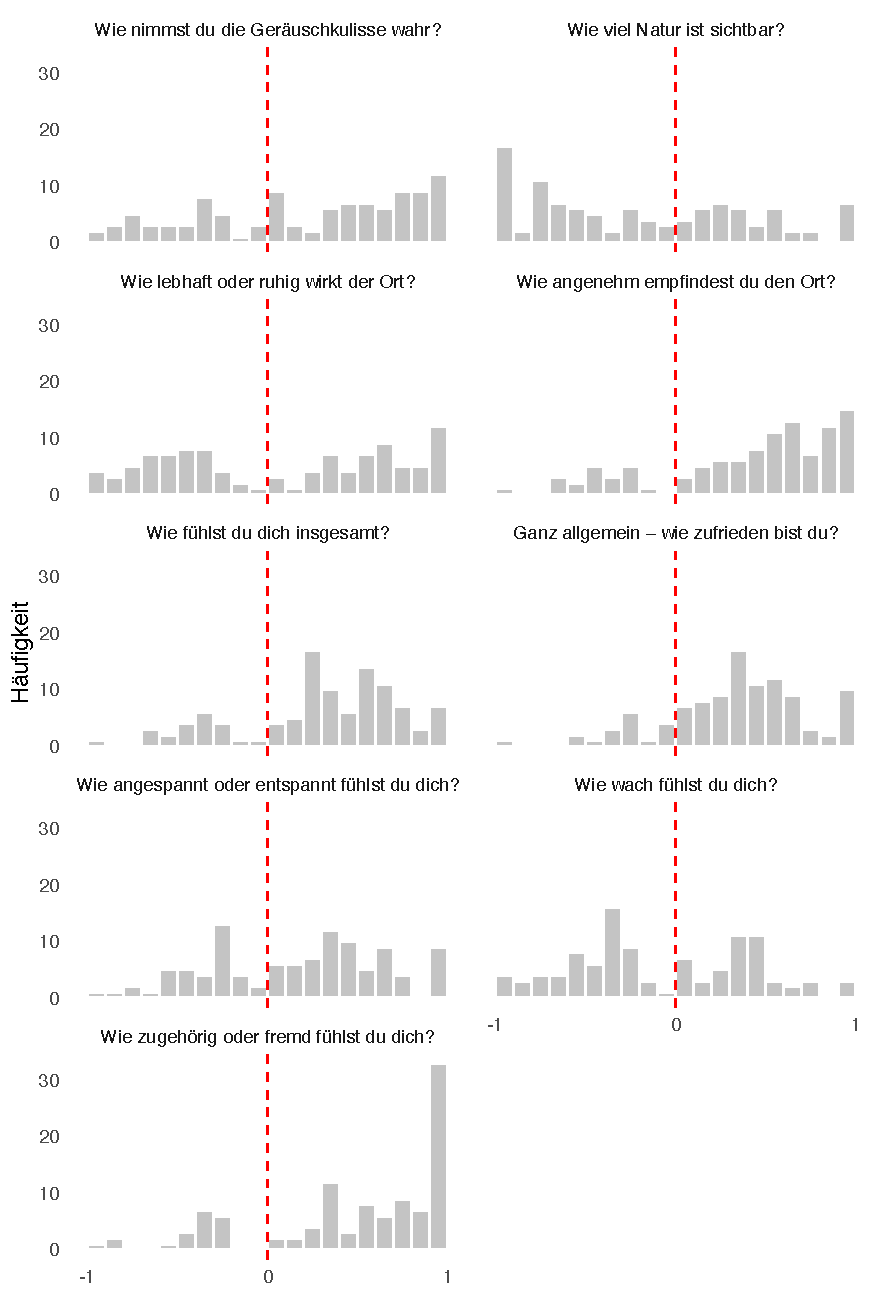
\includegraphics[width=\textwidth]{Analyse/Plots/slider_hists.pdf}
    \caption{Histogramme der Slider-Items}
    \label{fig:slider_hists}
\end{figure}

\begin{longtable}{p{5.5cm}p{9.5cm}}
    \caption{Antworten auf Freitextfragen}
    \label{tab:freitext}\\
    \toprule
    Frage & Antwort \\
    \midrule
    \endfirsthead

    \multicolumn{2}{c}{{\bfseries Tabelle \thetable{} -- Fortsetzung}} \\
    \toprule
    Frage & Antwort \\
    \midrule
    \endhead
    
    \midrule
    \multicolumn{2}{r}{Fortsetzung auf der nächsten Seite}\\
    \endfoot
    
    \bottomrule
    \endlastfoot

    Gibt es andere Dinge die dazu führen, dass Du dich hier weniger wohl oder unwohl fühlst? & heat \\*
     & Everyone is doing the same, so it kind of feels like being at the right place \\*
     & The contact with strangers \\*
     & Bed \\*
     & health issues \\*
     & no natural sunlight room without windows no fresh air \\*
     & a lot of people - personal space \\*
     & No \\*
     & / \\*
     & no \\*
     & Not really \\
    \midrule
    \addlinespace
    Gibt es andere Dinge die dazu führen, dass Du dich hier wohler fühlst? & place i know and is mine i have control over it \\*
     & know this place and can do what i want \\*
     & my room and cozy for the night \\*
     & pets \\*
     & spending time with family pets \\*
     & I am not by myself \\*
     & Less noise from construction works \\
    \bottomrule
\end{longtable}



\addtocontents{toc}{\protect\setcounter{tocdepth}{2}}

\end{appendices}
%TC:endignore
\end{document}